\documentclass{sybook}

\begin{document}
\begin{sloppypar}

% \title{学习笔记}
% \author{陈盛远}
% \date{\today}

\begin{titlepage}
    \centering

    %------------------------------------------------------------
    %    Top rules
    %------------------------------------------------------------

    \rule{\textwidth}{1pt}   % The top horizontal rule
    \vspace{0.2\textheight}  % Whitespace between top horizontal rule and title

    %------------------------------------------------------------
    %    Title
    %------------------------------------------------------------

    {\Huge 一本攻略}

    \vspace{0.025\textheight}   % Whitespace between the title and short horizontal rule

    \rule{0.83\textwidth}{0.4pt}  % The short horizontal rule under title

    \vspace{0.1\textheight}  % Whitespace between the short horizontal rule and author

    %------------------------------------------------------------
    %    Author
    %------------------------------------------------------------

    {\Large Author: \textsc{SY-Chen}}\\
    {\Large Email: sychenphy@163.com}

    \vfill  % Whitespace between author and date

    {\large \today}
    \vspace{0.1\textheight}  % Whitespace between date and bottom horizontal rule

    %------------------------------------------------------------
    %    Bottom rules
    %------------------------------------------------------------

    \rule{\textwidth}{1pt}  % The bottom horizontal rule
\end{titlepage}

\tableofcontents
\newpage
\setcounter{page}{1}

\part{预备数学知识}
\chapter{数学基础\label{chapter:reference}}

\section{微分}
\begin{note}
    函数$f(x_1, x_2, x_3\cdots)$包含多个变量时,其对自己的全导数为
    \begin{equation}
        \frac{d f}{d f} = \sum_{i} \frac{\partial f}{\partial x_i} \frac{\partial x_i}{\partial f}
    \end{equation}
\end{note}

%%%%%%%%%%%%%%%%%%%%%%%%%%%%%%%%%%%%%%%%%%%%%%%%%%%%%%%%%%%%%%%%%%%%%
\section{Cartesian坐标系与矢量\label{section:reference-cartesian}}
%%%%%%%%%%%%%%%%%%%%%%%%%%%%%%%%%%%%%%%%%%%%%%%%%%%%%%%%%%%%%%%%%%%%%

\subsection{坐标系}
Cartesian坐标系是直角坐标系和斜坐标系的统称。我们一般讨论的是直角坐标系,有二维的$xy$
坐标系和三维的$xyz$坐标系,这些坐标系下,每个轴都互相垂直。
\begin{figure}[h]
    \centering
    \setlength{\abovecaptionskip}{0.2cm}
    \inkfig{0.6}{./figure/math/CartesianCoord.pdf_tex}
    \caption{二维直角坐标系和三维直角坐标系}
    \label{fig:CartesianCoord}
\end{figure}

\subsection{矢量分析}
\begin{definition}[标量和矢量]
    标量指有大小无方向的量;矢量指有大小有方向的量。 
\end{definition}
常见的标量有温度、湿度、质量、电荷等;矢量有位移、速度、电场等。定义沿$x$、$y$和$z$轴
方向的单位矢量为$\vbe_x$、$\vbe_y$和$\vbe_z$。

\paragraph*{矢量操作}
\begin{enumerate}
    \item \textit{矢量加法}:矢量$\vec{\bm{b}}$的尾叠在矢量$\vec{\bm{a}}$的头上。一般表现为三角形
          规则或平行四边形规则。满足交换律和集合律
          \begin{align}
              \vec{\bm{a}} + \vec{\bm{b}} &= \vec{\bm{b}} + \vec{\bm{a}}
                                          \label{eq:vec-vec-add-exchang} \\
              \vec{\bm{a}} + (\vec{\bm{b}} + \vec{\bm{c}}) &= (\vec{\bm{a}} + \vec{\bm{b}}) + \vec{\bm{c}}
                                          \label{eq:vec-vec-add-combine}
          \end{align}
    \item \textit{标量与矢量乘法}:正值标量与矢量相乘只改变矢量大小不改变方向,负值标
          量与与矢量相乘改变矢量的大小和方向,$0$与矢量相乘永远标量为0。满足分配律
          \begin{equation}
              \begin{aligned}
                  a(\vec{\bm{a}} + \vec{\bm{b}}) &= a\vec{\bm{a}} + a\vec{\bm{b}} \\
                  (a + b) \vec{\bm{a}}     &= a\vec{\bm{a}} + b\vec{\bm{a}}
              \end{aligned}
            \label{eq:vec-distri}
          \end{equation}
    \item \textit{矢量与矢量点积}:两矢量点积定义为
           \begin{equation}
               \vec{\bm{a}} \cdot \vec{\bm{b}} = |\vec{\bm{a}}|\ |\vec{\bm{b}}|\cos{\theta}
            \label{eq:vec-dotproduct}
           \end{equation}
           $\theta$为$\vec{\bm{a}}$与$\vec{\bm{b}}$之间的夹角。满足交换律和分配律
           \begin{align}
               \vec{\bm{a}} \cdot \vec{\bm{b}} &= \vec{\bm{b}} \cdot \vec{\bm{a}}
                                           \label{eq:vec-vec-dot-exchange}   \\
               \vec{\bm{a}} \cdot (\vec{\bm{b}} + \vec{\bm{c}}) &= \vec{\bm{a}} \cdot \vec{\bm{b}} + \vec{\bm{a}} \cdot \vec{\bm{b}}
                                           \label{eq:vec-vec-dot-distri}
           \end{align}
    \item \textit{矢量与矢量叉积}:两矢量叉积定义为
          \begin{equation}
              \vec{\bm{a}} \times \vec{\bm{b}} = |\vec{\bm{a}}|\ |\vec{\bm{b}}|\sin{\theta} \hat{\vbn}
            \label{eq:vec-vec-cross}
          \end{equation}
          $\theta$为$\vec{\bm{a}}$与$\vec{\bm{b}}$之间的夹角,$\hat{\vbn}$为同时垂直与$\vec{\bm{a}}$和$\vec{\bm{b}}$的单
          位矢量。满足分配律
          \begin{equation}
              \vec{\bm{a}} \times(\vec{\bm{b}} + \vec{\bm{c}}) = \vec{\bm{a}} \times \vec{\bm{b}} + \vec{\bm{a}} \times \vec{\bm{c}}
                                            \label{eq:vec-vec-cross-distri}
          \end{equation}
          不满足交换律,但有
          \begin{equation}
              \vec{\bm{a}} \times \vec{\bm{b}} = - \vec{\bm{b}} \times \vec{\bm{a}}
            \label{eq:vec-vec-cross-exchange}
          \end{equation}
          $\vec{\bm{a}}$与$\vec{\bm{b}}$的叉积可理解为边长为$A$和$B$的平行四边形的面积,在乘上此
          四边形法向的单位向量。
      \item \textit{混合积1}:
            \begin{equation}
                \begin{aligned}
                    (\vec{\bm{a}} \times \vec{\bm{b}}) \cdot \vec{\bm{c}} 
                                        =& (\vec{\bm{b}} \times \vec{\bm{c}}) \cdot \vec{\bm{a}} \\
                                        =& (\vec{\bm{c}} \times \vec{\bm{a}}) \cdot \vec{\bm{b}} \\
                                        =&-(\vec{\bm{b}} \times \vec{\bm{a}}) \cdot \vec{\bm{c}} \\
                                        =&-(\vec{\bm{c}} \times \vec{\bm{b}}) \cdot \vec{\bm{a}} \\
                                        =&-(\vec{\bm{a}} \times \vec{\bm{c}}) \cdot \vec{\bm{b}} \\
                \end{aligned}
                \label{eq:vec-vec-vec-mix1}
            \end{equation}
            \CJKunderdot{注意}:上式第一个等号右边的乘积顺序是
            $\vec{\bm{a}} \rightarrow \vec{\bm{b}} \rightarrow \vec{\bm{c}}$,前两个等号右边式子从$\vec{\bm{a}}$开始也遵
            循同样的规律,因此其前面符号为正;最后三个等号从$\vec{A}$开始的顺序为
            $\vec{\bm{a}} \rightarrow \vec{\bm{c}} \rightarrow \vec{\bm{b}}$,顺序不再与第一个式子相同,
            出现负号。
      \item \textit{混合积2}:
          \begin{equation}
          \vec{\bm{a}} \times (\vec{\bm{b}} \times \vec{\bm{c}}) = \vec{\bm{b}}(\vec{\bm{a}} \cdot \vec{\bm{c}}) - \vec{\bm{c}}(\vec{\bm{a}} \cdot \vec{\bm{b}})
                                                        \label{eq:vec-vec-vec-mix2}
          \end{equation}
\end{enumerate}

三维直角坐标系沿坐标轴正方向定义三个正交的单位矢量$\vbe_x$、$\vbe_y$和$\vbe_z$,
他们之间的关系为
\begin{equation}
    \begin{aligned}
        \vbe_{i} \cdot  \vbe_{j} =& \delta_{ij} \\
        \vbe_{i} \times \vbe_{j} =& \epsilon_{ijk} \vbe_{k}
    \end{aligned}
    \label{eq:vec-cartesian}
\end{equation}
$\epsilon_{ijk}$为Levi-Civita符号,是一三阶反对称张量,满足
\begin{equation}
    \begin{aligned}
        \epsilon_{ijk} =& - \epsilon_{jik} = -\epsilon_{ikj} \\
        \epsilon_{123} =& 1
    \end{aligned}
    \label{eq:Levi-Civita}
\end{equation}
角坐标系中任一矢量都可由这三个单位矢量经线性组合构成,进而定义矢量与矢量、矢量与标
量间的运算规则。

%%%%%%%%%%%%%%%%%%%%%%%%%%%%%%%%%%%%%%%%%%%%%%%%%%%%%%%%%%%%%%%%%%%%%
\subsection{矢量运算}
\paragraph*{导数}
对于一个单变量函数$f(x)$,它的导数$\mathrm{d} f(x)/ \mathrm{d} x$表明它变化的快慢
\begin{equation}
    \mathrm{d} f = \frac{\mathrm{d} f}{\mathrm{d} x} dx
                                \label{eq:vec-derivative}
\end{equation}
上式可以表示为当$x$变化为$\mathrm{d}x$时,$f$变化为$\mathrm{d}f$,而导数则是这两个变
化值间的一个因子。几何上则将导数解释为$f$对$x$的斜率。

\paragraph*{$\nabla$算符}
定义$\nabla$算符为
\begin{equation}
    \nabla =    \vbe_x \frac{\partial}{\partial x} 
               +\vbe_y \frac{\partial}{\partial y}
               +\vbe_z \frac{\partial}{\partial z}
    \label{eq:def-nabla-cartesian}
\end{equation}
$\nabla$算符本身具有矢量的特性,但若不作用在函数上的话这个符号就没有任何意义。有三种
作用方式:
\begin{enumerate}
    \item 作用于一个标量函数$T$上:$\nabla T$(梯度)
    \item 通过点积作用到矢量函数$\vec{v}$上:$\nabla \cdot \vec{v}$(散度)
    \item 通过叉积作用到矢量函数$\vec{v}$上:$\nabla \times \vec{v}$(旋度)
\end{enumerate}

\paragraph*{梯度}
梯度是针对标量函数$T$,它的梯度是单变量导数的推广,写为
\begin{equation}
    \nabla T =   \frac{\partial T}{\partial x}\vbe_x 
               + \frac{\partial T}{\partial y}\vbe_y
               + \frac{\partial T}{\partial z}\vbe_z
    \label{eq:vec-gradient}
\end{equation}
\uline{梯度具有大小和方向}。梯度$\nabla T$所指方向是函数$T$具有最大增加的方向,
$|\nabla T|$代表这个最大增加方向的斜率。同样的,梯度为$0$标志着极大、极小或平直。

\CJKunderdot{有关梯度的基本定理}:对一个三变量的标量函数$T(x, y, z)$,从$a$点出发,
选定任意一条路径$P$,每次移动一个微小位移,直至最后到达点$b$,那么$T$沿着这个路径的
总改变量为
\begin{equation}
    \int_{a}^{b} (\nabla T) \cdot \mathrm{d} \vec{l}_{P} = T(b) - T(a)
    \label{eq:vec-gradiant-basictheorem}
\end{equation}
从式\eqref{eq:vec-gradiant-basictheorem}可看出,该路径积分只与路径始末端有关,而与路
径无关。从中可得到两个推论:
\begin{itemize}
    \item \textit{推论1}:梯度的路径积分只与路径边界值相关而与所选路径无关;
    \item \textit{推论2}:当所选路径闭合时,梯度对该路径的积分为零。
\end{itemize}

\paragraph*{散度}
散度是针对矢量函数的,一个标量函数的散度是无意义的。一个矢量函数$\vec{v}(x, y, z)$的
散度是一个标量
\begin{equation}
    \nabla \cdot \vbv = (   \vbe_x \frac{\partial T}{\partial x} 
                             + \vbe_y \frac{\partial T}{\partial y}
                             + \vbe_z \frac{\partial T}{\partial z})
                           \cdot
                           (\vbv_x + \vbv_y + \vbv_z)
    \label{eq:vec-devergence}
\end{equation}

\uline{几何解释}:散度是指矢量场在某一点出散出的量度,描述的是发散的程度,而发散是具
有方向的一个动作,因而散度是针对矢量而言的。具体如下图所示
\begin{figure}[ht]
    \centering
    \setlength{\abovecaptionskip}{0.2cm}
    \subfloat[]{
        \begin{tikzpicture}
    \draw[-Stealth, line width=1pt]             (0, 0) -- (0.8, 0);
    \draw[-Stealth, line width=1pt, rotate=30]  (0, 0) -- (0.8, 0);
    \draw[-Stealth, line width=1pt, rotate=60]  (0, 0) -- (0.8, 0);
    \draw[-Stealth, line width=1pt, rotate=90]  (0, 0) -- (0.8, 0);
    \draw[-Stealth, line width=1pt, rotate=120] (0, 0) -- (0.8, 0);
    \draw[-Stealth, line width=1pt, rotate=150] (0, 0) -- (0.8, 0);
    \draw[-Stealth, line width=1pt, rotate=180] (0, 0) -- (0.8, 0);
    \draw[-Stealth, line width=1pt, rotate=210] (0, 0) -- (0.8, 0);
    \draw[-Stealth, line width=1pt, rotate=240] (0, 0) -- (0.8, 0);
    \draw[-Stealth, line width=1pt, rotate=270] (0, 0) -- (0.8, 0);
    \draw[-Stealth, line width=1pt, rotate=300] (0, 0) -- (0.8, 0);
    \draw[-Stealth, line width=1pt, rotate=330] (0, 0) -- (0.8, 0);

    \draw[-Stealth, line width=1pt]             (1, 0) -- (2.5, 0);
    \draw[-Stealth, line width=1pt, rotate=30]  (1, 0) -- (2.5, 0);
    \draw[-Stealth, line width=1pt, rotate=60]  (1, 0) -- (2.5, 0);
    \draw[-Stealth, line width=1pt, rotate=90]  (1, 0) -- (2.5, 0);
    \draw[-Stealth, line width=1pt, rotate=120] (1, 0) -- (2.5, 0);
    \draw[-Stealth, line width=1pt, rotate=150] (1, 0) -- (2.5, 0);
    \draw[-Stealth, line width=1pt, rotate=180] (1, 0) -- (2.5, 0);
    \draw[-Stealth, line width=1pt, rotate=210] (1, 0) -- (2.5, 0);
    \draw[-Stealth, line width=1pt, rotate=240] (1, 0) -- (2.5, 0);
    \draw[-Stealth, line width=1pt, rotate=270] (1, 0) -- (2.5, 0);
    \draw[-Stealth, line width=1pt, rotate=300] (1, 0) -- (2.5, 0);
    \draw[-Stealth, line width=1pt, rotate=330] (1, 0) -- (2.5, 0);
\end{tikzpicture}

        \label{fig:vec-diverg-a}
    }
    \hfill
    \subfloat[]{
        \begin{tikzpicture}
    \draw[-Stealth, line width=1pt]               (0.0, 0.0) -- (0.0, 2.0);
    \draw[-Stealth, line width=1pt]               (0.0, 2.2) -- (0.0, 4.2);
    \draw[-Stealth, line width=1pt]               (0.6, 0.8) -- (0.6, 2.8);
    \draw[-Stealth, line width=1pt]               (0.6, 3.0) -- (0.6, 5.0);

    \draw[-Stealth, line width=1pt, xshift=1.2cm] (0.0, 0.0) -- (0.0, 2.0);
    \draw[-Stealth, line width=1pt, xshift=1.2cm] (0.0, 2.2) -- (0.0, 4.2);
    \draw[-Stealth, line width=1pt, xshift=1.2cm] (0.6, 0.8) -- (0.6, 2.8);
    \draw[-Stealth, line width=1pt, xshift=1.2cm] (0.6, 3.0) -- (0.6, 5.0);

    \draw[-Stealth, line width=1pt, xshift=2.4cm] (0.0, 0.0) -- (0.0, 2.0);
    \draw[-Stealth, line width=1pt, xshift=2.4cm] (0.0, 2.2) -- (0.0, 4.2);
    \draw[-Stealth, line width=1pt, xshift=2.4cm] (0.6, 0.8) -- (0.6, 2.8);
    \draw[-Stealth, line width=1pt, xshift=2.4cm] (0.6, 3.0) -- (0.6, 5.0);

    \draw[-Stealth, line width=1pt, xshift=3.6cm] (0.0, 0.0) -- (0.0, 2.0);
    \draw[-Stealth, line width=1pt, xshift=3.6cm] (0.0, 2.2) -- (0.0, 4.2);
    \draw[-Stealth, line width=1pt, xshift=3.6cm] (0.6, 0.8) -- (0.6, 2.8);
    \draw[-Stealth, line width=1pt, xshift=3.6cm] (0.6, 3.0) -- (0.6, 5.0);
\end{tikzpicture}

        \label{fig:vec-diverg-b}
    }
    \hfill
    \subfloat[]{
        \begin{tikzpicture}
    \draw[-Stealth, line width=1pt]               (0.0, 0.0) -- (0.0, 1.0);
    \draw[-Stealth, line width=1pt]               (0.0, 1.2) -- (0.0, 2.5);
    \draw[-Stealth, line width=1pt]               (0.0, 2.7) -- (0.0, 5.0);

    \draw[-Stealth, line width=1pt, xshift=0.6cm] (0.0, 0.0) -- (0.0, 1.0);
    \draw[-Stealth, line width=1pt, xshift=0.6cm] (0.0, 1.2) -- (0.0, 2.5);
    \draw[-Stealth, line width=1pt, xshift=0.6cm] (0.0, 2.7) -- (0.0, 5.0);

    \draw[-Stealth, line width=1pt, xshift=1.2cm] (0.0, 0.0) -- (0.0, 1.0);
    \draw[-Stealth, line width=1pt, xshift=1.2cm] (0.0, 1.2) -- (0.0, 2.5);
    \draw[-Stealth, line width=1pt, xshift=1.2cm] (0.0, 2.7) -- (0.0, 5.0);

    \draw[-Stealth, line width=1pt, xshift=1.8cm] (0.0, 0.0) -- (0.0, 1.0);
    \draw[-Stealth, line width=1pt, xshift=1.8cm] (0.0, 1.2) -- (0.0, 2.5);
    \draw[-Stealth, line width=1pt, xshift=1.8cm] (0.0, 2.7) -- (0.0, 5.0);

    \draw[-Stealth, line width=1pt, xshift=2.4cm] (0.0, 0.0) -- (0.0, 1.0);
    \draw[-Stealth, line width=1pt, xshift=2.4cm] (0.0, 1.2) -- (0.0, 2.5);
    \draw[-Stealth, line width=1pt, xshift=2.4cm] (0.0, 2.7) -- (0.0, 5.0);

    \draw[-Stealth, line width=1pt, xshift=3.0cm] (0.0, 0.0) -- (0.0, 1.0);
    \draw[-Stealth, line width=1pt, xshift=3.0cm] (0.0, 1.2) -- (0.0, 2.5);
    \draw[-Stealth, line width=1pt, xshift=3.0cm] (0.0, 2.7) -- (0.0, 5.0);

    \draw[-Stealth, line width=1pt, xshift=3.6cm] (0.0, 0.0) -- (0.0, 1.0);
    \draw[-Stealth, line width=1pt, xshift=3.6cm] (0.0, 1.2) -- (0.0, 2.5);
    \draw[-Stealth, line width=1pt, xshift=3.6cm] (0.0, 2.7) -- (0.0, 5.0);
\end{tikzpicture}

        \label{fig:vec-diverg-c}
    }
    \caption{}
    \label{fig:vec-diverg}
\end{figure}
\newline
图\ref{fig:vec-diverg-a}中,在给定点处只有穿出的矢量,因此具有较大的正值散度(箭头外
指为正,内指为负);图\ref{fig:vec-diverg-b}中,取定某一点,穿入该点和穿出该点的矢量
的度量是一样的,因此其的散度为0;图\ref{fig:vec-diverg-c}中,取定某一点,穿入该点的
矢量比穿出该点的矢量的度量要小,因此具有正的散度。

\CJKunderdot{有关散度的基本定理}:散度定理又称为高斯定理、格林定理,表示为
\begin{equation}
    \int_{V} (\nabla \cdot \vbv)\ \mathrm{d} \tau
                         = \oint_{S} \vbv \cdot \mathrm{d} \vec{\bm{a}}
    \label{eq:div-basetheo}
\end{equation}
它指出,一个矢量函数散度在区域的体积分可以转化该矢量函数在该区域边界上的面积分值。我
们可将$\vbv$当成一个不可压缩的流,$\vbv$的通量是单位时间内流出表面的总流量
(式\eqref{eq:div-basetheo}左边)。某点处$\vbv$的散度表示该点产生或吸收流的量度(散度为正表
示放出流,散度为负表示吸收流),对于空间中某一区域,其在单位时间内产生(或吸收)的流等于流经
其表面的通量。


\paragraph*{旋度}
旋度只针对矢量,标量的旋度没有任何意义,矢量的旋度仍为一个矢量。对矢量$\vec{v}(x, y, z)$
的旋度定义为
\begin{equation}
    \nabla \times \vbv = 
    \left|\begin{matrix}
        \vbe_x               &   \vbe_y               &   \vbe_z   \\
        \partial / \partial x   &   \partial / \partial y   &   \partial / \partial y  \\
        v_x                     &   v_y                     &   v_z 
    \end{matrix}\right|
    \label{eq:vec-curl}
\end{equation}

\uline{几何解释}:旋度表示在所选点处漩涡状态的量度,按右手规则确定旋度的方向。如图中
所示的旋度就不为零。旋度很常见,比如大海中的漩涡。
\begin{figure}[ht]
    \centering
    \setlength{\abovecaptionskip}{0.2cm}
    \includegraphics[scale=1.3]{./figure/math/vec-curl.pdf}
    \caption{}
    \label{fig:vec-curl}
\end{figure}

%%%%%%%%%%%%%%%%
\subsection{积规则}
针对$\nabla$算符,标量由两种方式构建:
\begin{center}
    $fg$ \\
    $\vec{\bm{a}}\vec{\bm{b}}$
\end{center}
矢量由两种方式构建:
\begin{center}
    $f\vec{\bm{a}}$ \\
    $\vec{\bm{a}} \times \vec{\bm{b}}$
\end{center}

%%%%%%%%%%%%%%%%%%%%%%%%%%%%%%%%%%%%%%%%%%%%%%%%%%%%%%%%%%%%%%%%%%%%
\section{极坐标系\label{section:reference-polar}}
%%%%%%%%%%%%%%%%%%%%%%%%%%%%%%%%%%%%%%%%%%%%%%%%%%%%%%%%%%%%%%%%%%%%%
点$P$的位置在二维直角坐标系中用相互垂直的两个轴线的具体值$P(x, y)$表示,在极坐标中则
用两个不相干的参数$P(r, \theta)$表示,如下图:
如图\ref{fig:PolarCoord}。
\begin{figure}[ht]
    \centering
    \setlength{\abovecaptionskip}{0.2cm}
    \begin{tikzpicture}
    \draw[-Stealth, line width=1pt](0, 0) -- (4, 0);
    \node at (3.8, -0.2) {$x$};
    \draw[-Stealth,color=gray](0, 0) -- (0, 4);
    \node[color=gray] at (-0.2, 3.8) {$y$};
    \draw (2, 0) coordinate(A) -- (0, 0) coordinate (B)
         -- (2, 2) coordinate (C)[-Stealth,line width=1pt]
         pic [draw, "$\theta$", angle eccentricity=1.5] {angle};
    \fill [color=red] (canvas cs:x=2cm,y=2cm) circle (2pt);
    \node at (2.2, 2) [right] {$P(r, \theta)$};
    \node at (0.8, 1) {$r$};
    \node at (0, 0)   [below left]{$O$};
\end{tikzpicture}

    \caption{极坐标系}
    \label{fig:PolarCoord}
\end{figure}
其中,$r$表示$P$点与原点$O$的距离,取为$r\in [0, +\infty)$;$\theta$表示$OP$这条射线
与直角坐标系中的$x$轴间的夹角,取逆时针方向为正方向,取为$\theta \in [0, 2\pi)$,

极坐标系到直角坐标系的变换关系如下:
\begin{equation}
    \begin{cases}
        x = r \cos \theta   \\
        y = r \sin \theta
    \end{cases}
    \label{eq:polar-cartesian}
\end{equation}
直角坐标系到极坐标系变换关系为
\begin{equation}
    \begin{cases}
             r &= \sqrt{x^2 + y^2}   \\
        \theta &= \arctan \frac{y}{x} \quad (x \neq 0)
    \end{cases}
    \label{eq:cartesian-polar}
\end{equation}

%%%%%%%%%%%%%%%%%%%%%%%%%%%%%%%%%%%%%%%%%%%%%%%%%%%%%%%%%%%%%%%%%%%%%
\section{球坐标系}
%%%%%%%%%%%%%%%%%%%%%%%%%%%%%%%%%%%%%%%%%%%%%%%%%%%%%%%%%%%%%%%%%%%%%

%%%%%%%%%%%%%%%%%%%%%%%%%%%%%%%%%%%%%%%%%%%%%%%%%%%%%%%%%%%%%%%%%%%%%
\subsection{球坐标图像}
\paragraph*{球坐标}
三维Cartesian坐标系中点$P(x, y, z)$在球坐标系下的表示为$P(r, \theta, \varphi)$,各分
量定义\footnote{不同书中各分量表示符号不同,需明确定义。}如下:
\begin{itemize}
    \item $r$:$P$点到坐标原点的距离,取$r \in [0, \infty]$;
    \item $\theta$:$z$轴正方向与射线$OP$的夹角,称\textbf{极角(polar angle)},取
                    $\theta in [0, \pi]$;
    \item $\phi$:$x$轴正方向与射线$OP$在$xOy$平面投影$OP^{\prime}$间的夹角,
                  称\textbf{方位角(azimuthal angle)},取$\phi \in [0, 2\pi)$。
\end{itemize}
球坐标系下的正交单位向量为$\hat{\bm{e}}_r$、$\hat{\bm{e}}_\theta$和$\hat{\bm{e}}_\phi$
方向沿径向、极角和方位角。\CJKunderdot{需要注意的是,这些单位矢量随着位置变化的}。
\begin{figure}[ht]
    \centering
    \begin{minipage}{0.42\textwidth}
        \centering
        \setlength{\abovecaptionskip}{0.2cm}
        \includegraphics{./figure/math/SphericalCoordinates.pdf}
        \caption{球坐标系}
        \label{fig:SphererCoord} 
    \end{minipage}
    \begin{minipage}{0.42\textwidth}
        \centering
        \setlength{\abovecaptionskip}{0.2cm}
        \includegraphics[scale = 0.125]{./figure/math/sphere-vol-ele.png}
        \caption{球坐标系体积元}
        \label{fig:Spherer-Volele} 
    \end{minipage}
\end{figure}

\paragraph*{体积元}
体积元近似为一立方体,然后求其边长
\begin{itemize}
    \item 矢量在$r$方向的偏移为$dr$
    \item 矢量在$\theta$方向的微小偏移:$r\cdot  d\theta$
    \item 矢量在$\phi$方向的微小偏移相当于矢量在$xOy$平面上的投影$r\sin{\theta}$的偏移:$r\sin\theta\cdot d\phi$
\end{itemize}
最后得到体积元公式为
\begin{equation}
    dV = r^2 \sin{\theta} d\,r\ d\,\theta d\,\phi
\end{equation}

\paragraph*{球坐标到Cartesian坐标的转换}
球坐标上某一点$\vec{\bm{P}}(r, \theta, \phi)$变换到Cartesian坐标的变换公式为
\begin{equation}
    \begin{aligned}
        \vbe_{x} 
       &= \vbe_{r}\sin\theta\cos\phi + \vbe_{\theta}\cos\theta\cos\phi - \vbe_{\phi}\sin{\phi} \\
        \vbe_{y} 
       &= \vbe_{r}\sin\theta\sin\phi + \vbe_{\theta}\cos\theta\sin\phi + \vbe_{\phi}\cos{\phi} \\
        \vbe_{z} 
       &= \vbe_{r}\cos\theta - \vbe_{\theta}\sin\theta
    \end{aligned}
    \label{eq:sphere-to-cartesian}
\end{equation}
写成矩阵形式为


%%%%%%%%%%%%%%%%%%%%%%%%%%%%%%%%%%%%%%%%%%%%%%%%%%%%%%%%%%%%%%%%%%%%%
\subsection{球坐标下的\texorpdfstring{$\nabla$}{}算符}
球坐标系下的$\nabla$算符可写为:
\begin{equation}
    \nabla =  \vbe_r \frac{\partial}{\partial r} 
            + \vbe_\theta \frac{\partial}{\partial \theta}
            + \vbe_\phi \frac{1}{r\sin{\theta}} \frac{\partial}{\partial \phi}
    \label{eq:nabla-sphere-form}
\end{equation}

球坐标系下标量场$T$和矢量场$\vbv$,矢量导数的坐标表示为,\newline
梯度:
\begin{equation}
    \nabla T = \frac{\partial T}{\partial r} \vec{\bm{e}}_r
              +\frac{1}{r} \frac{\partial T}{\partial \theta} \vbe_{\theta}
              +\frac{1}{r\sin{\theta}}\frac{\partial T}{\partial \phi} \vbe_{\phi}
    \label{eq:sphere-gradient}
\end{equation}
散度:
\begin{equation}
    \nabla \cdot \vbv = \frac{1}{r^2} \frac{\partial}{\partial r}(r^2 v_r)
      + \frac{1}{r\sin{\theta}}\frac{\partial}{\partial\theta}(\sin{\theta}\, v_{\theta})
      + \frac{1}{r\sin{\theta}}\frac{\partial}{\partial\phi} v_{\phi}
    \label{eq:sphere-divergence}
\end{equation}
旋度:
\begin{equation}
    \nabla \times \vec{\bm{v}} =
    \frac{1}{r\sin{\theta}}\left[ \frac{\partial}{\partial\theta}(\sin{\theta}\,v_{\phi}) 
                      - \frac{\partial v_{\theta}}{\partial\phi}\right] \vbe_r
     +\frac{1}{r} \left[ \frac{1}{\sin{\theta}} \frac{\partial v_{r}}{\partial \phi} 
                 - \frac{\partial}{\partial r}(r v_{\phi})\right] \vbe_{\theta}
     +\frac{1}{r}\left[\frac{\partial}{\partial r}(r v_{\theta})
                 - \frac{\partial v_{r}}{{\partial \theta}} \right] \vbe_{\phi}
    \label{eq:sphere-curl}
\end{equation}

%%%%%%%%%%%%%%%%%%%%%%%%%%%%%%%%%%%%%%%%%%%%%%%%%%%%%%%%%%%%%%%%%%%%%
\section{矢量与标量的分类}
%%%%%%%%%%%%%%%%%%%%%%%%%%%%%%%%%%%%%%%%%%%%%%%%%%%%%%%%%%%%%%%%%%%%%
三维Cartesian坐标系中,定义宇称变换矩阵
\begin{equation}
    \bm{P} = \begin{pmatrix}
        -1  &   0   &   0   \\
         0  &  -1   &   0   \\
         0  &   0   &  -1 
    \end{pmatrix}
    \label{eq:inverse-matrix}
\end{equation}
其表示对坐标取负:$x\rightarrow -x$、$y\rightarrow -y$和$z\rightarrow -z$。通过上述变换矩
阵,我们可以将矢量分为\textbf{极矢量(polar vectors)}、\textbf{赝矢量(pseudovectors)或轴矢
量(axial vectors)};标量分为\textbf{标量(scalar)}、\textbf{赝标量(pseudoscalar)}。

\paragraph*{极矢量}
对任意矢量$\vec{\bm{V}}$,若宇称变换矩阵$\bm{P}$作用后使其符号发生改变,将其定义为极矢量,如下:
\begin{equation}
    \bm{P} \vec{\bm{V}} = -\vec{\bm{V}}
    \label{eq:polar-vector}
\end{equation}
如位置矢量$\vbr$和速度矢量$\vbv$。

\paragraph*{赝矢量(轴矢量)}
赝矢量定义为两个极矢量的叉乘
\begin{equation}
    \vec{\bm{V}}^{\ast} = \vec{\bm{V}}_1 \times \vec{\bm{V}}_2
    \label{eq:pesudovectors-def}
\end{equation}
如角动量$\vbl = \vbr \times \vbp$就是赝矢量,其特征就是当宇称矩阵$\bm{P}$作用其上不改变它的
符号:
\begin{equation}
    \bm{P} \vec{\bm{V}}^{\ast} = (\bm{P} \vec{\bm{V}}_1) \times (\bm{P} \vec{\bm{V}}_1) = \vec{\bm{V}}^{\ast}
    \label{eq:pesudovec-parity}
\end{equation}
例如,角动量$\vbl = \vbr \times \vbp$是一个赝矢量,它由位置矢量$\vbr$和动量矢量$\vbp$这两
个矢量的叉乘得到,当宇称变换矩阵作用上去后,位置矢量和动量矢量符号都发生了改变,故最后得到
的角动量符号不发生变化。
\begin{note}
    若宇称算符作用在坐标轴上,虽然赝矢量的符号不变,但它相对坐标轴的方向确实是变化了的;若
    坐标轴发生变化,则整个坐标系统从右手系变到了左手系。
\end{note}

\paragraph*{标量}
标量$S$定义为
\begin{equation}
    \bm{P} S = S
    \label{eq:scalar-def}
\end{equation}
也就是说标量仅有大小而没有方向。

\paragraph*{赝标量}
赝标量$S^{\ast}$定义为
\begin{equation}
    S^{\ast} = \vec{\bm{V}} \cdot \vec{\bm{V}}^{\ast}
    \label{eq:pseudoscalar-def}
\end{equation}
如此,宇称变换算符$\bm{P}$作用后,赝标量符号改变
\begin{equation}
    \bm{P} S^{\ast} = \bm{P} (\vec{\bm{V}} \cdot \vec{\bm{V}}^{\ast}) = (\bm{P} \vec{\bm{V}}) \cdot (\bm{P}\vec{\bm{V}}^{\ast})
                  = -\vec{\bm{V}} \cdot \vec{\bm{V}}^{\ast} = -S^{\ast}
    \label{eq:pseudoscalar-prop1}
\end{equation}


%%%%%%%%%%%%%%%%%%%%%%%%%%%%%%%%%%%%%%%%%%%%%%%%%%%%%%%%%%%%%%%%%%%%%
\section{矢量场理论}
%%%%%%%%%%%%%%%%%%%%%%%%%%%%%%%%%%%%%%%%%%%%%%%%%%%%%%%%%%%%%%%%%%%%%
\paragraph{势函数}
若一个矢量场$\vec{\bm{f}}$的旋度处处为0,则$\vec{\bm{f}}$可表示为一个标量势$V$的梯度
\begin{equation}
    \nabla \times \vec{\bm{f}} = 0 \Leftrightarrow \vec{\bm{f}} = -\nabla V
    \label{eq:scalar-poten}
\end{equation}
\begin{proof}
    必要性,上面左边等式
    \begin{equation*}
        \vec{\bm{f}} = - \nabla V = -\vbe_x \frac{\partial V_x}{\partial x}
                            -\vbe_y \frac{\partial V_y}{\partial y}
                            -\vbe_z \frac{\partial V_z}{\partial z}
    \end{equation*}
    因此有
    \begin{equation*}
        \nabla \times \vec{\bm{F}} = \left|\begin{matrix}
            \vbe_x  &   \vbe_y  &   \vbe_z  \\
            \frac{\partial}{\partial x} & \frac{\partial}{\partial y} & \frac{\partial}{\partial z} \\
            -\frac{\partial V}{\partial x} & -\frac{\partial V}{\partial y} & -\frac{\partial V}{\partial z}
        \end{matrix}\right|
        = 0
    \end{equation*}
    充分性,待补充。
\end{proof}

\begin{theorem}[无旋场]
    以下条件等价:
    \begin{enumerate}
        \item 对任何一点满足$\nabla \times \vec{\bm{f}} = 0$;
    \end{enumerate}
\end{theorem}

%%%%%%%%%%%%%%%%%%%%%%%%%%%%%%%%%%%%%%%%%%%%%%%%%%%%%%%%%%%%%%%%%%%%%
\section{一些重要结论}
%%%%%%%%%%%%%%%%%%%%%%%%%%%%%%%%%%%%%%%%%%%%%%%%%%%%%%%%%%%%%%%%%%%%%
列出一些经常用到的公式计算结果及证明.

%%%%%%%%%%%%%
\section{行列式}

\subsection{余子式}
对$n$阶行列式$|\bm{A}|$,去掉其矩阵元$a_{ij}$所在行和列的所有元素后,留下的$n-1$阶行列式$|\bm{M}_{ij}|$为矩阵元$a_{ij}$对应的余子式。

\begin{example}
    $|\bm{A}|$是$3\times 3$的矩阵
    \begin{equation*}
    |\bm{A}| = \begin{vmatrix}
        a_{11} & a_{12} & a_{13} \\
        a_{21} & a_{22} & a_{23} \\
        a_{31} & a_{32} & a_{33}
    \end{vmatrix}
    \end{equation*}
    其矩阵元$a_{11}$对应的余子式为
    \begin{equation*}
    |\bm{M}_{ij}| = \begin{vmatrix}
        a_{22} & a_{23} \\
        a_{32} & a_{33}
    \end{vmatrix}
    \end{equation*}
\end{example}

%%%%%%%%%%%
\subsection{代数余子式}
矩阵元$a_{ij}$对应的代数余子式表示为
\begin{equation}
    |\bm{A}_{ij}| = (-)^{i+j} |\bm{M}_{ij}|
\end{equation}

\section{矩阵}

定义$\bm{I}$为单位矩阵
\begin{equation}
    \bm{I} = \begin{pmatrix}
        1 &   &          \\
          & 1 &          \\
          &   &  \ddots  \\
    \end{pmatrix}
\end{equation}

\paragraph*{矩阵的一些约定}
\begin{enumerate}
    \item 矩阵用粗体大写字母或圆括号包裹其中元素(对应的小写字母,下表表示对应的行和列)表示
        \begin{equation}
            \bm{A} = (a_{ij})
        \end{equation}
    \item 转置矩阵 $\bm{A}^{T}$ 或 $(a^{T}_{ij})$
    \item 逆矩阵 $\bm{A}^{-1}$ 或 $(a^{-1}_{ij})$。
    \item 伴随矩阵 $\bm{A}^{adj}$。
\end{enumerate}

%%%%%%%%%%%%
\subsection{伴随矩阵}
矩阵$\bm{A}$的伴随矩阵用其代数余子式表示为
\begin{equation}
    \bm{A}^{adj} = \begin{pmatrix}
        |\bm{A}_{11}| & |\bm{A}_{21}| & \cdots & |\bm{A}_{n1}| \\
        |\bm{A}_{12}| & |\bm{A}_{22}| & \cdots & |\bm{A}_{n2}| \\
        \vdots        & \vdots        & \ddots & \vdots        \\
        |\bm{A}_{1n}| & |\bm{A}_{2n}| & \cdots & |\bm{A}_{nn}|
    \end{pmatrix}
    \label{eq:adjoint-mat}
\end{equation}
其跟矩阵$\bm{A}$的关系为
\begin{equation}
    \bm{A}\bm{A}^{adj} = |\bm{A}|\bm{I}
    \label{eq:corr-mat-adjmat}
\end{equation}

%%%%%%%%%%%%
\subsection{逆矩阵}
矩阵$\bm{A}$的逆矩阵$\bm{A}^{-1}$满足
\begin{equation}
    \bm{A}\bm{A}^{-1} = \bm{A}^{-1}\bm{A} = \bm{I}
    \label{eq:inverse-mat}
\end{equation}
根据\cref{eq:corr-mat-adjmat,eq:inverse-mat},伴随矩阵与逆矩阵矩阵元$a^{-1}_{ij}$间的关系为
\begin{equation}\boxed{
        a^{-1}_{ij} = \frac{\bm{A}^{adj}_{ji}}{|\bm{A}|}
    \label{eq:corr-adjmat-invmat}
}\end{equation}

\section{本征值与本征矢}

\begin{definition}[本征值与本征矢]
  $\bm{A}$是$n$阶方阵,若存在数$\lambda$和非零矢量$\bm{x}$,使得$\bm{Ax}=\lambda \bm{x}$ ($\bm{x}\neq \bm{0}$),则$\lambda$为方阵$\bm{A}$的本征值,$\bm{x}$为对应的本征矢。
\end{definition}

\section{矩阵的迹}
矩阵的迹为其对角元之和,矩阵的迹又如下性质:
\begin{enumerate}
\item Linear property:
\begin{equation}
    {\rm Tr}(A+B) = {\rm Tr}(A) +{\rm Tr}(B)  \label{tracelinear}
\end{equation}

\item Multiplicity property:
\begin{equation}
    {\rm Tr}(cA) = c{\rm Tr}(A)  \label{tracemulti}
\end{equation}

\item Cyclic property:
\begin{equation}
  \begin{aligned}
    {\rm Tr}(AB) =& {\rm Tr}(BA)\\  \label{tracecyclic}
    {\rm Tr}[A,B]C =& {\rm Tr}A[B,C]
  \end{aligned}
\end{equation}
\end{enumerate}


\section{The Jacobi identity}
\begin{theorem}{The Jacobi identity}{}
  For three matrices $A, B$ and $C$, we have the identical relation
  \begin{equation}
    \left[A, [B,C]\right] + \left[C, [A,B]\right] + \left[B, [C,A]\right] = 0 \label{Jacobidentity}
  \end{equation}
\end{theorem}

%%%%%%%%%%%%%%%%%%%%%%
\section{行列式的导数}

\subsection{行列式对矩阵元的导数}
方阵$\bm{A}$对应的行列式为$|\bm{A}|$,它可以写成代数余子式$\bm{C_{ij}}$的求和
\begin{equation}
    |\bm{A}| = \sum_{j} a_{ij} |\bm{A}_{ij}|
    \label{eq:rep-cofactor}
\end{equation}
这样,该行列式对其中某一元素的导数为
\begin{equation}\boxed{
    \frac{\partial |\bm{A}|}{\partial a_{ij}} = \sum_{j} \frac{\partial \left(a_{ij} |\bm{A}_{ij}|\right)}{\partial a_{ij}} = |\bm{A}_{ij}|
    \label{eq:Det-part-elem}
}\end{equation}
上述表明行列式对某一元素的导数为其元素对应的代数余子式。

\subsection{行列式对其他变量的导数}
行列式中所有元素都是变量$t$的函数:$a_{ij}(t)$。由\cref{eq:Det-part-elem},根据变量$t$的求导用连续偏导方程展开
\begin{equation*}
    \frac{d |\bm{A}|}{d t} = \sum_{ij} \frac{\partial |\bm{A}|}{\partial a_{ij}} \frac{\partial a_{ij}}{\partial t} = \sum_{ij} |\bm{A}_{ij}| \frac{\partial a_{ij}}{\partial t} = |\bm{A}| \sum_{ij} \frac{|\bm{A}_{ij}|}{|\bm{A}|} \frac{d a_{ij}}{d t}
\end{equation*}
$\cfrac{d a_{ij}}{d t}$是$\cfrac{d \bm{A}}{d t}$的矩阵元,根据\cref{eq:corr-adjmat-invmat},上式最后一个等号改写为
\begin{equation*}
    |\bm{A}| \sum_{ji} (a)^{-1}_{ji} \left(\frac{d \bm{A}}{d t}\right)_{ij}
    =
    |\bm{A}| \sum_{j} \left( \bm{A}^{-1} \frac{d \bm{A}}{d t} \right)_{jj}
    = 
    |\bm{A}| {\rm Tr} \left( \bm{A}^{-1} \frac{d \bm{A}}{d t} \right)
\end{equation*}
所以最后有
\begin{equation}\boxed{
    \frac{d |\bm{A}|}{d t} = 
    |\bm{A}| {\rm Tr} \left( \bm{A}^{-1} \frac{d \bm{A}}{d t} \right)
    \label{eq:mat-der-var}
}\end{equation}

由\cref{eq:mat-der-var}可知,包含对数的求导$\cfrac{d \ln{|\bm{A}|}}{d t}$的求导过程为
\begin{equation}\boxed{
    \frac{\ln{|\bm{A}|}}{d t} = \frac{1}{|\bm{A}|} \frac{d |\bm{A}|}{d t} = {\rm Tr} \left( \bm{A}^{-1} \frac{d \bm{A}}{d t} \right)
    \label{eq:det-log-dev}
}\end{equation}

%%%%%%%%%%%%%%
\section{坐标变换}

\subsection{矩阵描述的坐标变换}
二维Cartesian坐标变换如\cref{fig:2dimCartesianCoordTrans}所示,表示$xOy$坐标系(基矢为$\vec{\bm{e}}_{x}$和$\vec{\bm{e}}_{y}$)绕坐标原点逆时针旋转$\theta$角后变为$x^{\prime}O^{\prime}y^{\prime}$坐标系(基矢为$\vec{\bm{e}}_{x}^{\prime}$和$\vec{\bm{e}}_{y}{\prime}$)。
\begin{figure}[htb]
    \centering
    \setlength{\abovecaptionskip}{0.2cm}
    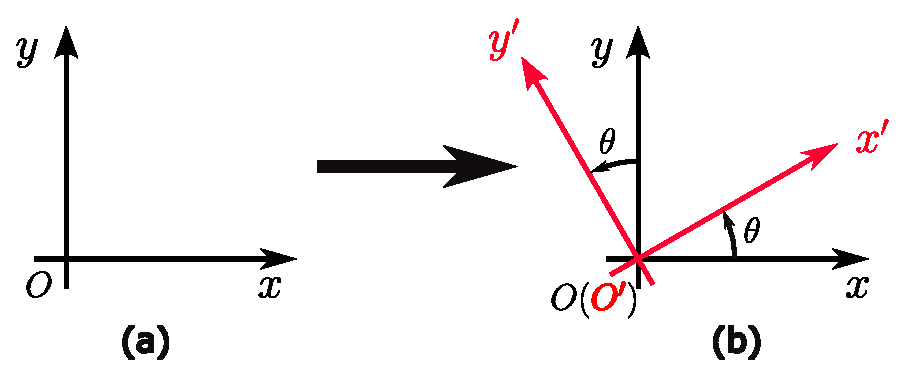
\includegraphics[scale=0.8]{figure/math/2dim-transform.eps}
    \caption{二维Cartesian坐标变换。}
    \label{fig:2dimCartesianCoordTrans}
\end{figure}

上述坐标变为相当于对基矢进行变化,从$xOy\Rightarrow x^{\prime}O^{\prime}y^{\prime}$的变换方程为
\begin{equation}\begin{aligned}
    \vec{\bm{e}}_{x}^{\,\prime} =& \vec{\bm{e}}_{x}\cos{\theta} + \vec{\bm{e}}_{y}\sin{\theta} \\
    \vec{\bm{e}}_{y}^{\,\prime} =& -\vec{\bm{e}}_{x}\sin{\theta} + \vec{\bm{e}}_{y}\cos{\theta}
    \label{eq:rot-char-eq}
\end{aligned}\end{equation}
其对应的逆变换($x^{\prime}O^{\prime}y^{\prime} \Rightarrow xOy$)为
\begin{equation}\begin{aligned}
    \vec{\bm{e}}_{x} =& \vec{\bm{e}}_{x}^{\,\prime}\cos{\theta} - \vec{\bm{e}}_{y}^{\,\prime}\sin{\theta} \\
    \vec{\bm{e}}_{y} =& \vec{\bm{e}}_{x}^{\,\prime}\sin{\theta} + \vec{\bm{e}}_{y}^{\,\prime}\cos{\theta}
    \label{eq:inver-rot-char-eq}
\end{aligned}\end{equation}

此变换可用矩阵来表示,假定矩阵$\bm{R}(\theta)$的作用是将矢量绕原点逆时针旋转$\theta$角(表示方程\cref{eq:rot-char-eq}),则$\bm{R}^{-1}(\theta) = \bm{R}(-\theta)$表示将矢量绕坐标原点顺时针旋转$\theta$角(表示\cref{eq:inver-rot-char-eq}),则\cref{fig:2dimCartesianCoordTrans}中坐标系的变换可写为
\begin{equation}
    \bm{R}(\theta) = \begin{pmatrix}
        \cos{\theta} & \sin{\theta} \\
        -\sin{\theta} & \cos{\theta}
    \end{pmatrix},
    \qquad
    \bm{R}^{-1}(\theta) = \bm{R}(-\theta) = \begin{pmatrix}
        \cos{\theta} & -\sin{\theta} \\
        \sin{\theta} & \cos{\theta}
    \end{pmatrix}
\end{equation}
因此\cref{eq:rot-char-eq,eq:inver-rot-char-eq}又可用矩阵表述为如下形式
\begin{equation*}
    \begin{pmatrix}
        \vec{\bm{e}}_{x} \\
        \vec{\bm{e}}_{y}
    \end{pmatrix}
    = \bm{R} \begin{pmatrix}
        \vec{\bm{e}}_{x}^{\,\prime} \\
        \vec{\bm{e}}_{y}^{\,\prime}
    \end{pmatrix},
    \qquad
    \begin{pmatrix}
        \vec{\bm{e}}_{x}^{\,\prime} \\
        \vec{\bm{e}}_{y}^{\,\prime}
    \end{pmatrix}
    = \bm{R}^{-1} \begin{pmatrix}
        \vec{\bm{e}}_{x} \\
        \vec{\bm{e}}_{y}
    \end{pmatrix}
\end{equation*}

\subsection{用复数表示的转动}
用复数可以表示绕定点或定轴的转动。具体可参考\href{https://www.cnblogs.com/noluye/p/11964513.html}{网页链接}。二维空间中可认为是绕$z$轴或原点的转动,三维空间中可描述在垂直于定轴的平面上的转动。

此时,转动算符$\bm{R}(\theta)$与${\rm e}^{i\theta}$的作用是一致的。

\section{张量}

\include{contents/math-base/interpolation-method}
\chapter{数值积分}

\section{一维数值积分}
\subsection{辛普森积分及复合辛普森积分}
\paragraph*{辛普森积分} 区间$[a, b]$有函数$f(x)$,求函数在此区间内的积分,可定义此区间的中点$\dfrac{a+b}{2}$及对应的函数值$f(\dfrac{a+b}{2})$,也就是对区间$[a, b]$进行二等分,这样,对应的数值积分为
\begin{equation}
	I = \int_{a}^{b} f(x) \, dx \approx \frac{h}{6}\left[ f(a) + f(\frac{a+b}{2}) + f(b) \right]	\label{eq:simpson-integer}
\end{equation} 

\paragraph*{复合辛普森积分} 区间$[a, b]$内有函数$f(x)$,现将区间$n$等分,在区间$[x_{k}, x_{k+1}](k = 0, 1, 2, \cdots, n-1)$内应用式\eqref{eq:simpson-integer},并对每个小区间进行累加,这样就可以得到整个区间内的积分。设$x_{k+1/2} = \dfrac{x_k + x_{k+1}}{2}$,这样,$[a, b]$区间内对$f(x)$的积分为
\begin{equation}
    \begin{aligned}
		I =& \int_{a}^{b} f(x) \, dx = \sum_{i = 0}^{n - 1}\int_{x_i}^{x_{i+1}} f(x) \, dx	\\
		=& \frac{h}{6}\sum_{i=1}^{n-1} \left[ f(x_i) + 4f(x_{k+1/2}) + f(x_{k+1})  \right] + R_n(f)
    \end{aligned}
\end{equation} 
取近似
\begin{equation}
    \begin{aligned}
    	I \approx S_n = \frac{h}{6}\sum_{i=1}^{n-1} \left[ f(x_i) + 4f(x_{k+1/2}) + f(x_{k+1})  \right]
    \end{aligned}
\end{equation} 
上式称为\uline{复合辛普森积分}。余项为
\begin{equation}
	R_n(f) = I - S_n = -\frac{h}{180} \left(\frac{h}{2} \right) \sum_{i = 0}^{n-1}f^{(4)}(\eta_i), \quad \eta_i \in (x_i, x_{i+1})
\end{equation} 
其中,$h = x_{i+1} - x_{k}$,误差阶为$h^4$。

\begin{example}
	\textbf{c++实现复合辛普森积分:} 考虑一些数据点,
	
\end{example}

\subsection{Cubic积分}
在完成cubic插值后,我们可根据方程\eqref{eq:unkown_Sx}求出原函数的近似,区间$[x_i, x_{i+1}]$区间内有函数$f(x)$,此时,我们有
\begin{equation}
	\begin{aligned}
		I_i =& \int_{x_i}^{x_{i+1}} f(x) \, dx \approx \int_{x_i}^{x_{i+1}} S(x) \, dx \\
		=& \int_{x_i}^{x_{i+1}} \, dx \left[ M_i \frac{\left(x_{i+1}-x\right)^3}{6 h_i}+M_{i+1} \frac{\left(x-x_i\right)^3}{6 h_i}+\left(y_i-\frac{M_i h_i^2}{6}\right) \frac{x_{i+1}-x}{h_i} \right. \\
		 &\left. + \left(y_{i+1}-\frac{M_{i+1} h_i^2}{6}\right) \frac{x-x_i}{h_i} \right]	\\
		=& \left[ -\frac{M_i}{24h_i} \left(x_{i+1}-x\right)^4 + \frac{M_{i+1}}{24h_i}\left(x-x_i\right)^4 \right. \\
		 &\left. -\left(y_i-\frac{M_i h_i^2}{6}\right) \frac{(x_{i+1}-x)^2}{2h_i} + \left(y_{i+1}-\frac{M_{i+1} h_i^2}{6}\right) \frac{(x-x_i)^2}{2h_i} + \text{Const} \right]_{x_i}^{x_{i+1}}	\\
		=& \frac{y_i + y_{i+1}}{2} h_i - \frac{M_{i} + M_{i+1}}{24} h_i^3
	\end{aligned}
\end{equation} 
其中,$h_i = x_{i+1}-x_{i}$。区间$[a,\ b]$存在函数$f(x)$,将此区间进行$n$等分,每个小区间
为$a = x_0 < x_1 < x_2 < \cdots < x_{n-1} < x_n = b $,求函数在此区域内的积分,如下
\begin{equation}
	I = \sum_{i=0}^{n-1} I_{i} \approx \sum_{i=0}^{n-1} \frac{y_i + y_{i+1}}{2} h_i - \frac{M_{i} + M_{i+1}}{24} h_i^3
\end{equation} 
当为等距格点时,即$h = h_0 = h_1 =\cdots = h_{n-1}$时,上式化为
\begin{equation}
	I\approx\frac{y_0+y_n+2\sum_{i=1}^{n-1}y_i}{2}h-\frac{M_0+M_n+2\sum_{i=1}^{n-1}M_i}{24}h^3
    \label{eq:cubic-int-equidistant}
\end{equation} 

Cubic一维积分程序见附录\ref{chap:code}。

\section{二维平面积分}
对二维笛卡尔坐标系$x-y$平面的积分,可先对$x$坐标积分,在对$y$坐标积分,这样可得到原函数在
二维平面上的积分。
\subsection{Cubic二维平面积分}
对于等间距的点,我们直接用式\eqref{eq:cubic-int-equidistant}来分别对$x$方向和$y$方向进行
积分。






%%%%%%%%%%%%%%%%%%%%%%%%%%%%%%%%%%%%%%%%%%%%%%%%%%%%%%%%%%%%%
% \chapter{数值微分}
% \section{五点数值微分公式}
% \subsection{二阶导微分公式}
% 设$f(x)$为定义在区间$[a,b]$上的函数,给定$f(x)$在等距点$a \leqslant x_0 < x_1 < x_2 < x_3
% < x_4 \leqslant b$,节点上函数值为$f(x_k)$,$(k=0, 1, 2, 3, 4)$,且满足$x_{k+1}-x_k=h$。
% 在$[a,b]$上做$f(x)$的4次Lagrange插值函数,并将$x=x_0+th, t \in [0, 4], x_k = x_0+kh$带入,
% 将方程两端对$t$求二次导,再分别把$t=0, 1, 2, 3, 4$带入,可得到$x_k$节点二阶导数的5点数值
% 微分公式,如下:
% \begin{equation}
% 	\begin{aligned}
% 		f^{\prime\prime}(x_0) =& \frac{1}{12h^2}[35f(x_0) - 104f(x_1) + 114f(x_2) - 56f(x_3) + 11f(x_4)] \\
% 		f^{\prime\prime}(x_1) =& \frac{1}{12h^2}[11f(x_0) -  20f(x_1) +   6f(x_2) +  4f(x_3) -   f(x_4)] \\
% 		f^{\prime\prime}(x_2) =& \frac{1}{12h^2}[ -f(x_0) +  16f(x_1) -  30f(x_2) + 16f(x_3) -   f(x_4)] \\
% 		f^{\prime\prime}(x_3) =& \frac{1}{12h^2}[ -f(x_0) +   4f(x_1) +   6f(x_2) - 20f(x_3) + 11f(x_4)] \\
% 		f^{\prime\prime}(x_4) =& \frac{1}{12h^2}[11f(x_0) -  56f(x_1) + 114f(x_2) -104f(x_3) + 35f(x_4)]
% 	\end{aligned}
% \end{equation} 





%%%%%%%%%%%%%%%%%%%%%%%%%%%%%%%%%%%%%%%%%%%%%%%%%%%%%%%%%%%%%
\chapter{数值微分}
\section{五点数值微分公式}
\subsection{二阶导微分公式}
设$f(x)$为定义在区间$[a,b]$上的函数,给定$f(x)$在等距点$a \leqslant x_0 < x_1 < x_2 < x_3
< x_4 \leqslant b$,节点上函数值为$f(x_k)$,$(k=0, 1, 2, 3, 4)$,且满足$x_{k+1}-x_k=h$。
在$[a,b]$上做$f(x)$的4次Lagrange插值函数,并将$x=x_0+th, t \in [0, 4], x_k = x_0+kh$带入,
将方程两端对$t$求二次导,再分别把$t=0, 1, 2, 3, 4$带入,可得到$x_k$节点二阶导数的5点数值
微分公式,如下:
\begin{equation}
	\begin{aligned}
		f^{\prime\prime}(x_0) =& \frac{1}{12h^2}[35f(x_0) - 104f(x_1) + 114f(x_2) - 56f(x_3) + 11f(x_4)] \\
		f^{\prime\prime}(x_1) =& \frac{1}{12h^2}[11f(x_0) -  20f(x_1) +   6f(x_2) +  4f(x_3) -   f(x_4)] \\
		f^{\prime\prime}(x_2) =& \frac{1}{12h^2}[ -f(x_0) +  16f(x_1) -  30f(x_2) + 16f(x_3) -   f(x_4)] \\
		f^{\prime\prime}(x_3) =& \frac{1}{12h^2}[ -f(x_0) +   4f(x_1) +   6f(x_2) - 20f(x_3) + 11f(x_4)] \\
		f^{\prime\prime}(x_4) =& \frac{1}{12h^2}[11f(x_0) -  56f(x_1) + 114f(x_2) -104f(x_3) + 35f(x_4)]
	\end{aligned}
\end{equation} 





%%%%%%%%%%%%%%%%%%%%%%%%%%%%%%%%%%%%%%%%%%%%%%%%%%%%%%%%%%%%%
\chapter{数学物理}

\section{球谐函数}
\subsection{球谐函数的定义}
球谐函数定义为
\begin{equation}
    Y_{l, m}(\theta, \phi) = (-1)^{m} \sqrt{\frac{(2l + 1)(l - m)!}{4\pi(l+m)!}} P_{l}^{m}(\cos{\theta}) e^{{\rm i}m\phi}
\end{equation}

\subsection{球谐函数的基本公式}
\paragraph*{复共轭}
\begin{equation}
    Y_{lm}^{\ast}(\theta, \phi) = (-1)^{m} Y_{l-m}(\theta, \phi)
    \label{eq:sp-ho}
\end{equation}

\paragraph*{三个球谐函数的积分}
\begin{equation}
    \begin{aligned}
        \int_{0}^{\pi}\sin{\theta}\, d\theta \int_{0}^{2\pi} d\phi
           Y_{l_1m_1} Y_{l_2m_2}Y_{l_3m_3}
        =& 
        \sqrt{\frac{(2l_1 + 1)(2l_2 + 1)(2l_3 + 1)}{4\pi}}
        \begin{pmatrix}
            l_1 & l_2 & l_3 \\
            0   & 0   & 0
        \end{pmatrix}
        \begin{pmatrix}
            l_1 & l_2 & l_3 \\
            m_1 & m_2 & m_3
        \end{pmatrix} \\
    \end{aligned}
\end{equation}
% \chapter{线性代数}

\section{行列式}

\subsection{余子式}
对$n$阶行列式$|\bm{A}|$,去掉其矩阵元$a_{ij}$所在行和列的所有元素后,留下的$n-1$阶行列式$|\bm{M}_{ij}|$为矩阵元$a_{ij}$对应的余子式。

\begin{example}
    $|\bm{A}|$是$3\times 3$的矩阵
    \begin{equation*}
    |\bm{A}| = \begin{vmatrix}
        a_{11} & a_{12} & a_{13} \\
        a_{21} & a_{22} & a_{23} \\
        a_{31} & a_{32} & a_{33}
    \end{vmatrix}
    \end{equation*}
    其矩阵元$a_{11}$对应的余子式为
    \begin{equation*}
    |\bm{M}_{ij}| = \begin{vmatrix}
        a_{22} & a_{23} \\
        a_{32} & a_{33}
    \end{vmatrix}
    \end{equation*}
\end{example}

%%%%%%%%%%%
\subsection{代数余子式}
矩阵元$a_{ij}$对应的代数余子式表示为
\begin{equation}
    |\bm{A}_{ij}| = (-)^{i+j} |\bm{M}_{ij}|
\end{equation}

\section{矩阵}

定义$\bm{I}$为单位矩阵
\begin{equation}
    \bm{I} = \begin{pmatrix}
        1 &   &          \\
          & 1 &          \\
          &   &  \ddots  \\
    \end{pmatrix}
\end{equation}

\paragraph*{矩阵的一些约定}
\begin{enumerate}
    \item 矩阵用粗体大写字母或圆括号包裹其中元素(对应的小写字母,下表表示对应的行和列)表示
        \begin{equation}
            \bm{A} = (a_{ij})
        \end{equation}
    \item 转置矩阵 $\bm{A}^{T}$ 或 $(a^{T}_{ij})$
    \item 逆矩阵 $\bm{A}^{-1}$ 或 $(a^{-1}_{ij})$。
    \item 伴随矩阵 $\bm{A}^{adj}$。
\end{enumerate}

%%%%%%%%%%%%
\subsection{伴随矩阵}
矩阵$\bm{A}$的伴随矩阵用其代数余子式表示为
\begin{equation}
    \bm{A}^{adj} = \begin{pmatrix}
        |\bm{A}_{11}| & |\bm{A}_{21}| & \cdots & |\bm{A}_{n1}| \\
        |\bm{A}_{12}| & |\bm{A}_{22}| & \cdots & |\bm{A}_{n2}| \\
        \vdots        & \vdots        & \ddots & \vdots        \\
        |\bm{A}_{1n}| & |\bm{A}_{2n}| & \cdots & |\bm{A}_{nn}|
    \end{pmatrix}
    \label{eq:adjoint-mat}
\end{equation}
其跟矩阵$\bm{A}$的关系为
\begin{equation}
    \bm{A}\bm{A}^{adj} = |\bm{A}|\bm{I}
    \label{eq:corr-mat-adjmat}
\end{equation}

%%%%%%%%%%%%
\subsection{逆矩阵}
矩阵$\bm{A}$的逆矩阵$\bm{A}^{-1}$满足
\begin{equation}
    \bm{A}\bm{A}^{-1} = \bm{A}^{-1}\bm{A} = \bm{I}
    \label{eq:inverse-mat}
\end{equation}
根据\cref{eq:corr-mat-adjmat,eq:inverse-mat},伴随矩阵与逆矩阵矩阵元$a^{-1}_{ij}$间的关系为
\begin{equation}\boxed{
        a^{-1}_{ij} = \frac{\bm{A}^{adj}_{ji}}{|\bm{A}|}
    \label{eq:corr-adjmat-invmat}
}\end{equation}

\section{本征值与本征矢}

\begin{definition}[本征值与本征矢]
  $\bm{A}$是$n$阶方阵,若存在数$\lambda$和非零矢量$\bm{x}$,使得$\bm{Ax}=\lambda \bm{x}$ ($\bm{x}\neq \bm{0}$),则$\lambda$为方阵$\bm{A}$的本征值,$\bm{x}$为对应的本征矢。
\end{definition}

\section{矩阵的迹}
矩阵的迹为其对角元之和,矩阵的迹又如下性质:
\begin{enumerate}
\item Linear property:
\begin{equation}
    {\rm Tr}(A+B) = {\rm Tr}(A) +{\rm Tr}(B)  \label{tracelinear}
\end{equation}

\item Multiplicity property:
\begin{equation}
    {\rm Tr}(cA) = c{\rm Tr}(A)  \label{tracemulti}
\end{equation}

\item Cyclic property:
\begin{equation}
  \begin{aligned}
    {\rm Tr}(AB) =& {\rm Tr}(BA)\\  \label{tracecyclic}
    {\rm Tr}[A,B]C =& {\rm Tr}A[B,C]
  \end{aligned}
\end{equation}
\end{enumerate}


\section{The Jacobi identity}
\begin{theorem}{The Jacobi identity}{}
  For three matrices $A, B$ and $C$, we have the identical relation
  \begin{equation}
    \left[A, [B,C]\right] + \left[C, [A,B]\right] + \left[B, [C,A]\right] = 0 \label{Jacobidentity}
  \end{equation}
\end{theorem}

%%%%%%%%%%%%%%%%%%%%%%
\section{行列式的导数}

\subsection{行列式对矩阵元的导数}
方阵$\bm{A}$对应的行列式为$|\bm{A}|$,它可以写成代数余子式$\bm{C_{ij}}$的求和
\begin{equation}
    |\bm{A}| = \sum_{j} a_{ij} |\bm{A}_{ij}|
    \label{eq:rep-cofactor}
\end{equation}
这样,该行列式对其中某一元素的导数为
\begin{equation}\boxed{
    \frac{\partial |\bm{A}|}{\partial a_{ij}} = \sum_{j} \frac{\partial \left(a_{ij} |\bm{A}_{ij}|\right)}{\partial a_{ij}} = |\bm{A}_{ij}|
    \label{eq:Det-part-elem}
}\end{equation}
上述表明行列式对某一元素的导数为其元素对应的代数余子式。

\subsection{行列式对其他变量的导数}
行列式中所有元素都是变量$t$的函数:$a_{ij}(t)$。由\cref{eq:Det-part-elem},根据变量$t$的求导用连续偏导方程展开
\begin{equation*}
    \frac{d |\bm{A}|}{d t} = \sum_{ij} \frac{\partial |\bm{A}|}{\partial a_{ij}} \frac{\partial a_{ij}}{\partial t} = \sum_{ij} |\bm{A}_{ij}| \frac{\partial a_{ij}}{\partial t} = |\bm{A}| \sum_{ij} \frac{|\bm{A}_{ij}|}{|\bm{A}|} \frac{d a_{ij}}{d t}
\end{equation*}
$\cfrac{d a_{ij}}{d t}$是$\cfrac{d \bm{A}}{d t}$的矩阵元,根据\cref{eq:corr-adjmat-invmat},上式最后一个等号改写为
\begin{equation*}
    |\bm{A}| \sum_{ji} (a)^{-1}_{ji} \left(\frac{d \bm{A}}{d t}\right)_{ij}
    =
    |\bm{A}| \sum_{j} \left( \bm{A}^{-1} \frac{d \bm{A}}{d t} \right)_{jj}
    = 
    |\bm{A}| {\rm Tr} \left( \bm{A}^{-1} \frac{d \bm{A}}{d t} \right)
\end{equation*}
所以最后有
\begin{equation}\boxed{
    \frac{d |\bm{A}|}{d t} = 
    |\bm{A}| {\rm Tr} \left( \bm{A}^{-1} \frac{d \bm{A}}{d t} \right)
    \label{eq:mat-der-var}
}\end{equation}

由\cref{eq:mat-der-var}可知,包含对数的求导$\cfrac{d \ln{|\bm{A}|}}{d t}$的求导过程为
\begin{equation}\boxed{
    \frac{\ln{|\bm{A}|}}{d t} = \frac{1}{|\bm{A}|} \frac{d |\bm{A}|}{d t} = {\rm Tr} \left( \bm{A}^{-1} \frac{d \bm{A}}{d t} \right)
    \label{eq:det-log-dev}
}\end{equation}



\part{群论}
\include{contents/grouptheory/GroupTheory}

\part{经典力学}
\include{contents/classical-mechanics/chapter1}
\chapter{刚体运动的动能}

\section{刚体的独立坐标}

刚体系统具有$N$个粒子,这些粒子间的相对位置是确定的,也就是说对于任意两个粒子$i$和$j$,其
相对距离满足
\begin{equation}
	r_{ij} = c_{ij}	\label{eq:rigid-constraint}
\end{equation} 
其中$c_{ij}$是一个常数。这是$N$粒子刚体系统满足的约束方程。确定这样一个系统的空间状态,我
们需要确定$N$个粒子的自由度,整个系统总共就有$3N$个自由度,这是非常复杂的,而上式所确定的
约束方程总共有$\dfrac{N(N-1)}{2}$个,对于很大的$N$来说,这远远大于了系统的所有粒子的自由度
数目,因此上述的约束方程并不是完全独立的。

在确定整个刚体系统的空间位置前,我们先考虑如何确定一个点在空间中的位置。对于空间中一个点$4$
的位置,我们可以先确定空间中不同直线上的三个点$1$、$2$、$3$的位置,并且确切地知道点$4$相对
于这三个点的距离时,我们就可以唯一确定点$4$的位置。现在考虑多粒子系统的刚体系统,我们可以
知道任意一点$i$相对于$1$、$2$、$3$的距离$c_{i1}$、$c_{i2}$、$c_{i3}$,这样,我们基于这三个
点就可以确定刚体内其余所有点的位置,也就确定了这个刚体的空间位置。

现在,我们已经把整个刚体的空间位置由$N$个点的自由度约化成了确定$3$个点的自由度问题,下面来
定出这$3$个点所需要的自由度个数。首先,我们知道了刚体内所有点的约束条件为式\eqref{eq:rigid-constraint},
从而知道这三个点具有确定的相对距离为
\begin{equation*}
	r_{12} = c_{12}, \quad r_{13} = c_{13}, \quad r_{23} = c_{23}
\end{equation*} 
我们确定点$1$需要三个自由度;点$2$在以点$1$为球心,$r_{12}$为半径的球面上,因此我们只需要
知道点$2$的两个自由度便可以确定其位置;在确定前两个点的位置后,点$3$位于点$1$和点$2$为球心,
$r_{13}$和$r_{23}$为半径的球面相交所构成的圆上,因此,我们只需要确定其中一个自由度就可以知
道点$3$的确定位置。综上,我们总共需要确定$3+2+1=6$个自由度便可以最终定下三个点的具体空间位
置,再根据刚体内点的约束关系,就可以确定好整个系统的空间位置。

\paragraph*{相对坐标系统}
\begin{figure}[htbp]
	\centering
	\begin{tikzpicture}
    \draw[-Stealth, line width=1pt]             (0, 0) -- (4, 0);
    \draw[-Stealth, line width=1pt, rotate=90]  (0, 0) -- (4, 0);
    \draw[-Stealth, line width=1pt, rotate=225]  (0, 0) -- (3, 0);

    \node at (4, 0)  [below] {$y$};
    \node at (0, 4)  [left] {$z$};
    \node at (-2, -2) [left] {$x$};
\end{tikzpicture}

	\label{fig:relative-coord}
\end{figure}
空间中有一套Cartesian坐标系统,刚体处于这个坐标系统中,称为unprimed坐标系统,单位矢量为
$\vbe_{i}$、$\vbe_{j}$和$\vbe_{k}$;在刚体内部建立另一套Cartesian坐标系统,刚体内部的粒子用此坐标系统来标记,称为primed坐标系统,其单位矢量为$\vbe_{i}^{\,\prime}$、$\vbe_{j}^{\,\prime}$和$\vbe_{k}^{\,\prime}$。那么,unprimed和primed就是两套相对的坐标系统,若我们需要知道刚体中某个粒子的状态,我们只需要知道这个粒子在primed坐标系中的状态,再知道primed相对于unprimed坐标系中的状态,就可以确定刚体中的粒子运动。

矢量不会因为我们改变坐标系统而改变其空间分布,因此两个坐标系统中观察到的是同一个矢量,故
\begin{equation}
	\vbr = x \vbe_{i} + y \vbe_{j} + z \vbe_{k}
	     = x^{\prime} \vbe_{i}^{\,\prime} + y^{\prime} \vbe_{j}^{\,\prime} + z^{\prime} \vbe_{k}^{\,\prime}
\end{equation}
利用上式,对矢量的描述中,从unprimed坐标变换到primed坐标的矢量分量变换为:
\begin{equation}
	\begin{aligned}
		x^{\,\prime} =& \cos{\theta_{11}} x + \cos{\theta_{12}} y + \cos{\theta_{13}} z \\
		y^{\,\prime} =& \cos{\theta_{21}} x + \cos{\theta_{22}} y + \cos{\theta_{23}} z \\
		z^{\,\prime} =& \cos{\theta_{31}} x + \cos{\theta_{32}} y + \cos{\theta_{33}} z
	\end{aligned}
\end{equation}
由正交关系($\alpha$、$\beta$遍历$i$、$j$、$k$)
\begin{equation}
	\vbe_{\alpha} \cdot \vbe_{\beta} = \delta_{\alpha\beta}
	\quad
	\vbe_{\alpha}^{\,\prime} \cdot \vbe_{\beta}^{\,\prime} = \delta_{\alpha\beta}^{\,\prime}
\end{equation}
并结合以上两式,我们可以得到两坐标系统单位矢量间的变换关系:
\begin{enumerate}
	\item 从primed坐标变换到unpried坐标,满足
		\begin{equation}
			\begin{aligned}
				\vbe_{i}^{\,\prime} =& \cos{\theta_{11}} \vbe_{i} + \cos{\theta_{12}} \vbe_{j} + \cos{\theta_{13}} \vbe_{k} \\
				\vbe_{j}^{\,\prime} =& \cos{\theta_{21}} \vbe_{i} + \cos{\theta_{22}} \vbe_{j} + \cos{\theta_{23}} \vbe_{k} \\
				\vbe_{k}^{\,\prime} =& \cos{\theta_{31}} \vbe_{i} + \cos{\theta_{32}} \vbe_{j} + \cos{\theta_{33}} \vbe_{k}
			\end{aligned}
		\end{equation}
	\item 从umprimed坐标变换到primed坐标,满足
	\begin{equation}
		\begin{aligned}
			\vbe_{i} =& \cos{\theta_{11}} \vbe_{i}^{\,\prime} + \cos{\theta_{21}} \vbe_{j}^{\,\prime} + \cos{\theta_{31}} \vbe_{k}^{\,\prime} \\
			\vbe_{j} =& \cos{\theta_{12}} \vbe_{i}^{\,\prime} + \cos{\theta_{22}} \vbe_{j}^{\,\prime} + \cos{\theta_{32}} \vbe_{k}^{\,\prime} \\
			\vbe_{k} =& \cos{\theta_{13}} \vbe_{i}^{\,\prime} + \cos{\theta_{23}} \vbe_{j}^{\,\prime} + \cos{\theta_{33}} \vbe_{k}^{\,\prime}
		\end{aligned}
	\end{equation}
	\item 方向角的正交关系为
		\begin{equation}
			\sum_{l = 1}^{3} \cos{\theta}_{lm^{\prime}} \cos{\theta}_{lm} = \delta_{mm^{\prime}}
		\end{equation}
\end{enumerate}

\paragraph*{正交变换}
现在,用$x_1$、$x_2$、$x_3$分别表示$x$、$y$和$z$,方向余弦重新表述如下
\begin{equation}
	a_{ij} = \cos{\theta_{ij}}
\end{equation}
%%%%%%%%%%%%%%%%%%%%%%%%
\section{欧拉角}
欧拉角用于描述一个物体定点转动。转动矩阵的行列式的值为$+1$。

%%%%%%%%%%%%%%%%%%%%%%%%
\section{无穷小转动}

\include{contents/classical-mechanics/Kinematics_RBM}

\part{电动力学}
\chapter{静电学}

\section{电场}

\paragraph*{库仑定律}
空间中一静止电荷$q$,一检验电荷$Q$,两者相距$\brcurs$,库伦定律指出两者间的库仑作用力
为
\begin{equation}
    \bm{F} = \frac{1}{4\pi\epsilon_0}\frac{qQ}{\rcurs^2} \hat{\bm{r}}
    \label{eq:Coulomb-law}
\end{equation}
其中,$\epsilon_0$为真空介电常数。在SI单位制中,力单位为${\rm N}$,距离单位为$\rm m$,
电荷单位为$\rm C$,故有
\begin{equation}
    \epsilon_0 = 8.85 \times 10^{-12} \frac{{\rm C}^2}{{\rm N}\cdot {\rm m^2}}
    \label{eq:permit-zero}
\end{equation}
间隔矢量$\hrcurs$表示沿$\brcurs = \bm{r} - \bm{r}^{\prime}$方向的单位矢量。

\paragraph*{电场}
有若干点电荷$\bm{q}_1$、$\bm{q}_2$、$\cdots$、$\bm{q}_n$,它们与检验电荷间距离分别为
$\brcurs_1$、$\brcurs_2$、$\cdots$、$\brcurs_n$,其对检验电荷都有力的作用,根据库仑
定律及力的合成规则,总的力为
\begin{equation*}
    \begin{aligned}
        \bm{F} &= \bm{F}_1 + \bm{F}_2 + \cdots + \bm{F}_n    \\
               &= \frac{1}{4\pi\epsilon_0}\left( 
                    \frac{q_1Q}{\rcurs_1}\hrcurs_1
                  + \frac{q_2Q}{\rcurs_2}\hrcurs_2
                  + \cdots
                  + \frac{q_nQ}{\rcurs_n}\hrcurs_n
               \right) \\
               &= \frac{Q}{4\pi\epsilon_0}\left( 
                    \frac{q_1}{\rcurs_1}\hrcurs_1
                  + \frac{q_2}{\rcurs_2}\hrcurs_2
                  + \cdots
                  + \frac{q_n}{\rcurs_n}\hrcurs_n
               \right) \\
               &= q\bm{E}
    \end{aligned}
\end{equation*}
产生电场的那些电荷称为源电荷,所在位置为源点,把
\begin{equation}
    \bm{E}(\bm{r}) = \frac{1}{4\pi\epsilon}
                     \sum_{i=1}^{n}\frac{q_i}{\rcurs_i^2}\hrcurs_i
    \label{eq:electric-field}
\end{equation}
称为源电荷的电场,电场单位为${\rm N/C} a$,$\bm{r}$是原点到场点的矢量间隔,如下图:
\begin{figure}[ht]
    \centering
    \setlength{\abovecaptionskip}{0.2cm}
    \includegraphics{./figure/electrodynamics/elec-filed-example.pdf}
    \caption{}
    \label{fig:elec-field}
\end{figure}

\begin{note}
    $\bm{E}(\bm{r})$为坐标$\bm{r}$的函数。
\end{note}

\uline{电场的物理解释}:电场表示单位电荷在场点处受到的力。

若电荷分布具有连续性,则将\ref{eq:electric-field}中的求和改为积分,就得到连续分布电荷
的电场
\begin{equation}
    \bm{E}(\bm{r}) = \frac{1}{4\pi\epsilon}\int\frac{1}{\rcurs^2}\hrcurs \,dq
    \label{eq:cont-elec-field}
\end{equation}

\section{静电场散度和旋度}

\paragraph*{电场强度通量}
电场强度是描述电场强弱的量,电场强度通量定义为
\begin{equation}
    \Phi_k = \int_{S} \bm{E} \cdot \, d\bm{a}
    \label{eq:elec-field-flux}
\end{equation}
这里$S$表示电场强度通过的表面,$\bm{a}$表示上面的一个矢量面元。

\paragraph*{高斯定理}
高斯定理的积分形式:

高斯定理的微分形式:



\chapter{电势能}

\section{电多极矩展开}
\paragraph*{电多极矩}
电多极矩包括电单极矩、电偶极矩、电四极矩
\chapter{物质中的电场}

\section{极化}

\paragraph*{电介质}
大多数物质(在很好的近似下)可划分为两大类:导体和绝缘体(或电介质)。

导体是可“无限制”的提供在其内部可自由移动的电荷物体,如各种金属,其实质是许多电子并不
和其内部任何特定的原子核关联,可在导体中漫游。电介质中的电荷依附于特定的原子和分子,
他们被束缚着,仅能在原子或分子中移动较小的位移,因此无法像导体一样,但其累积效应可以
解释电介质材料的行为特性。

\paragraph*{诱导偶极子}
中性原子置于外部电场$E$时,其带负电的电子向电场方向移动,带正电的原子核向电场负方向
移动导致导致正负电荷质心不再重叠,使原子发生极化,产生一个微小的偶极矩$\bm{p}$,其与
电场方向$\bm{E}$相同,且近似与改电场成正比:
\begin{equation}
    \bm{p} = \alpha \bm{E}
    \label{eq:charge-polorize}
\end{equation}
式中的比例常数$\alpha$称为原子极化率。


\part{量子力学}
\chapter{波函数与波动方程}

\section{波函数}
经典物理中的粒子或系统是人们可以感知到的实物,但量子体系中的粒子则不然,例如电
子和原子核,我们从未实际观测到这些粒子,只能通过一些间接物理量来确定其真实存在。

关于“波函数”$\phi(\bmr, t)$的物理意义是什么这个问题,历史上曾有两种不同的看
法:薛定谔认为“波函数”就是经典意义上的波,与光波这样的性质是一致的;而以Niels 
Bohr为首的哥本哈根学派认为“波函数”表征“概率波”。后一种解释被普遍接受。而最充分
、最细致、最客观地论述波函数统计解释的德国科学家Max Born在提出概率波概念28年
后的1954年获得了诺贝尔物理学奖。

确切地说,波函数的平方$|\phi(\bmr, t)|^2$表示任意时刻$t$粒子在空间$\bmr$处的
单位体积中出现的概率,即概率密度(probability density)。\CJKunderdot{波函
数描述的是粒子在空间中的一种分布,而无法确切知道粒子在某一点的位置,换句话说,
我们无法确定微观粒子是沿着一个确定轨道运动的}。从这一点来看,粒子既具有实物粒子
的性质,表现为粒子具有质量、电荷等物理量上,同时粒子也具有波动的性质,具体形式表
现为“波函数”的概率性使粒子的位置无法确定,而是表现出与波一样的性质。也就是微观
粒子具有\CJKunderline{波粒二象性}。

\subsection{波函数的性质}
考虑到波函数描述的是一个微观粒子,而微观粒子在全空间内不会凭空消失也不会凭空产
生,因此在全空间内肯定能找到这个粒子,也就是说对这个粒子的概率密度进行全空间积
分等与$1$,这就是波函数的\CJKunderline{归一化条件}:
\begin{equation}
    \int_{-\infty}^{+\infty} | \phi | ^2 d\,x = 1
    \label{eq:wv-norm-condi}
\end{equation}

归一化条件\eqref{eq:wv-norm-condi}说明波函数$\phi$是平方可积的函数(square
-integrable function),这要求波函数满足
\begin{equation}
    \lim_{x \to \pm \infty} \phi \to 0
    \label{eq:wave-}
\end{equation}
否则对波函数平方的全空间求积分将导致无穷大,也就是说这个粒子到处分布在整个宇宙
中,这很明显是错的。

\section{Schr{\"o}dinger方程}
\section{Klein-Gordon方程}
\section{Dirac方程}
\chapter{矢量空间及波函数展开}
主要参考 \textit{chapter 9, 10, Quantum Mechanicsc, third edition} —— E. Merzbacher


正规算符(normal operators)包括厄密算符(Hermitian operators)和幺正算符(unitary)。


用$A$、$B$等表示算符,$A^{\prime}_{i}$等表示对应的本征值。但用$K$来表示力学量完全集,对应的单个力学量本征值为$K_{i}$。量子态用$\Psi$表示。
%%%%%%%%%
\section{量子力学中的矢量空间}

\paragraph*{概率幅及其组成}
厄密算符$A$的本征方程为
\begin{equation}
    A \psi_n(x) = A_i^{\prime} \psi_i(x)
\end{equation}
其中$A^{\prime}_{i}$表示第$i$个本征值。其本征波函数满足正交关系
\begin{equation}
    \int \psi_{i}^{\ast}(x) \psi_j(x)\, dx = \delta_{nk}
\end{equation}
这样,任意一个态$\phi(x)$都可用上述本征波函数的叠加
\begin{equation}
    \phi(x) = \sum_{i} c_{i} \psi_i (x)
\end{equation}
其中展开系数$c_i$称为概率幅
\begin{equation}
    c_i = \int_{-\infty}^{+\infty} \psi_i^{\ast}(x) \phi(x) \, dx
\end{equation}

\paragraph*{力学量完全集}
若厄密算符$A$的一个本征值对应到多个线性独立的本征波函数,只知道$A$的期待值无法区分这些本征波函数,也就是不知道$A$的本征态是如何叠加得到;假如有厄密算符$B$,本征波函数$\psi_i$同时是$A$和$B$的本征波函数,对应本征值为$A_i$和$B_i$,这样,对应于$A$相同本征值的本征态可由$B$不同本征值对应的本征态进行区分。例如,三维球形谐振子势中的单粒子波函数,同一$l$轨道的不同波函数可用不同径向量子数进行区分。若引入$B$后仍无法区分这些本征波函数,则继续此操作引入更多的类似算符,直到构成一个\CJKunderdot{对易力学量完全集},能够完全描述这个系统。若一个系统波函数有某一正交基叠加而成,那么有如下基本假设:
\begin{center}
    \fbox{系统可观测量的完全集的概率幅包含了该系统测量结果的最大信息。}
\end{center}

因为$K$是一组力学量完全集,其期望由线性独立的本征值$K_i$构成,因此必须要满足归一性:
\begin{equation}
    \sum_{i} \left|\Braket{K_i | \Psi}\right|^2 = 1
\end{equation}
\CJKunderdot{引入符号$\Braket{A_i^{\prime} | B_j^{\prime}}$,用以表示在算符$B$的本征值确定为$B_j^{\prime}$时,算符$A$的期望中本征值$A_i$所对应的概率幅}。力学量完全集的线性独立性表现为集合中不同力学量的本征值或本真态势可以明确区分的,即满足正交性以及单位矢量性的特点:
\begin{equation}
    \Braket{K_i | K_j} = \delta_{ij}
\end{equation}

$\Psi$用不同的力学量完全集(如$K$、$L$等)进行描述,这两个力学量完全集概率幅间由下式联系
\begin{equation}
    \Braket{L_j | \Psi} = \sum_{i}\Braket{L_j | K_i}\Braket{K_i | \Psi}
\end{equation}
$L$直接对量子态$\Psi$进行操作,则找到$L_j$的概率幅为
\begin{equation}
    \left| \Braket{L_j | \Psi} \right|^2 = \left| \sum_{i}\Braket{L_j | K_i}\Braket{K_i | \Psi} \right|^2
    \label{eq:lj-in-psi}
\end{equation}
但是计算概率的一般规则为
\begin{equation}
    \sum_{i} \left|\Braket{L_j | K_i}\right|^2 \left| \Braket{K_i | \Psi} \right|^2
    \label{eq:conv-cal-prob}
\end{equation}
\Cref{eq:lj-in-psi}比\Cref{eq:conv-cal-prob}多出了\CJKunderdot{相干项}。对\Cref{eq:conv-cal-prob}进行剖析:其含义是先用力学量完全集算符$K$对$\Psi$进行操作,得到具体的量子态$\ket{K_i}$后再用$L$算符进行操作得到$\ket{L_j}$态所对应的概率幅;但这个中间态$\ket{K_j}$的测量会导致初态$\Psi$发生显著且不可逆的变化,故\Cref{eq:conv-cal-prob}并不代表在$\Psi$态中$\ket{L_j}$对应的概率幅。由此知道,\CJKunderdot{叠加态在不同力学量完全集间的转换会导致相干项的产生}。

\section{基展开及矩阵对角化} \label{sec:mat-diag}
\paragraph*{波函数展开}
若系统哈密顿量$H$已知,总波函数用一组正交完备基矢展开
\begin{equation}
    \ket{\Psi} = \sum_{i}^{n} c_i \ket{\psi_i}
    \label{eq:wv-expand-basis}
\end{equation}

\paragraph*{矩阵元及矩阵方程}
利用薛定谔方程$H\ket{\Psi} = E\ket{\Psi}$,有
\begin{equation}
    H\ket{\Psi} = \sum_{j=1}^{n}c_j H\ket{\psi_j} = E\sum_{j=1}^{n} c_j\ket{\psi_j}
\end{equation}
利用基矢的正交关系$\Braket{\psi_i | \psi_j} = \delta_{ij}$,上式乘左矢$\bra{\psi_i}$,有
\begin{equation}
    \bra{\psi_i}\sum_{j=1}^{n}c_j H\ket{\psi_j}
    =\sum_{j=1}^{n}c_j \Braket{\psi_i|H|\psi_j}
    =\sum_{j=1}^{n} H_{ij} c_j 
    =E\sum_{j=1}^{n} c_j\Braket{\psi_i|\psi_j}
    = E c_i
    \label{eq:basis-expand-eq}
\end{equation}
矩阵元为
\begin{equation}
    H_{ij} = \Braket{\psi_i | H | \psi_j}
\end{equation}
本征方程\Cref{eq:basis-expand-eq}写为一阶齐次方程组:
\begin{equation}
    \left\{
        \begin{aligned}
            H_{11}c_1 + H_{12}c_2 + H_{13}c_3 + \cdots + H_{1n}c_n =& E c_1 \\
            H_{21}c_1 + H_{22}c_2 + H_{23}c_3 + \cdots + H_{2n}c_n =& E c_2 \\
            H_{31}c_1 + H_{32}c_2 + H_{33}c_3 + \cdots + H_{3n}c_n =& E c_3 \\           
            \cdots \qquad \cdots \qquad \cdots \\
            H_{n1}c_1 + H_{n2}c_2 + H_{n3}c_3 + \cdots + H_{nn}c_n =& E c_n    
        \end{aligned}         
    \right. 
    \label{eq:expand-coeff}
\end{equation}
其矩阵形式为
\begin{equation}
    HC = EC
    \label{eq:expand-basis-matform}
\end{equation}
这样,关于本征值$E$的久期方程写为
\begin{equation}
    \begin{vmatrix}
        H_{11} - E  &  H_{12}  &  H_{13}  & \cdots  &  H_{1n} \\
        H_{21}  &  H_{22} - E  &  H_{23}  & \cdots  &  H_{2n} \\
        H_{31}  &  H_{32}  &  H_{33} - E  & \cdots  &  H_{3n} \\
        \vdots  &  \vdots  &  \vdots      & \vdots  &  \vdots \\
        H_{n1}  &  H_{n2}  &  H_{n3}  & \cdots  &  H_{nn} - E
    \end{vmatrix}
    = 0
\end{equation}
\paragraph*{本征值问题}
这是关于$E$的$n$阶方程,它的$n$个实数解就是薛定谔方程的$n$个能量本征值$E_{i}\,(i = 1, 2, \cdots, n)$。当利用幺正变换对\Cref{eq:expand-basis-matform}中的哈密顿量矩阵进行对角化时,相当于对基矢进行了变换,对角化后的哈密顿量矩阵实在其本征波函数作为基矢的框架下构建的,因此对角化后的对角元就是其对应的能量本征态。

\paragraph*{展开系数的确定}
对于一个确定的本征值$E$,矩阵元$H_{ij}$是可以直接计算得到的,也就是$H$矩阵是确定的,这样,可由\Cref{eq:expand-coeff}或\Cref{eq:expand-basis-matform}得到$n$个系数$c_{i}$,并进一步由\Cref{eq:wv-expand-basis}得到本征值为$E$对应的本征波函数。注意,这里的非对角元并不为0,这表明构建波函数的这组基矢并不是系统哈密顿量的本征波函数。若$n$为有限值,则这些基矢$\ket{\psi_i}$不构成完备基,只能得到能量本征值$E$的$n$个近似解。


\chapter{角动量理论}
%%%%%%%%%%%%%%%%%%%%%%%%%%%%%%%%%%%%%%%%%%%%%%%%%%%
%%%%%%%%%%%%%%%%%%%%%%%%%%%%%%%%%%%%%%%%%%%%%%%%%%%

\section{角动量}
%%%%%%%%%%%%%%%%%%%%%%%%%%%%%%%%%%%%%%%%%%%%%%%%%%%
\paragraph*{角动量算符} 
量子力学中的角动量与经典中的类似,是一个三分量矢量,但在量子力学中需要考虑其满足的对易关系。把满足如下对易关系的三分量矢量称为角动量:
\begin{theorem}{角动量算符的充要条件}
	\begin{equation}
		J^{\dagger}_k = J_k, ~ k = 1, 2, 3, \quad \left[J_i, J_j\right] = i\hbar \sum_{k} \epsilon_{ijk} J_k
	\end{equation}
\end{theorem}
其中,$\epsilon_{ijk}$是反对称的三维Levi-Civita排序符号。其有如下性质:a. 若有两个指标相同,则$\epsilon_{ijk} = 0$;b. 若三个指标两两不等,按循环排序,即如下图所示的排序时,有$\epsilon_{123} = \epsilon_{231} = \epsilon_{312} = 0$;c. 剩下的排序将使排序符号为$-1$;用下标表示$1 \equiv x$、$2 \equiv y$和$3 \equiv z$。
\begin{figure}[htbp]
	\centering
	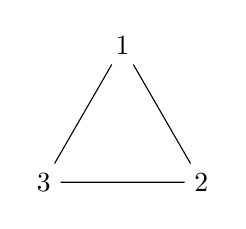
\begin{tikzpicture}
		\node (A) at (0,0) {3};
		\node (B) at (2,0) {2};
		\node (C) at (60:2) {1};
		\draw (A) -- (B) -- (C) -- (A);
	\end{tikzpicture}
\end{figure}

\paragraph*{角动量算符的本征态和本征值} 角动量$\boldsymbol{J}$的本征态和本征值如下
\begin{align}
	\boldsymbol{J}^2 |j\ m\rangle =& j(j+1)\hbar^2 |j\ m\rangle	\\
	J_z |j\ m\rangle =& m\hbar |j\ m\rangle
\end{align}
其正交性和归一性为
\begin{equation}
	\langle j^{\prime}\ m^{\prime} | j\ m\rangle = \delta_{jj^{\prime}}\delta_{mm^{\prime}}, \quad m = -j,\ -j+1, \ \cdots, j-1,\ j \ .
\end{equation}
此外,我们定义角动量的梯度算符
\begin{equation}
	J_{\pm} = J_{x} \pm i J_{y}
\end{equation}
满足对易式
\begin{equation}
	\left[J_{+}, J_{-}\right] = 2\hbar J_z, \quad \left[J_{\pm}, J_{z}\right] = \mp \hbar J_{\pm}
\end{equation}
梯度算符作用到本征态上的效果为
\begin{equation}
	\begin{aligned}
		J_{\pm} |j\ m\rangle =& \hbar \sqrt{j(j+1) - m(m\pm)1} |j\ m\pm 1\rangle	\\
						   =& \hbar \sqrt{(j\pm m +1) (j\mp m)} |j\ m\pm 1\rangle
	\end{aligned}
\end{equation}
对于单粒子在希尔伯特空间中的抽象角动量本征态$|j\ m\rangle$的坐标表示通常为\underline{球谐函数}。

%%%%%%%%%%%%%%%%%%%%%%%%%%%%%%%%%%%%%%%%%%%%%%%%%%%
%%%%%%%%%%%%%%%%%%%%%%%%%%%%%%%%%%%%%%%%%%%%%%%%%%%
\section{两角动量耦合与CG系数}
考虑两个完全对易的角动量$\boldsymbol{J}_1$和$\boldsymbol{J}_2$,也就是说这两个角动量分别属于两个不同的粒子,或者是一个粒子的自旋角动量和轨道角动量间的耦合。用CG系数表示耦合前和耦合后的角动量间关系。对于这样的两个角动量,我们有关系成立
\begin{equation}
	\left[\bmJ_1, \bmJ_2 \right] = 0 \quad
	\text{or}
	\quad
	\left[J_{1k}, J_{2l}\right] = 0,\ \text{for all}\ k, l = 1, 2, 3
\end{equation}

\paragraph*{CG系数} CG系数的解析表达式如下[\textit{Quantum Theory of Angular Momentum}, Eq. 8.2.1(3)]
\begin{equation}
    \begin{aligned}
        C_{j_1 m_1 j_2 m_2}^{j_3 m_3} 
        &= \delta_{m_3, m_1 + m_2} \Delta(j_1 j_2 j_3) \\
        \times& \left[ (j_1 + m_1)! (j_1 - m_1)! (j_2 + m_2)! (j_2 - m_2)! 
                 (j_3 + m_3)! (j_3 - m_3)!(2j_3 + 1)\right]^{1/2} \\
            \times& \sum_{k}\left[\frac{(-1)^k}{k!(j_1 + j_2 - j_3 - k)!(j_1 - m_1 - k)!
            (j_2 + m_2 - k)!(j_3 - j_2 + m_1 +k)!}\right.\\
                  &\left. \cdot \frac{1}{(j_3 - j_1 - m_2 + k)!} \right]
    \end{aligned}
    \label{eq:CG-representations}
\end{equation}
上式的$\Delta-symbol$定义如下
\begin{equation*}
    \Delta(j_1 j_2 j_3) = \left[ \frac{(j_1 + j_2 - j_3)! (j_1 - j_2 + j_3)! (-j_1 + j_2 + j_3)!}
                                      {(j_1 + j_2 + j_3 +1)!} \right]^{\frac{1}{2}}
\end{equation*}
其中,求和的上下限需保证所有阶乘项的自变量为非负,应满足一下条件
\begin{equation}
    \begin{aligned}
        k_{min} = \text{max} \left\{ 0, j_2 - m_1 - j_3, j_1 + m_2 - j_3 \right\}\\
        k_{max} = \text{min} \left\{ j_1 + j_2 - j_3, j_1 - m_1, j_2 + m_2 \right\}
    \end{aligned}
    \label{eq:CG-nonnegative}
\end{equation}



%%%%%%%%%%%%%%%%%%%%%%%%%%%%%%%%%%%%%%%%%%%%%%%%%%%

\chapter{转动及其他对称性算符}

\section{张量算符及Wigner-Eckart定理}

\subsection{Wigner-Eckart定理}
$T_{LM}$为$L$阶球张量,考虑这样一个量子态$\ket{\xi j m}$,角动量$j$及其第三分量$m$是好量子数,$\xi$包含了确定系统所需的其他所有量子数。这样,$T_{LM}$对应的矩阵元$\braket{\xi^{\prime} j^{\prime} m^{\prime} | T_{LM} | \xi j m}$可用Wigner-Eckart定理把角动量第三分量提取出来
\begin{equation}
    \boxed{
    \begin{aligned}
        \braket{\xi^{\prime} j^{\prime} m^{\prime} | T_{LM} | \xi j m}
        =& \hat{j^{\prime}}^{-1}\braket{jmLM | j^{\prime} m^{\prime}}
        \left(\xi^{\prime} j^{\prime} \| \bm{T}_{L} \| \xi j \right) \\
        =& (-1)^{j^\prime - m^\prime}
        \begin{pmatrix}
            j^{\prime} & L & j \\
            -m^{\prime}& M & m
        \end{pmatrix}
        \left(\xi^{\prime} j^{\prime} \| \bm{T}_{L} \| \xi j \right)      
    \end{aligned}
    }
    \label{eq:wigner-eckart}
\end{equation}
此处,$\left(\xi^{\prime} j^{\prime} \| \bm{T}_{L} \| \xi j \right)$为约化矩阵元,$\braket{\xi^{\prime} j^{\prime} m^{\prime} | T_{LM} | \xi j m}$为矩阵元。

\subsection{约化矩阵元的计算}
计算\cref{eq:wigner-eckart}定理中的约化矩阵元,只需取一些特定的值将左边的矩阵元算出,即可求出约化矩阵元。 




\part{原子核物理}
\chapter{原子核基本性质}

\section{原子核形状}
\paragraph*{核密度分布与核半径}
原子核作为一个多体量子体系,可以用多体波函数$\Psi(\bm{r})$来描述其基本性质。
原子核密度分布即多体波函数的平方
\begin{equation}
    \rho(\bm{r}) = | \Psi(\bm{r}) |^2   \label{eq:nucl.radius}
\end{equation}

\section{剩余相互作用}
\subsection{“对能”的简单理论模型}

\paragraph*{Seniority模型}
\CJKunderline{Seniority模型主要是针对满壳外的$j$壳层上的核子的处理}。在独立例子壳层模型中,不考虑对关联的原子核Hamiltonian的二次量子化形式为
\begin{equation}
    \hat{H}_{\text{独}}
        = \sum_{j} \varepsilon_j \sum_{m} \xi_{jm}^{\dagger} \xi_{jm}
    \label{eq:indep-hamil}
\end{equation}
其中,$\varepsilon_j$是$j$壳层的单粒子能量,$\xi_{jm}^{\dagger}$和$\xi_{jm}$对应为$\ket{jm}$态粒子的产生和湮灭算符。$\ket{jm}$态对应的粒子数算符为
\begin{equation}
    \hat{N}_{m} = \xi_{jm}^{\dagger} \xi_{jm}
\end{equation}
这样,$j$壳层所包含的粒子数算符写为
\begin{equation}
    \hat{N} = \sum_{m = -j}^{+j} \hat{N}_m
            = \sum_{m = -j}^{+j} \xi_{jm}^{\dagger} \xi_{jm}
\end{equation}
由于泡利原理,\CJKunderline{一个$\ket{jm}$态上只能有一个费米子(此处为核子)或者无粒子填充(即空穴)},因此$j$壳层的空穴数量为
\begin{equation}
    \sum_{m}(1 - \hat{N}_m) = \sum_{m}(1 -  \xi_{jm}^{\dagger} \xi_{jm} )
                    = \sum_{m}(\xi_{jm} \xi_{jm}^{\dagger} )
\end{equation}

由于$j$是单粒子自旋-轨道耦合的总角动量,因此总为半整数,故其对应的第三分量$m\neq 0$,引入配对粒子算符
\begin{equation}
    \hat{A}^{\dagger} = \sum_{m > 0} (-1)^{j - m} \xi_{jm}^{\dagger} \xi_{j-m}^{\dagger}
    \label{eq:def-pair}
\end{equation}
这里的$\pm m$表示全部量子数$n$、$l$、$j$、$\pm j_z$。算符$\hat{A}^{\dagger}$的意义是,它在$j$壳层同时产生一对核子,每个核子的角动量都为$j$,“配对”要求这两个核子耦合的总角动量$J = 0$。
\begin{proof}
    由\autoref{eq:def-pair},我们要求两个核子偶合成总角动量为0的态,因此耦合导致的CG系数为
    \begin{equation*}
        \Braket{jmj-m | 00} = (-1)^{j - m} \frac{\delta_{jj}\delta_{mm}}{\sqrt{2j + 1}}
    \end{equation*}
    这里用到了书籍\textit{Quantum Theory of Angular Momentum}中Section 8.5的Eq.\,(1)。
    这里出现了系数$(-1)^{j-m}$,但根号项尚未弄清楚,有可能吸到算符里了。
\end{proof}

对于偶数个费米子系统的集体算符,按玻色子的对易关系进行处理,上述配对算符是两费米子系统算符,因此使用玻色子对易关系
\begin{equation}
    [\hat{A}, \hat{A}^{\dagger}]_{-} = \left[\sum_{m > 0}(-1)^{j - m}\xi_{-m} \xi_{m}, \sum_{n > 0} (-1)^{j - m} \xi_{n}^{\dagger} \xi_{-n}^{\dagger}\right]_{-}
    \label{eq:fermi-pair-comm}
\end{equation}
\begin{note}
    \begin{equation*}
        \hat{A} = (\hat{A}^{\dagger})^{\dagger} = \sum_{m > 0} (-1)^{j - m} \xi_{jm}^{\dagger} (\xi_{j-m}^{\dagger})^{\dagger}
        = \sum_{m > 0} (-1)^{j - m} \xi_{j-m} \xi_{jm}
    \end{equation*}
\end{note}
利用费米子反对易关系,现在分以下情况考虑\Cref{eq:fermi-pair-comm}的关系:
\begin{enumerate}
    \item $n \neq m$时,有
        \begin{align*}
            \left[\xi_{-m} \xi_{m},\, \xi_{n}^{\dagger} \xi_{-n}^{\dagger}\right]_{-}
            =&\  \xi_{-m} \xi_{m} \xi_{n}^{\dagger} \xi_{-n}^{\dagger}
            - \xi_{n}^{\dagger} \xi_{-n}^{\dagger} \xi_{-m} \xi_{m}  \\
            =&\ \xi_{n}^{\dagger} \xi_{-n}^{\dagger} \xi_{-m} \xi_{m} 
            - \xi_{n}^{\dagger} \xi_{-n}^{\dagger} \xi_{-m} \xi_{m}  \\
            =&\ 0
        \end{align*}
    \item $n = m$时,有
        \begin{align*}
            \left[\xi_{-m} \xi_{m},\, \xi_{m}^{\dagger} \xi_{-m}^{\dagger}\right]_{-}
            =&\  \xi_{-m} \xi_{m} \xi_{m}^{\dagger} \xi_{-m}^{\dagger}
              - \xi_{m}^{\dagger} \xi_{-m}^{\dagger} \xi_{-m} \xi_{m}  \\
            =&\  \xi_{-m} (1 - \xi_{m}^{\dagger} \xi_{m}) \xi_{-m}^{\dagger}
              - \xi_{m}^{\dagger} \xi_{-m}^{\dagger} \xi_{-m} \xi_{m} \\
            =&\  \xi_{-m}\xi_{-m}^{\dagger} - \xi_{-m}\xi_{m}^{\dagger} \xi_{m} \xi_{-m}^{\dagger}
              - \xi_{m}^{\dagger} \xi_{-m}^{\dagger} \xi_{-m} \xi_{m} \\
            =&\  1 - \xi_{-m}^{\dagger}\xi_{-m} - \xi_{m}^{\dagger} \xi_{m} \xi_{-m} \xi_{-m}^{\dagger}
              - \xi_{m}^{\dagger} \xi_{-m}^{\dagger} \xi_{-m} \xi_{m} \\
            =&\  1 - \xi_{-m}^{\dagger}\xi_{-m} - \xi_{m}^{\dagger} \xi_{m} (1 - \xi_{-m}^{\dagger}\xi_{-m})
              - \xi_{m}^{\dagger} \xi_{-m}^{\dagger} \xi_{-m} \xi_{m} \\
            =&\  1 - \xi_{-m}^{\dagger}\xi_{-m} - \xi_{m}^{\dagger} \xi_{m} + \cancel{\xi_{m}^{\dagger} \xi_{m}\xi_{-m}^{\dagger}\xi_{-m}
              - \xi_{m}^{\dagger} \xi_{-m}^{\dagger} \xi_{-m} \xi_{m} } \\ 
            =&\  1 - \xi_{-m}^{\dagger}\xi_{-m} - \xi_{m}^{\dagger} \xi_{m}
        \end{align*}
\end{enumerate}
由以上分析,我们有关于配对粒子算符的对易关系
\begin{equation}
    \begin{aligned}
        \left[\hat{A},\, \hat{A}^{\dagger}\right]_{-}
        =& \sum_{m > 0}(1 - \xi_{-m}^{\dagger}\xi_{-m} - \xi_{m}^{\dagger} \xi_{m}) \\
        =&  \sum_{m > 0}(1 - N_{-m} - N_{m}) \\
        =& j + \frac{1}{2} - N
    \end{aligned}
\end{equation}
最后一步考虑到$m>0$的项一共有$j + \nicefrac{1}{2}$项(核子的总角动量$j$与其第三分量$m$为半整数),粒子数算符为$N = \sum_{m} N_{-m} + N_{m}$。

剩余相互作用是非常复杂的,现在只考虑核子间配对作用,由于是在独立粒子模型下引入的,因此核子配对算符应附加在\Cref{eq:indep-hamil}之后:
\begin{equation}
    \hat{H} = \hat{H}_{\text{独}} + \hat{H}_{\text{对}}
    = \sum_{j} \varepsilon_j \sum_{m} \xi_{jm}^{\dagger} \xi_{jm} - G\sum_{j}\hat{A}_{j}^{\dagger}\hat{A}_{j}
\end{equation}
\chapter{液滴模型}
%%%%%%%%%%%%%%%%%%%%%%%%%%%%%%%%%%%%%%%%%%%%%%%%%%%%%%%%%%%%%%%%%%%%%%%%%%%%%%%%%%
\section{引言}
\paragraph*{液滴模型(LDM)提出的依据}
\begin{enumerate}
	\item 原子核的不可压缩性:一般的,我们认为原子核无法的压缩性极低,且其体积不随其形状的改变而发生变化;
	\item 原子核具有明确的表面(well defined surface);
	\item 原子核中核力的\textcolor{red}{\underline{饱和性质:}}原子核中的一个核子仅与有限个核子发生相互作用。
\end{enumerate}

基于上面原子核的性质,人们提出了所谓的液滴模型,将原子核当成一个均匀带电的、不可压缩的、体积不变的液滴。从严格意义上来讲,这与真实的原子核情况是不相符的:原子核还具有结团(cluster)现象,表现为质量数等于4的核较为稳定;此外,在经典液滴中,两粒子的平均距离由粒子间作用力的极小值给出,大约为0.7fm,但是真实原子核应该是一个量子流体,其中的粒子间平均距离约为2.4fm,这是因为核子是满足费米统计(Fermi statistics)的,此时,泡利原理(Pauli principle)会阻止核子间距离过于接近,从而切掉了大部分两体力,导致核子间距离变大;在一个量子流体中是很少发生散射的,而在经典液滴中则以散射为主要反应。

\paragraph*{原子核的结合能}
对于一个包含$A$个粒子的系统,其结合能若只由两体力提供,那么它的总结合能$B(N,Z)$与粒子所构成的两体相互作用的组合数成正比关系,即有如下关系成立:
\begin{equation*}
	B(N, Z) \propto
	\begin{pmatrix}
		2	\\
		A
	\end{pmatrix}
	= \frac{1}{2} A(A-1)
\end{equation*} 
上述关系的例子可参考原子中的电子结合能。按上所述,原子核的总结合能$B(N,Z)$应随质量数的增大而增大,而且其\underline{\textcolor{red}{每核子的结合能}}(或称\underline{\textcolor{red}{比结合能}})应随质量数呈线性递增的关系,但实验发现对于质量数$A > 12$的原子核,其比结合能会大致处在某一常数附近
\begin{equation}
	\frac{B(N, Z)}{A} \simeq -8.5 [\text{ MeV/nucleon }]  \label{eq_specific_binding_energy}
\end{equation} 
原子核中结合能的行为可由核力的饱和性质进行解释。而这最后可归因到核力的短程性以及泡利原理与不确定性原理的结合。
\begin{note}
	核力是短程力的表现:核力的作用范围为$< 1.5 \times 10^{-15} {\rm m}$,在大于$0.8 \times 10^{-15} {\rm m}$ 时表现为吸引力,而且随着距离的增大而减小,当两核子距离$> 1.5 \times 10^{-15} {\rm m}$时核力会迅速降低并消失;两核子距离$ < 0.8 \times 10^{-15} {\rm m}$时,核力表现为排斥力,且随距离的减小而增大。
\end{note}

\paragraph*{原子核半径}
若将原子核描述为一个密度为常数并且具有sharp表面的球体,那么其半径可取经验公式
\begin{equation}
	R = r_0 A^{1/3}	\label{eq_nuclear_radius}
\end{equation} 
参数$r_0$一般取经验值$r_0 = 1.2 {\rm fm}$。

\paragraph*{原子核结合能的半经验公式:}根据液滴模型,C.F. Weizaker提出了原子核结合能的半经验公式:
\begin{equation}
	B(N, Z) = a_V A + a_S A^{2/3} + a_C \frac{Z^2}{A^{1/3}} + a_I \frac{(N-Z)^2}{A} - \delta(A)	\label{eq_semi-empirical_mass_formula}
\end{equation} 
其中拟合参数为
\begin{equation}
    \begin{aligned}
		a_V = -15.68; \quad a_S = 18.56; \quad a_C = 0.717; \quad a_I = 28.1	\quad	[MeV]	\\
		\delta(A) = \left\{ \begin{array}{cc}
				34 \cdot A^{-3/4} & \text{ for even-even } \\
				0 & \text{ for even-odd }	\\
				-34 \cdot A^{-3/4} & \text{ for odd-odd }
		\end{array}\right\} \text{nuclei}
    \end{aligned}
    	\label{eq_semi-empirical_mass_formula_fit}
\end{equation} 
式\eqref{eq_semi-empirical_mass_formula_fit}等号右边逐项的物理解释如下:
\begin{enumerate}
	\item 第一项:体积能项,因为$ A \propto R^3$,对应于球形的体积公式;
	\item 第二项:表面能项,因为$ A^{2/3} \propto R^2$,对应于球形面积公式;
	\item 第三项:库伦能项,表示质子间的库伦排斥项。库伦能正比于原子核中的质子对数量($\propto Z^2$),并与半径称反比。
	\item 第四项:对称能项,若没有泡利原理,由于质子间存在库仑斥力,因此原子核更倾向于仅包含中子的情况;
	\item 第五项:对能项,考虑到偶偶核、偶奇核、奇奇核的质量差等因素。
\end{enumerate}
得到结合能公式后的拟合图像如下图所示


\section{形变参数}
\paragraph*{形变原子核半径}
原子核的形状可体现在其表面上某一点到原点的距离,也就是形变核核中从原点到表面的半径矢量
\begin{equation}
	R = R(\theta, \phi) = R_0 ( 1 + \alpha_{00} + \sum_{\lambda = 1}^{\infty} \sum_{\mu = -\lambda}^{\lambda}\alpha^{*}_{\lambda\mu} Y_{\lambda\mu}(\theta, \phi) )	\label{eq:nul-radii}
\end{equation} 
其中$R_0$表示相同体积的球形核半径。此公式并非唯一描述该半径的公式,但却是最常用的。

%%%%%%%%
\section{球形核的表面振动}
原子核具有一些动力学特征,比如原子核整体的转动和振动等,当我们描述这些运动是,原子核的表面特征是一个动力学的过程。\Cref{eq:nul-radii}描述原子核的形状,其中$Y_{\lambda\mu}$具有固定表达,它是随时间不变的量。为描述原子核的动力学特征,我们可以将参数$\alpha_{\lambda\mu}$认为是随时间变化的量:$\alpha_{\lambda\mu}(t)$\citep[Sect. 1.4]{Peter2004}。

%%%%%%%%
\section{Bohr哈密顿量}
经典哈密顿量表述为(还未进行量子化前)
\begin{equation}
    H = \frac{1}{2} \sum_{\mathcal{K}}^{3} \mathcal{J}\omega_{\mathcal{K}}^2 + \frac{1}{2} D \left[\dot{\beta}^2 + \dot{\gamma}^2 \right] + V(\beta, \gamma)
	\label{eq:class-bohr-hamiltonian}
\end{equation}

\Cref{eq:class-bohr-hamiltonian}量子化后对应的动能项为
\begin{equation}
	T = \frac{1}{2} \sum_{\mathcal{K}}^{3} \mathcal{J}\omega_{\mathcal{K}}^2 + \frac{1}{2} D \left[\dot{\beta}^2 + \dot{\gamma}^2 \right]
	= \frac{1}{2} D \left[\dot{\beta}^2 + \dot{\gamma}^2 \right] + \frac{1}{2} \sum_{\mathcal{K}}^{3} \mathcal{J}\omega_{\mathcal{K}}^2
\end{equation}
其广义动量为$\dot{\beta}$,$\dot{\gamma}$和$\omega_{\mathcal{K}}$,共5个独立变量,故在度规$g_{ij}$中仅包含对角元
\begin{equation}
    \bm{G} = \begin{pmatrix}
		D & 0        & 0     & 0     & 0 \\
		0 & D\beta^2 & 0     & 0     & 0 \\
		0 & 0        & J_{1} & 0     & 0 \\
		0 & 0        & 0     & J_{2} & 0 \\
		0 & 0        & 0     & 0     & J_{3}
	\end{pmatrix}
\end{equation}

\begin{note}
笛卡尔坐标系下体系动能为$\cfrac{1}{2}\sum\limits_{i} \dot{x}_i^2$,其在曲线坐标系下表示为
\begin{equation}
	T = \frac{1}{2} \sum_{ij} g_{ij} \dot{q}_i \dot{q}_j
    \label{eq:curve-classical-kin}
\end{equation}
对应的动能变换矩阵为$\bm{G} = (g_{ij}) = \left(\sum\limits_{\alpha}\cfrac{\partial x_{\alpha}}{\partial q_i}\cfrac{\partial x_{\alpha}}{\partial q_j}\right)$,其逆矩阵为$\bm{G}^{-1} = (g^{-1}_{ij})$,对应的行列式为$|\bm{G}| = J^2$,我们现在对\cref{eq:curve-classical-kin}进行量子化。首先根据\cref{eq:mat-der-var,eq:det-log-dev},有以下方程成立
        \begin{equation*}\begin{aligned}
            \frac{d |\bm{G}|}{d q_{k}} =& 
            |\bm{G}| {\rm Tr} \left( \bm{G}^{-1} \frac{d \bm{G}}{d q_{k}} \right) \\
            \frac{\ln{|\bm{G}|}}{d q_{k}} =& \frac{1}{|\bm{G}|} \frac{d |\bm{G}|}{d q_{k}} = {\rm Tr} \left( \bm{G}^{-1} \frac{d \bm{G}}{d q_{k}} \right)
        \end{aligned}\end{equation*}
        这里已经假定$|\bm{G}| > 0$。定义矩阵
        \begin{equation*}
            \bm{D} = (d_{i\alpha}) = \left(\frac{\partial x_{i}}{\partial q_{\alpha}}\right), \quad \bm{D}^{-1} = (d^{-1}_{i\alpha}) = \left(\frac{\partial q_{i}}{\partial x_{\alpha}}\right)
        \end{equation*}
        这样,就有
        \begin{equation*}\begin{aligned}
            \bm{G} =& \bm{D}^{T}\bm{D} = (g_{ij}) = \left(\sum_{\alpha}d^{T}_{i\alpha}d_{\alpha j}\right) = \left(\sum_{\alpha}\frac{\partial x_{\alpha}}{\partial q_i}\frac{\partial x_{\alpha}}{\partial q_j}\right) \\
            \bm{G}^{-1} =& (g^{-1}_{ij}) = \bm{D}^{-1}\bm{D}^{T-1} = \left(\sum_{\alpha}\frac{\partial q_{i}}{\partial x_{\alpha}}\frac{\partial q_{j}}{\partial x_{\alpha}}\right) \\
        \end{aligned}\end{equation*}
以上可得
\begin{equation}\begin{aligned}
    \frac{\partial \ln{|\bm{G}|}}{\partial q_k} =& \frac{\partial \ln{(J^2)}}{\partial q_k} = 2 \frac{\partial \ln{J}}{\partial q_k} = 2 \frac{\partial \ln{|\bm{D}|}}{\partial q_k} =  2{\rm Tr} \left( \bm{D}^{-1} \frac{d \bm{D}}{d q_{k}} \right) \\
    =& 2\sum_{ij}d^{-1}_{ji}\frac{\partial d_{ij}}{\partial q_{k}} = 2 \sum_{ij}\frac{\partial q_{j}}{\partial x_{i}} \frac{\partial}{\partial q_{k}} \left(\frac{\partial x_{i}}{\partial q_j}\right) = 2 \sum_{ij}\frac{\partial q_{j}}{\partial x_{i}} \frac{\partial}{\partial q_{j}} \left(\frac{\partial x_{i}}{\partial q_k}\right)
\end{aligned}\end{equation}
注意到
\begin{equation}\begin{aligned}
    \sum_{ij}\left[\frac{\partial q_{j}}{\partial x_{i}} \frac{\partial}{\partial q_{j}} \left(\frac{\partial x_{i}}{\partial q_k}\right) + \frac{\partial x_{i}}{\partial q_k}\frac{\partial}{\partial q_{j}} \left(\frac{\partial q_{j}}{\partial x_{i}} \right)\right] =& \sum_{ij} \frac{\partial }{\partial q_{j}} \left(\frac{\partial q_{j}}{\partial x_{i}} \frac{\partial x_{i}}{\partial q_{k}}\right) \\
    =& \sum_{j}\frac{\partial }{\partial q_{j}} \left(\sum_{i} \frac{\partial q_{j}}{\partial x_{i}} \frac{\partial x_{i}}{\partial q_{k}}\right) \\
    =& \sum_{j}\frac{\partial }{\partial q_{j}} \left(\frac{d q_{j}}{d q_{k}}\right) \\
    =& \sum_{j}\frac{\partial }{\partial q_{j}} \delta_{jk} \\
    =& 0
\end{aligned}\end{equation}
这样,我们有
\begin{equation}
    \frac{\partial \ln{|\bm{G}|}}{\partial q_k} = -2\sum_{ij}\frac{\partial x_{i}}{\partial q_k} \left(\frac{\partial}{\partial q_{j}}\frac{\partial q_{j}}{\partial x_{i}} \right), \quad \frac{\partial \ln{J}}{\partial q_k} = -\sum_{ij}\frac{\partial x_{i}}{\partial q_k} \left(\frac{\partial}{\partial q_{j}}\frac{\partial q_{j}}{\partial x_{i}} \right)
\end{equation}
另外,从坐标$x_{i}$到坐标$q_{i}$,有
\begin{equation}\begin{aligned}
    \frac{\partial}{\partial x_{i}} =& \sum_{\alpha} \frac{\partial q_{\alpha}}{\partial x_{i}} \frac{\partial}{\partial q_{\alpha}} \\
    \sum_{i}\frac{\partial^{2}}{\partial x_{i} \partial x_{i}} =& \sum_{i \alpha\beta} \frac{\partial q_{\alpha}}{\partial x_{i}} \frac{\partial}{\partial q_{\alpha}} \left(\frac{\partial q_{\beta}}{\partial x_{i}} \frac{\partial}{\partial q_{\beta}}\right) \\
    =& \sum_{i \alpha\beta} \frac{\partial q_{\alpha}}{\partial x_{i}} \frac{\partial q_{\beta}}{\partial x_{i}} \frac{\partial^2}{\partial q_{\alpha}\partial q_{\beta}} + \frac{\partial q_{\alpha}}{\partial x_{i}}  \left(\frac{\partial}{\partial q_{\alpha}}\frac{\partial q_{\beta}}{\partial x_{i}}\right) \frac{\partial}{\partial q_{\beta}}\\
    =& \sum_{\alpha\beta} \frac{\partial q_{\alpha}}{\partial x_{i}} \frac{\partial q_{\beta}}{\partial x_{i}} \frac{\partial^2}{\partial q_{\alpha}\partial q_{\beta}} + \left(\frac{\partial}{\partial q_{\alpha}}\frac{\partial q_{\alpha}}{\partial x_{i}}\frac{\partial q_{\beta}}{\partial x_{i}}\right) \frac{\partial}{\partial q_{\beta}} - \frac{\partial q_{\beta}}{\partial x_{i}} \left(\frac{\partial}{\partial q_{\alpha}}\frac{\partial q_{\alpha}}{\partial x_{i}}\right) \frac{\partial}{\partial q_{\beta}} \\
    =& \sum_{\alpha\beta} \left[\left(\sum_{i}\frac{\partial q_{\alpha}}{\partial x_{i}} \frac{\partial q_{\beta}}{\partial x_{i}}\right) \frac{\partial^2}{\partial q_{\alpha}\partial q_{\beta}} + \left(\frac{\partial}{\partial q_{\alpha}} \left(\sum_{i}\frac{\partial q_{\alpha}}{\partial x_{i}}\frac{\partial q_{\beta}}{\partial x_{i}}\right)\right) \frac{\partial}{\partial q_{\beta}} - \sum_{i}\frac{\partial q_{\beta}}{\partial x_{i}} \left(\frac{\partial}{\partial q_{\alpha}}\frac{\partial q_{\alpha}}{\partial x_{i}}\right) \frac{\partial}{\partial q_{\beta}}\right] \\
    =& \sum_{\alpha\beta} \left(g^{-1}_{\alpha\beta} \frac{\partial^2}{\partial q_{\alpha}\partial q_{\beta}} + \frac{\partial g^{-1}_{\alpha\beta}}{\partial q_{\alpha}} \frac{\partial}{\partial q_{\beta}}\right) - \sum_{i\alpha\beta}\frac{\partial q_{\beta}}{\partial x_{i}} \left( \frac{\partial}{\partial q_{\alpha}}\frac{\partial q_{\alpha}}{\partial x_{i}}\right) \frac{\partial}{\partial q_{\beta}}
\end{aligned}\end{equation}
同时,我们注意到
\begin{equation}\begin{aligned}
    \sum_{ij}\frac{1}{J} \frac{\partial}{\partial q_{i}}{g}^{-1}_{ij} J \frac{\partial}{\partial q_j} =& \sum_{ij}\frac{1}{J} \left[{g}^{-1}_{ij} J \frac{\partial^2}{\partial q_{i}\partial q_{j}} + \frac{\partial ({g}^{-1}_{ij}J)}{\partial q_{i}} \frac{\partial}{\partial q_{j}}\right] \\
    =& \sum_{ij}{g}^{-1}_{ij} \frac{\partial^2}{\partial q_{i}\partial q_{j}} + \frac{\partial {g}^{-1}_{ij}}{\partial q_{i}} \frac{\partial}{\partial q_{j}} + {g}^{-1}_{ij}\frac{1}{J}\frac{\partial J}{\partial q_{i}} \frac{\partial}{\partial q_{j}} \\
    =& \sum_{ij}{g}^{-1}_{ij} \frac{\partial^2}{\partial q_{i}\partial q_{j}} + \frac{\partial {g}^{-1}_{ij}}{\partial q_{i}} \frac{\partial}{\partial q_{j}} + {g}^{-1}_{ij}\frac{\partial \ln{J}}{\partial q_{i}} \frac{\partial}{\partial q_{j}}
    \label{eq:expand1}
\end{aligned}\end{equation}
这里的最后一项展开
\begin{equation}\begin{aligned}
    \sum_{ij}{g}^{-1}_{ij}\frac{\partial \ln{J}}{\partial q_{i}} \frac{\partial}{\partial q_{j}} =& -\sum_{ij} {g}^{-1}_{ij} \left(\sum_{\alpha k}\frac{\partial x_{\alpha}}{\partial q_{i}} \frac{\partial}{\partial q_{k}} \frac{\partial q_{k}}{\partial x_{\alpha}}\right) \frac{\partial}{\partial q_{j}} \\
    =& -\sum_{ij}\left(\sum_{\beta}\frac{\partial q_{i}}{\partial x_{\beta}} \frac{\partial q_{j}}{\partial x_{\beta}}\right) \left(\sum_{\alpha k}\frac{\partial x_{\alpha}}{\partial q_{i}} \frac{\partial}{\partial q_{k}} \frac{\partial q_{k}}{\partial x_{\alpha}}\right) \frac{\partial}{\partial q_{j}} \\
    =& -\sum_{j\alpha\beta k}\left(\sum_{i}\frac{\partial x_{\alpha}}{\partial q_{i}}\frac{\partial q_{i}}{\partial x_{\beta}}\right)  \frac{\partial q_{j}}{\partial x_{\beta}} \left(\frac{\partial}{\partial q_{k}} \frac{\partial q_{k}}{\partial x_{\alpha}}\right) \frac{\partial}{\partial q_{j}} \\
    =& -\sum_{j\alpha\beta k} \frac{d x_{\alpha}}{d x_{\beta}} \frac{\partial q_{j}}{\partial x_{\beta}} \left(\frac{\partial}{\partial q_{k}} \frac{\partial q_{k}}{\partial x_{\alpha}}\right) \frac{\partial}{\partial q_{j}} \\
    =& -\sum_{j\alpha\beta k} \delta_{\alpha\beta} \frac{\partial q_{j}}{\partial x_{\beta}} \left(\frac{\partial}{\partial q_{k}} \frac{\partial q_{k}}{\partial x_{\alpha}}\right) \frac{\partial}{\partial q_{j}} \\
    =& -\sum_{j\alpha k} \frac{\partial q_{j}}{\partial x_{\alpha}} \left(\frac{\partial}{\partial q_{k}} \frac{\partial q_{k}}{\partial x_{\alpha}}\right) \frac{\partial}{\partial q_{j}}
    \label{eq:expand2}
\end{aligned}\end{equation}
将\cref{eq:expand2}代回\cref{eq:expand1}并变换哑指标$k\rightarrow i$,最后得到
\begin{equation}\begin{aligned}
    \sum_{ij}\frac{1}{J} \frac{\partial}{\partial q_{i}}{g}^{-1}_{ij} J \frac{\partial}{\partial q_j} = \sum_{ij}\left({g}^{-1}_{ij} \frac{\partial^2}{\partial q_{i}\partial q_{j}} + \frac{\partial {g}^{-1}_{ij}}{\partial q_{i}} \frac{\partial}{\partial q_{j}} \right) - \sum_{ij\alpha}\left(\frac{\partial q_{j}}{\partial x_{\alpha}} \left(\frac{\partial}{\partial q_{i}} \frac{\partial q_{i}}{\partial x_{\alpha}}\right) \frac{\partial}{\partial q_{j}}\right)
\end{aligned}\end{equation}
以上,可知量子化后的动能想可表述为
\begin{equation}
	\hat{T} = -\frac{\hbar^2}{2} \sum_{ij} |g^{-1/2}| \frac{\partial}{\partial \q_i} |g^{1/2}| g^{-1}_{ij} \frac{\partial}{\partial \q_{j}}
\end{equation}
\end{note}


\bibliographystyle{modified-apsrev4-2}
\bibliography{reference}

\include{contents/nuclear/mfc}
\chapter{原子核平均场及多核子组态}

本章主要参考\citet[][Chap. 3]{suhonen-NtoN}。
\section{原子核平均场}

%%%%%%%%%%%%
\paragraph*{准粒子} 准粒子一般用来作为粒子近似。准粒子系统可以当成无相互作用的准粒子进行处理。

%%%%%%%%%%%%
\paragraph*{平均场近似} 
平均场处理方法如下:
\begin{enumerate}
	\item 质量数$A$,质子数$Z$,中子数$N$,满足$A=N+Z$;
	\item 把核子当成没有内部结构的点粒子;
	\item 核子间的强相互作用(核力)转换到弱相互作用或无相互作用的准粒子系统;
	\item 余下的核子间相互作用称为剩余相互作用,将使用微扰理论进行处理。
\end{enumerate}

平均场近似下,复杂的多体相互作用将被忽略。一般认为一个核子与其它$A-1$个核子间发生两体相互作用,类似瞬时力的概念,核子间的相互作用势场可理解为无穷小时间间隔内的核子-核子相互作用的平均
\begin{equation}
	v(\bm{r}_i) = \frac{1}{\Delta T} \int_{T}^{T + \Delta T} dt\, \sum_{j = 1; j \neq i}^{A} v(\bm{r}_i(t), \bm{r}_j(t))
\end{equation}
这样,原子核的平均场被认为由这$A$个粒子所受的势场所组成
\begin{equation}
	V_{mf} = \sum_{i}^{A} v(\bm{r}_i)
\end{equation}
核子将在上式所示的势场中运动。

以下将讨论所谓的平均场(或Hartree-Fock)准粒子。在像原子核这样的多体系统中,核子-核子相互作用可忽略掉三体及以上的多体相互作用,最高写成两体相互作用的形式,其哈密顿量由动能项和势能项组成:
\begin{equation}
	H = T + V = \sum_{i = 1}^{A} t(\bm{r}_i) + \sum_{i, j = 1; i < j}^{A} v(\bm{r}_i, \bm{r}_j) =  \sum_{i = 1}^{A} \frac{-\hbar^2}{2m_N}\nabla_i^2 + \sum_{i, j = 1; i < j}^{A} v(\bm{r}_i, \bm{r}_j) 
\end{equation}
$m_N$表示核子质量(这里假设中子和质子具有相同的核子质量$m_N c^2 \approx 940\, \rm{MeV}$),$\bm{r}_i$表示第$i$个核子的坐标。
可以加上减去这个单粒子势能,有
\begin{equation}
	H = \left[T + \sum_{i}^{A}v(\bm{r}_i) \right] + \left[V - \sum_{i}^{A} v(\bm{r}_i)\right]
	= H_{mf} + H_{res}
\end{equation}
其中,定义\CJKunderline{原子核平均场哈密顿量}为
\begin{equation}
	H_{mf} = T + \sum_{i}^{A} v(\bm{r}_i) = \sum_{i}^{A}\left[t(\bm{r}_i) + v(\bm{r}_i)\right] \equiv \sum_{i}^{A} h(\bm{r}_i)
	\label{eq:mf-hamil}
\end{equation}
\CJKunderline{原子核剩余相互作用比初始势能$V$小得多,}定义为
\begin{equation}
	V_{res} = V - \sum_{i}^{A} v(\bm{r}_i) \equiv \sum_{i, j = 1; i < j}^{A} v(\bm{r}_i, \bm{r}_j) - \sum_{i}^{A}v(\bm{r}_i)
\end{equation}

%%%%%%%%%%%%
\paragraph*{原子核集体波函数$\Psi_0$的理解:}在\uline{\textsl{Hartree}}方法中,集体波函数
只表现为单粒子态的直积形式,如下
\begin{equation}
	\Psi_0(\bm{r}_1,\ \bm{r}_2,\ \bm{r}_3,\cdots,\ \bm{r}_A) = \prod_{i=1}^{A} 
    \phi_{\alpha_i}(\bm{r}_i)
\end{equation} 
在\uline{\textsl{Hartree-Fock}}方法中,集体波函数表现为单粒子波函数直积形式的混合,且具有反
对称性质,如下
\begin{equation}
    \begin{aligned}
		\Psi_0(\bm{r}_1, \bm{r}_2, \bm{r}_3, \cdots, \bm{r}_A) ={}& \mathcal{A}\left[ 
        \prod_{i=1}^{A} \phi_{\alpha_i}(\bm{r}_i) \right]	\\
		={}& 
		\begin{vmatrix}
			\phi_1(\bm{r}_1)	&	\phi_1(\bm{r}_2)	&	\phi_1(\bm{r}_3)	&	\cdots	&	\phi_1(\bm{r}_A)	\\
			\phi_2(\bm{r}_1)	&	\phi_2(\bm{r}_2)	&	\phi_2(\bm{r}_3)	&	\cdots	&	\phi_2(\bm{r}_A)	\\
			\phi_3(\bm{r}_1)	&	\phi_3(\bm{r}_2)	&	\phi_3(\bm{r}_3)	&	\cdots	&	\phi_3(\bm{r}_A)	\\
			\vdots				&	\vdots				&	\vdots				&	\ddots	&	\vdots				\\
			\phi_A(\bm{r}_1)	&	\phi_A(\bm{r}_2)	&	\phi_A(\bm{r}_3)	&	\cdots	&	\phi_A(\bm{r}_A)	\\
		\end{vmatrix}
    \end{aligned}
\end{equation} 
	其中,$\mathcal{A}$为反对称化算符,并且包含了归一化系数;$\bm{r}_1,\ \bm{r}_2,\ \cdots,
    \ \bm{r}_A$表示粒子$1,\ 2,\ \cdots,\ A$的坐标;$\phi_1,\ \phi_2,\ \cdots,\ \phi_A$表
    示有那么多个能级,也就是粒子可能占据的能级。我们现在考虑三粒子体系的情况,三个粒子占
    据三个能级,在\textsl{Hartree-Fock}方法中,其集体波函数可表示为
\begin{equation}
    \begin{aligned}
		\Psi_0(\bm{r}_1, \bm{r}_2, \bm{r}_3) ={}& \mathcal{A}\left[ \prod_{i=1}^{3} 
        \phi_{\alpha_i}(\bm{r}_i) \right]	\\
		={}& \frac{1}{\sqrt{6}} 
		\begin{vmatrix}
			\phi_1(\bm{r}_1)	&	\phi_1(\bm{r}_2)	&	\phi_1(\bm{r}_3)	\\
			\phi_2(\bm{r}_1)	&	\phi_2(\bm{r}_2)	&	\phi_2(\bm{r}_3)	\\
			\phi_3(\bm{r}_1)	&	\phi_3(\bm{r}_2)	&	\phi_3(\bm{r}_3)	\\
		\end{vmatrix}	\\
		=& \frac{1}{\sqrt{6}} \left[\phi_1(\bm{r}_1)\phi_2(\bm{r}_2)\phi_3(\bm{r}_3) + \phi_1(\bm{r}_2)\phi_2(\bm{r}_3)\phi_3(\bm{r}_1) + \phi_1(\bm{r}_3)\phi_2(\bm{r}_1)\phi_3(\bm{r}_2)\right. \\
		& \left. - \phi_1(\bm{r}_3)\phi_2(\bm{r}_2)\phi_3(\bm{r}_1) - \phi_1(\bm{r}_2)\phi_2(\bm{r}_1)\phi_3(\bm{r}_3) - \phi_1(\bm{r}_1)\phi_2(\bm{r}_3)\phi_3(\bm{r}_2)\right] 
    \end{aligned}
\end{equation} 
现在我们考察上式第二个等号的左边第一项,$\phi_1(\bm{r}_1)\phi_2(\bm{r}_2)\phi_3(\bm{r}_3)$表示粒子$1$处于能级$\phi_1$、位置在$\bm{r}_1$,且粒子$2$处于能级$\phi_2$、位置在$\bm{r}_2$,同时粒子$3$处于能级$\phi_3$、位置在$\bm{r}_3$的概率;后面几项类同。事实上,由于全同粒子的不可区分性,我们根本无法辨别粒子$1$、$2$、$3$,因此我们无法判断具体某一个态上的粒子具体是$1$、$2$、$3$中的哪一个,所以我们需要把各种情况考虑进来,同时考虑费米子的交换反对称性应加上对应的相位,上式最后一个等号右边的排列情况构成了如图\ref{fig:three-body-wv}所示:
\begin{figure}[htbp]
	\centering
	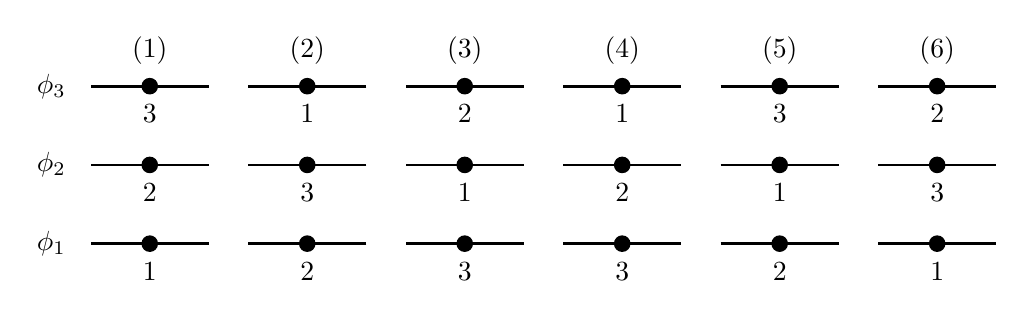
\begin{tikzpicture}
    \node at (-6.25, 2) {$\phi_3$};
    \node at (-6.25, 1) {$\phi_2$};
    \node at (-6.25, 0) {$\phi_1$};

    \node at (-5, 2.45) {(1)};
    \draw[line width=1pt] (-4.25, 2) -- (-5.75, 2);
    \draw[line width=1pt] (-4.25, 1) -- (-5.75, 1);
    \draw[line width=1pt] (-4.25, 0) -- (-5.75, 0);
    \fill (-5, 0)circle(3pt) (-5, 1)circle(3pt) (-5, 2)circle(3pt);
    \node at (-5, -0.35) {$1$};
    \node at (-5,  0.65) {$2$};
    \node at (-5,  1.65) {$3$};

    \node at (-3, 2.45) {(2)};
    \draw[line width=1pt] (-2.25, 2) -- (-3.75, 2);
    \draw[line width=1pt] (-2.25, 1) -- (-3.75, 1);
    \draw[line width=1pt] (-2.25, 0) -- (-3.75, 0);
    \fill (-3, 0)circle(3pt) (-3, 1)circle(3pt) (-3, 2)circle(3pt);
    \node at (-3, -0.35) {$2$};
    \node at (-3,  0.65) {$3$};
    \node at (-3,  1.65) {$1$};

    \node at (-1, 2.45) {(3)};
    \draw[line width=1pt] (-0.25, 2) -- (-1.75, 2);
    \draw[line width=1pt] (-0.25, 1) -- (-1.75, 1);
    \draw[line width=1pt] (-0.25, 0) -- (-1.75, 0);
    \fill (-1, 0)circle(3pt) (-1, 1)circle(3pt) (-1, 2)circle(3pt);
    \node at (-1, -0.35) {$3$};
    \node at (-1,  0.65) {$1$};
    \node at (-1,  1.65) {$2$};

    \node at (1, 2.45) {(4)};
    \draw[line width=1pt] (0.25, 2) -- (1.75, 2);
    \draw[line width=1pt] (0.25, 1) -- (1.75, 1);
    \draw[line width=1pt] (0.25, 0) -- (1.75, 0);
    \fill (1, 0)circle(3pt) (1, 1)circle(3pt) (1, 2)circle(3pt);
    \node at (1, -0.35) {$3$};
    \node at (1,  0.65) {$2$};
    \node at (1,  1.65) {$1$};

    \node at (3, 2.45) {(5)};
    \draw[line width=1pt] (2.25, 2) -- (3.75, 2);
    \draw[line width=1pt] (2.25, 1) -- (3.75, 1);
    \draw[line width=1pt] (2.25, 0) -- (3.75, 0);
    \fill (3, 0)circle(3pt) (3, 1)circle(3pt) (3, 2)circle(3pt);
    \node at (3, -0.35) {$2$};
    \node at (3,  0.65) {$1$};
    \node at (3,  1.65) {$3$};

    \node at (5, 2.45) {(6)};
    \draw[line width=1pt] (4.25, 2) -- (5.75, 2);
    \draw[line width=1pt] (4.25, 1) -- (5.75, 1);
    \draw[line width=1pt] (4.25, 0) -- (5.75, 0);
    \fill (5, 0)circle(3pt) (5, 1)circle(3pt) (5, 2)circle(3pt);
    \node at (5, -0.35) {$1$};
    \node at (5,  0.65) {$3$};
    \node at (5,  1.65) {$2$};
\end{tikzpicture}
	\caption{三粒子填充三条能级的体系集体波函数情况}
	\label{fig:three-body-wv}
\end{figure}

%%%%%%%%%%%%
\paragraph*{平均场的迭代求解}
平均场哈密顿量$H_{mf}$作用到$A$核子的集体波函数$\Psi_0(\bm{r}_1, \bm{r}_2, \cdots, \bm{r}_A)$上可得到原子核的总能量,得到相应的Sch{\"o}dinger方程
\begin{equation}
	H_{mf} \Psi_0 = E \Psi_0
	\label{eq:mf-scho-eq}
\end{equation}
由\cref{eq:mf-hamil},原子核集体波函数分写成单粒子波函数的直乘形式
\begin{equation}
	\Psi_0(\bm{r}_1, \bm{r}_2, \cdots, \bm{r}_A) = \phi_{\alpha_1}(\bm{r}_1) \phi_{\alpha_2}(\bm{r}_2) \cdots \phi_{\alpha_A}(\bm{r}_A)
	\label{def:collect-wv}
\end{equation}
$\phi_{\alpha_{i}}$表示不同能级上的单粒子波函数。

由\cref{eq:mf-hamil,eq:mf-scho-eq,def:collect-wv},平均场下的\textsl{Hartree(-Fock)}方程如下(表示单个粒子的类Sch{\"o}dinger方程):
\begin{equation}\boxed{
    \begin{aligned}
        \frac{-\hbar^{2}}{2m_N} \nabla^{2} \phi_{\alpha}(\bm{r}) + V_{H(F)}\left(
        \{\phi_{i}(\bm{r})\}\right)\phi_{\alpha} = \varepsilon_{\alpha}\phi_{\alpha}(\bm{r}) \\ 
        i = 1, 2, \cdots, A, \quad \alpha = 1, 2, \cdots, \infty
    \end{aligned}
    \label{eq:Hartree-Fock}
}\end{equation}
原子核能量为单粒子能量之和
\begin{equation}
	E = \sum_{i = 1}^{A} \varepsilon_{\alpha_i}
\end{equation}
$\varepsilon_{\alpha_i}$表示第$i$个粒子所在能级对应的能量。

\Cref{eq:Hartree-Fock}与Sch{\"o}dinger方程唯一不同就是势能变成了关于波函数的非线性函数,
\begin{equation*} V(\bm{r}) \Longrightarrow V_{H(F)}(\{\phi_{i}(\bm{r})\})
\end{equation*}
\Cref{eq:Hartree-Fock}为非线性方程组,一般用迭代的方法求解。我们先猜测得到一组试探
波函数$\{\phi_i^0(\bm{r})\}_{i=1}^{A}$,然后我们根据势能与波函数的关系得到初始势场
$V_{H(F)}^{0}$;完成上述步骤后,我们将试探波函数和初始势场带入\cref{eq:Hartree-Fock},
求解得到一组新的波函数$\{\phi_{\alpha}^1(\bm{r})\}_{\alpha=1}^{A}$和本征值$\varepsilon_{\alpha}^{(1)}$,
通过这组新的波函数,我们可以再次生成一个新的势场$V_{H(F)}^{(1)}$;将生成的新势场和新波函数
再次代入式\eqref{eq:Hartree-Fock},可得到更新一组的本征波函数和本征能量。通过比较某次迭代
前后的波函数间的误差小于某一给定值来确定波函数合理
\begin{equation}
    \parallel \phi_{\alpha}^{(n-1)} - \phi_{\alpha}^{(n)} \parallel < \text{preset limit}
    \label{eq:iter-error}
\end{equation}
其中,$\parallel \cdots \parallel$表示波函数的模。

此方法得到的势场一般为中心势场,只适合描述球形核。对于形变核需要进行额外的处理。

\paragraph*{关于平均势场和初始波函数形式的选取}
上述平均场方程中,势能具体形式为\citep[][Eqs. C2.3 and C2.6]{ningpz}
\begin{equation}\boxed{\begin{aligned}
    V_{H}\left( \left\{ \phi_i(\bm{r}) \right\} \right) \phi_j(\bm{r}_j) &= \sum_{i \neq j} \int 
    \phi_i^{\star}(\bm{r}_i^{\prime}) V_{ij}(\bm{r}_i^{\prime}, \bm{r}_j) \phi_{i}(\bm{r}_i^{\prime})
    \,d\bm{r}_i^{\prime}\ \phi_j(\bm{r}_j) \\
	V_{HF}\left( \left\{ \phi_i(\bm{r}) \right\} \right) \phi_j(\bm{r}_j) &= \sum_{i} \int 
    \phi_i^{\star}(\bm{r}_i^{\prime}) V_{ij}(\bm{r}_i^{\prime}, \bm{r}_j) \phi_{i}(\bm{r}_i^{\prime}) \phi_j(\bm{r}_j) - \phi_i^{\star}(\bm{r}_i^{\prime}) V_{ij}(\bm{r}_i^{\prime}, \bm{r}_j) \phi_{i}(\bm{r}_j) \phi_j(\bm{r}_i^{\prime})
    \,d\bm{r}_i^{\prime}  
    \label{eq:mean-field}
\end{aligned}}\end{equation}
为寻找到一组合适的平均场,试探波函数可以选取一组零级近似,如费米气体模型单粒子波函数:
\begin{equation}
    \phi_i = \sqrt{V^{-1}} \exp{(i \bm{k}_i \cdot \bm{r}_i)}
    \label{eq:fermi-gas-eigen}
\end{equation}
其中,$V$表示原子核的体积。对于二体势$V_{ij}$,可以选用Skyrme力(见下式)或其它形式的两体力
\begin{equation}
    V_{skyrme} = \sum_{i<j} v(i, j) + \sum_{i<j<k} v(i, j, k)
    \label{eq:skyrme-forc}
\end{equation}
其中,两体力部分为
\begin{equation}
    \begin{aligned}
        v(1, 2) =& t_0 (1 + x_0 P_{\sigma})\delta(\bm{r}_1 - \bm{r}_2) \\
            & + t_1\left[ \delta(\bm{r}_1 - \bm{r}_2) \bm{k}^{2}
              + \bm{k}^{\prime 2}\delta(\bm{r}_1 - \bm{r}_2)\right] / 2 \\
            & + t_2\bm{k}^{\prime} \cdot \delta(\bm{r}_1 - \bm{r}_2) \bm{k} \\
            & + {\rm i} W_0(\bm{\sigma}_1 + \bm{\sigma}_2)\cdot \left[ 
            \bm{k}^{\prime} \times \delta\left( \bm{r}_1 - \bm{r}_2 \right) \bm{k}\right]
    \end{aligned}
    \label{eq:skyrme-tow-body-forc}
\end{equation}
三体部分为
\begin{equation}
    v(1, 2, 3) = t_3 \delta(\bm{r}_1 - \bm{r}_2) \delta(\bm{r}_2 - \bm{r}_3)
    \label{eq:skyrm-three-body-forc}
\end{equation}
式中,$\bm{k} = \bm{p}/\hbar = (\nabla_{1} - \nabla_{2}) / (2{\rm i})$是向右作用的相对动量
算符,$\bm{k}^{\prime} = \bm{p}/\hbar = (\nabla_{2} - \nabla_{1}) / (2{\rm i})$是向左相对
动量算符;$P_{\sigma} = (1 + \bm{\sigma}_1 \cdot \bm{\sigma}_2) / 2$是自旋交换算符。上式
Skyrme力有6个可调参数$t_0$、$t_1$、$t_2$、$t_3$、$x_0$和$W_0$。

%%%%%%%%%%%%
\paragraph*{唯象势}
一般地,可以选取合适的势场作为固定的原子核集体势场,不需要进行迭代求解,这样选取的势场称为\CJKunderdot{唯象势}。唯象势使对原子核的计算更加简单,但会带来计算上的误差。
常用的两种唯象势
\begin{enumerate}
	\item 三维谐振子势
		\begin{equation}
			v_{ho}(r) = -V_1 + k r^2 = -V_1 + \frac{1}{2} m_N \omega r^2
		\end{equation}
		$V_1$和$k$由实验拟合。
	\item Woods-Saxon势
		\begin{equation}
			v_{ws}(r) = \frac{-V_0}{1 + e^{(r-R)/a}}
		\end{equation}
	一般的取值为
	\begin{equation}
		\begin{aligned}
			R = r_0 A^{\frac{1}{3}} = 1.27  A^{\frac{1}{3}}\ \rm{fm} \quad (nuclear radius) \\
			a = 0.67\ \rm{fm} \quad (surface diffuseness) \\
			V_0 = \left(55 \pm 33 \frac{N - Z}{A}\right) \ \rm{MeV}
		\end{aligned}
	\end{equation}
	质子取$+$,中子取$-$,当不区分核子时取$V_0 = 57\,\rm{MeV}$。
\end{enumerate}


%%%%%%%%%%%%%%%%%%%%%%%%%%%%%
\section{Woods-Saxon波函数}
基于以上给出的唯象Woods-Saxon势,并结合库伦势和自旋-轨道耦合作用,可以对原子核的类Sch{\"o}dinger方程进行数值求解,并将波函数在谐振子基下展开。

\paragraph*{单核子哈密顿量}
单核子薛定谔方程中的哈密顿量为:
\begin{equation}
	\begin{aligned}
		h =&\, \frac{-\hbar^2}{2 m_{N}} \nabla^2 + v(r) + v_{LS}(r) \bm{L}\cdot \bm{S}	\\
		=&\, \frac{-\hbar^2}{2 m_{N}}\left(\nabla^2_{r} - \frac{\bm{L}^2/\hbar^2}{r^2}\right) + v_{WS}(r) + v_{C}(r) + v_{LS}(r)\boldsymbol{L\cdot S}
	\end{aligned}
\end{equation} 
其中,径向偏分取一般形式
\begin{equation}
	\nabla^2_{r} \equiv \frac{1}{r^2} \frac{d}{dr} \left(r^2 \frac{d}{dr}\right)
\end{equation}
表示径向动能;括号中的第二项为核子“离心势能”项,它使系统总能量降低(所谓“向心力”是由势场提供的,核子的转动越大,它就有更大的能量脱离原子核,也就是离心势);$v_{WS}$是唯象Woods-Saxon势;$v_{C}(r)$为库伦势,只表示质子间的相互作用,若为中子,该项取0,原子核半径内取均匀带电的球静态库伦势,可得方程如下
\begin{equation}
	v_{C} = \frac{Ze^2}{4\pi\epsilon_0} \left\{
		\begin{aligned}
			&\frac{3 - (r/R)^2}{2R}, \quad & r\leqslant  R \\
			&\frac{1}{r}, \quad            & r > R  
		\end{aligned}
	\right.
\end{equation}
自旋-轨道耦合项系数为
\begin{equation}
	v_{LS}(r) = v_{LS}^{(0)} \left(\frac{r_0}{\hbar}\right)^2 \frac{1}{r} \left[\frac{d}{dr} \frac{1}{1 + e^{(r-R)/a}}\right]
	\label{eq:spin-orbit-der-term}
\end{equation}
中括号的偏分表示不作用到波函数上,并且这个偏分将使自旋-轨道耦合的峰位处于原子核表面区域。
\begin{example}[自旋-轨道耦合偏分项]
	假设原子核质量数$A = 100$,则对应的半径为$R = 1.27 \times 100^{\nicefrac{1}{3}} \approx 5.895\, \rm{fm}$,则\Cref{eq:spin-orbit-der-term}中的偏分项$f = \frac{d}{dr} \frac{1}{1 + e^{(r-5.895)/0.67}}$的图像如\Cref{fig:spin-orbit-der-term}
	\begin{figure}[htbp]
		\centering
		\includegraphics[scale=0.6]{figure/nuclear/spin-orbit-der.pdf}
		\caption{自旋轨道耦合偏分项}
		\label{fig:spin-orbit-der-term}
	\end{figure}
	可见,在原子核表面区域确实存在一个峰值,这表明原子核表面处自旋轨道耦合作用最强。
\end{example}
自旋-轨道耦合中的半径依赖通常可以用一个常数取代,我们取强度
\begin{equation}
	v_{LS}^{(0)} = 0.44 V_0
\end{equation}

\paragraph*{波函数用谐振子基展开}
三维谐振子波函数构成一组正交基,Woods-Saxon势下的原子核单粒子波函数可用这组谐振子基进行展开:
\begin{equation}
	f_{nlj}(r) = \sum_{\nu} A_{\nu}^{(nlj)} g_{\nu l}(r), \quad \sum_{\nu} [A_{\nu}^{(nlj)}]^2 = 1
\end{equation}
这样得到的核单核子波函数的细节见\Cref{sec:mat-diag}。

\paragraph*{Woods-Saxon哈密顿量的对角化}
得到球谐振子波函数后,可将这些波函数作为基矢展开构成Woods-Saxon势下的原子核波函数。谐振子展开的Woods-Saxon径向哈密顿量矩阵元为
\begin{equation}
    \begin{aligned}
		\langle \nu^{\prime} | h_{lj}(r) | \nu\rangle =&\int_{0}^{\infty} r^2 \,dr g_{\nu^{\prime} l}^{\ast}(r) g_{\nu l}(r) \left[ \frac{\hbar^2}{2m_N} \left(\frac{4n + 2l + 3}{b^2} - \frac{r^2}{b^4}\right) \right. \\
		&+ \left. v_{WS}(r) + v_{C}(r) + \frac{1}{2}\left[j(j+1) - l(l+1) - \frac{3}{4}\hbar^2 v_{LS}(r)\right] \right]
    \end{aligned}
\end{equation}
这样,整个矩阵就可以写成如下形式
\begin{equation}
	\begin{bmatrix}
		\langle 0 | h_{lj}(r) | 0 \rangle & \langle 0 | h_{lj}(r) | 1 \rangle & \cdots	& \cdots	\\
		\langle 1 | h_{lj}(r) | 0 \rangle & \langle 1 | h_{lj}(r) | 1 \rangle & \cdots	& \cdots	\\
		\vdots	&	\vdots	& \ddots & \vdots \\
		\cdots	&	\cdots	& \cdots & \ddots
	\end{bmatrix}
\end{equation}
这样,当我们对角化该矩阵后就可以知道此径向哈密顿量本征能量,利用\Cref{eq:expand-coeff}或\Cref{eq:expand-basis-matform}就可以知道对应谐振子基上的系数$A_{\nu}^{(nlj)}$并构建相应的Woods-Saxon波函数。

相应的计算结果可参看J. Suhonen编纂的核物理书《\textit{From Nucleons to Nucleus Concepts of Microscopic Nuclear Theory}》中的Tab. 3.1 - 3.4以及Fig. 3.4。

\paragraph*{需要注意的点}
在径向薛定谔方程中,由于$\nicefrac{l(l+1)}{r^2}$的存在,当$l>0$时该项对正能量的那部分区域的作用相当与叠加了一个“离心势垒”,并在该势垒内产生准定态(quasi-stationary)的、长寿命的单粒子态。因此\CJKunderline{一些高能态具有正的能量,但它们依然为离散态而非连续态。}

离心位垒的高度为
\begin{equation}
	v_{cf}(R) = \frac{\hbar}{2m_N} \frac{l(l+1)}{R^2} \approx 13.2 A^{-2/3} l(l+1)\, \rm{MeV}
\end{equation}

自旋轨道耦合产生的能级劈裂对应的能量差为
\begin{align}
	\Delta_{nl}^{ls} = \varepsilon_{nlj_{-}} - \varepsilon_{nlj_{+}} \approx -(l + \frac{1}{2})\hbar^2 C_{nl} \\
	C_{nl} = \frac{C_{nlj_{+}} + C_{nlj_{-}}}{2},
	\quad
	C_{nlj} = \int_{0}^{\infty} r^2\, dr\, f_{nlj}^2(r) v_{ls}(r)
\end{align}

%%%%%%%%%%%%%
\section{多核子组态}
\paragraph*{“坐标表象”}
同时描述自旋为$\nicefrac{1}{2}$的旋子的坐标空间$\bm{r}$及自旋空间$\bm{\chi}$的表象,简记为$\bm{x}$。

\paragraph*{多核子组态}
单粒子态和单粒子能量是原子核壳模型的基础。对单粒子态做如下约定:
\begin{equation}\boxed{
	\ket{\phi_{\alpha}} \equiv \ket{\alpha} \equiv \ket{am_{\alpha}}, \quad a \equiv n_{a} l_{a} j_{a} \label{eq:sgl-part-stat}
}\end{equation}
其中,$l_a$和$j_a$是$a$轨道的轨道量子数和总角动量量子数,$n_a$为主量子数,$m_{\alpha}$则是$j_a$在$z$轴的第三分量量子数。



\bibliographystyle{modified-apsrev4-2}
\bibliography{reference}

\chapter{占据数表象}

\section{多粒子态表象}

\subsection{\texorpdfstring{$N$}粒子系统的基矢及Fock空间}
原子核中的单粒子态$\left\{\ket{\alpha_i}\right\}$可构建$N$粒子系统的基矢——Slater行列式:
\begin{equation}
    \left\{\ket{\alpha_1\, \alpha_2\, \cdots,\alpha_N}\right\}_{\alpha_1\, \alpha_2\, \cdots,\alpha_N}
\end{equation}
该符号表示$N$单粒子量子数的不同集合——$N$粒子组态的所有基向量都已包含在内。在给定单粒子态下,对于$N$个相同的费米子,这些基矢张成了对应的Hilbert空间。\CJKunderline{这些具有不同$N$值的希尔伯特空间的总和就是建立在单粒子态上的Fock空间。}

\subsection{占据数表象}
Fock空间中的基矢或Fock矢量用单粒子状态的占据数来标定:
\begin{equation}
    \ket{\alpha_1\, \alpha_2\, \cdots\alpha_N} = \ket{n_1\, n_2\, n_3\,\cdots}
\end{equation}
其中
\begin{equation}
    n_i = \left\{\begin{array}{cc}
        1   &  \text{if\ } i \in \left\{\alpha_1, \cdots \alpha_n\right\} \\
        0  &  \text{if\ } i \notin \left\{\alpha_1, \cdots \alpha_n\right\}
    \end{array}\right.
    ,\quad
    \sum_{i = 1}^{\infty} n_i = N
\end{equation}
在占据数表象中,用$N$个占据数$n_i = 1$表示单粒子轨道$i$的占据状态。

%%%%%%%%%%%%%%%%%%%%%
\section{算符及其矩阵元}
$\mathcal{O}$表示整个原子核的多体算符,在某一组基下,其可写成矩阵形式,其对应矩阵元为
\begin{equation}
    \Braket{\alpha_1, \alpha_2\,\cdots\, \alpha_N | \mathcal{O} | \beta_1, \beta_2\,\cdots\, \beta_N}
\end{equation}
\begin{note}
    上式展开为矩阵形式为
    \begin{equation*}
        \left(\bra{\alpha_1}\bra{\alpha_2}\cdots\bra{\alpha_N}\right)
        \begin{pmatrix}
            \mathcal{O}_{11} & \mathcal{O}_{12} & \cdots & \mathcal{O}_{1N} \\
            \mathcal{O}_{21} & \mathcal{O}_{22} & \cdots & \mathcal{O}_{2N} \\
            \cdots & \cdots & \cdots & \cdots \\
            \mathcal{O}_{N1} & \mathcal{O}_{N2} & \cdots & \mathcal{O}_{NN} \\
        \end{pmatrix}
        \begin{pmatrix}
            \ket{\beta_1} \\
            \ket{\beta_2} \\
            \cdots \\
            \ket{\beta_N}
        \end{pmatrix}
    \end{equation*}
    单拎出来,矩阵元可写成
    \begin{equation}
        \mathcal{O}_{\alpha_i\beta_j} \equiv \Braket{\alpha_i | \mathcal{O} | \beta_j}
    \end{equation}
    这里,多体算符和单粒子算符通过矩阵形式联系起来,通过求解其中的矩阵元可构建完备基或单粒子态作为基矢下的多体算符矩阵,将其作用到集体波函数上(集体波函数通过基展开的形式构建)得到本征值;左右矢(同样通过基展开表示)夹集体算符可获得跃迁值或期待值。
\end{note}
本节主要探讨单体算符和两体算符的矩阵元。

\subsection{单体算符的占据数表象}
作如下约定:
\begin{enumerate}
    \item $t$\ —— 单体动能算符,只做用在粒子$i$上的表示为$t(i)$,坐标表象下表示为$t(x_i)$。
    \item $T$\ —— 集体动能算符,为所有粒子单体动能算符作用后的叠加:$T = \sum_{i = 1}^{A} t(x_i)$。
\end{enumerate}
占据数表象下,一般的单体算符可表示为
\begin{equation}
    \begin{aligned}
        T =& \sum_{i = 1}^{A} t(x_i) = \sum_{\alpha\beta} t_{\alpha\beta}c_{\alpha}^{\dagger}c_{\beta} \\
        t_{\alpha\beta} \equiv & \Braket{\alpha | T | \beta} = \int \phi_{\alpha}(x)^{\dagger} t(x) \phi_{\beta}(x) d\tau
    \end{aligned}
\end{equation}

\paragraph*{M-scheme和J-Scheme}
对于单体球张量算符$T_{\lambda\mu}$,根据Wigner-Eckart定理,可以得到如下非常有用的形式
\begin{equation}
    \boxed{
    T_{\lambda\mu} = 
    \underbrace{ \sum_{\alpha\beta}\braket{\alpha | T_{\lambda\mu} | \beta} c_{\alpha}^{\dagger} c_{\beta}}_{\text{M-scheme}}
    =\underbrace{\hat{\lambda}^{-1} \sum_{ab}\left(a || \bmT_{\lambda} || b\right) \left[c_{a}^{\dagger}\tilde{c}_{b} \right]_{\lambda\mu}}_{\text{J-scheme}}
    }
    \label{eq:sing-reduced-part-elem}
\end{equation}
其中,
\begin{equation}
    \tilde{c}_{\alpha} \equiv (-1)^{j_{\alpha} + m_{\alpha}} c_{-\alpha},
    \quad
    c_{-\alpha} = c_{a, -m_\alpha}
    \label{eq:sp.annihilation}
\end{equation}
是$j_{a}$阶球张量适当行为的湮灭算符。$\braket{\alpha | T_{\lambda\mu} | \beta}$是\CJKunderdot{单粒子矩阵元},$\left(a \| \bmT_{\lambda} \| b\right)$是\CJKunderdot{约化单粒子矩阵元}。J-shceme中的求和相对于M-scheme中的求和少了对角动量在$z$轴投影的量子数$m_{\alpha}$的求和,极大减少了计算量。

$\left[c_{a}^{\dagger}\tilde{c}_{b}\right]_{\lambda\mu}$中的$\lambda$可理解为跃迁过程中初态与末态相差的角动量,$\mu$表示对应的第三分量(在$z$轴上的投影)。这样,用$\ket{i}$和$\ket{f}$分别表示初态和末态,则$\braket{f | [c_{a}^{\dagger}\tilde{c}_{b}]_{\lambda\mu} | i}$表示具有$\lambda\mu$特征的跃迁值或期待值。


%%%%%%%%%%%%%%%%%%%%%
\section{正规乘积、缩并和Wick定理}

\paragraph*{正规乘积(Normal ordering)}
有关于费米子的一组产生算符$\{A^{\dagger}_{k}\}$和一组湮灭算符$\{A_k\}$,它们的积为
\begin{equation}
    \prod = \prod \left(\left\{A_k\right\}, \left\{A^{\dagger}_l\right\}\right)
\end{equation}
<<<<<<< HEAD
这些算符的乘积没有固定的顺序,产生算符和湮灭算符可能会交替出现,如$A_1^\dagger A_2 A^3_\dagger A_4$,为了方便后面的计算,定义正规乘积概念如下:
\begin{enumerate}
    \item 作用在真空态上
\end{enumerate}
=======
现在定义正规乘积$\mathcal{N}[\,\prod\,]$:
\begin{enumerate}[topsep=1pt,itemsep=0pt]
	\item [a.] 作用在真空态上为0的算符(湮灭算符)放在右边,作用在真空态上为1的算符(产生算符)放在左边;
	\item [b.] 两个算符交换需添加一个负号。
\end{enumerate}
这样,他的形式就可以写为
\begin{equation}
    \mathcal{N}[\,\Pi \,] = (-1)^{P} \prod \left(\text{creation} \times \text{annihilation}\right)
\end{equation}
这里,$P$是需要将所有湮灭算符移至产生算符右边的换位(两粒子位置的交换)次数。根据泡利原理,费米子体系中同一能级不允许出现两个状态相同的粒子,上述乘积中的产生算符集合和湮灭算符集合中不能出现重复的单粒子算符(也就是说,单独对产生算符来讲,其下标不能有重复值;单独对湮灭算符也是一样的),因此上述算符构成的算符都满足反对易关系为0。
\begin{example}
    考虑这样一组产生算符和湮灭算符的乘积$\prod(\left\{c_\beta, c_\delta\right\}, \left\{c_{\alpha}^{\dagger}, c_{\gamma}^{\dagger}\right\}) = a_{\alpha}^{\dagger} a_{\beta} a_{\gamma}^{\dagger} a_{\delta}$,现在对其进行正规乘积处理
    \begin{equation}
        \mathcal{N}\left[a_{\alpha}^{\dagger} a_{\beta} a_{\gamma}^{\dagger} a_{\delta}\right] = (-1)^{1} a_{\alpha}^{\dagger} a_{\gamma}^{\dagger} a_{\beta} a_{\delta} = (-1)^{2} a_{\alpha}^{\dagger} a_{\gamma}^{\dagger} a_{\delta} a_{\beta}
    \end{equation} 
    正规乘积导致的最后的两个结果相差一个系数,但是等价的。
\end{example}

正规乘积的另一个常用表达为
\begin{equation}
    \mathcal{N}[ABC\cdots] \equiv :ABC\cdots:
\end{equation}
正规乘积有如下规则成立:
\begin{align}
    \mathcal{N}\left[\lambda_1 \Pi + \lambda_2 \Pi^{\prime}\right]
    =&\, \lambda_1 \mathcal{N}[\Pi] + \lambda_2 \mathcal{N}\left[\Pi^{\prime}\right] \\
    \mathcal{N}\left[\Pi(\Pi^{\prime} + \Pi^{\prime\prime})\right]
    =&\, \mathcal{N}[\Pi\,\Pi^{\prime}] + \mathcal{N}\left[\Pi\,\Pi^{\prime\prime}\right]
\end{align}

\paragraph*{缩并}
$A$和$B$是任意的产生算符或湮灭算符,它们的缩并可以表示为
\begin{equation}
    \wick{\c A \c B} \equiv AB - \mathcal{N}[AB]
\end{equation}
算符的缩并是一个c-number\footnote{称为classical number,Paul Dirac引入的术语,用于表示实数和复数,在量子力学中与算符(一般表示为q-number或quantum numbers)区分开来。}。
>>>>>>> office-work

%%%%%%%%%%%%%%%%%%%%%
\section{粒子-空穴表示}


\chapter{平均场壳模型}

\section{价空间}
\begin{definition}[价空间(模型空间)]
    多核子组态中,由一些活跃的单粒子轨道组成的壳层结构。
\end{definition}
原子核价空间举例 如\Cref{fig:valence-space}所示:费米能级在幻数20的位置;低于费米能级的是$0\rm{d}-1\rm{s}$主壳的活跃空穴态(与空穴产生算符$h_{\beta}^{\dagger}$相关),高于费米能级的是$0\rm{f}-1\rm{p}-0\rm{g}_{9/2}$壳层(包含两个主壳,与粒子产生算符$c_{\alpha}^{\dagger}$相关);以上轨道的核子会从$0\rm{d}-1\rm{s}$跨过费米能级跃迁至$0\rm{f}-1\rm{p}-0\rm{g}_{9/2}$从而产生低激发能的跃迁。$0\rm{d}-1\rm{s}$主壳构成了粒子-空穴真空$\ket{\rm{HF}}$的填充部分,$0\rm{f}-1\rm{p}-0\rm{g}_{9/2}$则是$\ket{\rm{HF}}$的空轨道。
低于$0\rm{d}-1\rm{s}$壳层的所有轨道,也就是低于幻数8的所有单粒子轨道,一般认为具有惰性,即不活跃,这种不活跃的最低范围内的轨道称为\textcolor{red}{核心},核心是有效的粒子真空,满足
\begin{equation}
    \boxed{
    c_{\alpha} \ket{\rm{CORE}} = 0 \quad \text{for all $\alpha$ in valence space}
    }
\end{equation}
\begin{figure}[htbp]
    \centering
    \setlength{\abovecaptionskip}{0.2cm}
    \includegraphics[scale=1.2]{figure/nuclear/valence-space.pdf}
    \caption{价空间与核心。}
    \label{fig:valence-space}
\end{figure}
价空间与核心的具体划分详见《\textit{From Nucleons to Nucleus Concepts of Microscopic Nuclear Theory}》中Sec. 5.1。

仅讨论如下原子核:
\begin{enumerate}
    \item 幻核(Magic nuclei):质子和中子都为幻数,填满主壳层的原子核。
    \item 半幻核(Semi-magic nuclei):中子(质子)为幻数,但质子(中子)不是幻数的原子核。
    \item 近幻核:拥有一个或两个价核子或价空穴的原子核。
\end{enumerate}


%%%%%%%%%%%%%%%%%%%%
\section{少核子系统的同位旋表示}
中子和质子一般认为是两种不同的粒子,在质子-中子表示中,用符号$\pi = (p, m_\pi)$和$\nu = (n, m_\nu)$分别对质子和中子进行标记。此外,我们也可用同位旋表示来标记质子和中子,同位旋标记中,质子和中子只是两个不同的同位旋态,取向上为中子态,向下为质子态\footnote{这种表示常见于核物理中,它使得大多数和具有正的总同位旋投影$M_{T} = \frac{1}{2}(N - Z)$。在粒子物理中一般取“同位旋向上”为质子,“同位旋向下”为中子。}:
\begin{equation}
    \boxed{
        \begin{aligned}
            \ket{n} =& \ket{t = \frac{1}{2}, m_{t} = +\frac{1}{2}} = \chi_{\frac{1}{2}, +\frac{1}{2}}^{T} = \begin{pmatrix}
                1 \\
                0
            \end{pmatrix} \\
            \ket{p} =& \ket{t = \frac{1}{2}, m_{t} = -\frac{1}{2}} = \chi_{\frac{1}{2}, -\frac{1}{2}}^{T} = \begin{pmatrix}
                0 \\
                1
            \end{pmatrix}
        \end{aligned}
    }
\end{equation}
上述两个核子态与粒子自旋态类似,可用类似泡利自旋矩阵联系起来。上式中,$t = \frac{1}{2}$是同位旋“长度”量子数,$m_{t}$是对应的投影。除了$\hbar$,同位旋$t = \frac{1}{2}$与自旋$s = \frac{1}{2}\hbar$完全类似。

类似角动量的定义,同位旋$\bm{t}$满足
\begin{equation}
    \boxed{
        t^{\dagger}_{k} = t_k, \quad k = 1, 2, 3,\quad \left[t_i, t_j\right] = \rm{i} \sum_{k}\epsilon_{ijk}t_{k}
    }
\end{equation}
按核子自旋的性质,同位旋同样有
\begin{align}
    \bm{t}^2 \ket{n} =& \frac{3}{4} \ket{n}, \quad t_3\ket{n} = +\frac{1}{2} \ket{n} \\
    \bm{t}^2 \ket{p} =& \frac{3}{4} \ket{p}, \quad t_3\ket{p} = -\frac{1}{2} \ket{p}
\end{align}
同样的,有



\chapter{电磁多极矩和跃迁}

\section{电磁可观测量的一般性质}
原子核电磁场衰变是原子核和外部电磁场相互作用的结果。外部电磁场由电场$\bm{E}$和磁场
$\bm{B}$组成,电磁场能量正比于$\bm{E}^2 + c^2 \bm{B}^2$。用势$(\phi, \bm{A})$作为原子核
和场相互作用的媒介。其中$\phi$是标量势,与原子核密度相关,表示电部分的相互作用;
$\bm{A}$是标量势,与原子核流密度相关,表示磁部分的相互作用。

\CJKunderline{原子核流密度(current density)组成:运动的质子构成轨道部分,质子和
中子的自旋构成自旋部分}。

电磁辐射场可展开成多极形式(球谐函数展开),并用声子进行量子化。原子核加上场才是
完整的系统,这两部分的相互作用很弱,一般用微扰理论进行处理。考虑一个处于激发态
的原子核通过电磁衰减至基态,那么无微扰的系统初态是激发的原子核态加上处于基态的
电磁场;系统末态是原子核基态加上电磁场的1-声子态。从初态到末态的跃迁由辐射场展
开的多极项中的一个作为媒介来完成。 

\subsection{跃迁概率和半衰期}
\begin{definition}[跃迁概率]
    从原子核初态$i$通过$\gamma$-衰变跃迁到末态$f$的每单位时间的跃迁概率,记作$T_{fi}$。
\end{definition}
\begin{itemize}
    \item 跃迁概率对应的\CJKunderdot{寿命}为$1/T_{fi}$。
    \item 对应的\CJKunderdot{半衰期}为
    \begin{equation}
        \boxed{
        t_{1/2} = \frac{\ln{2}}{T_{fi}}\ .
        }
    \end{equation}
\end{itemize}

用指标$\sigma=\,$E or M指代电或磁的场类型,则对应的$\sigma\lambda\mu$跃迁概率计算公式为
\begin{equation}
    T_{fi}^{(\sigma\lambda\mu)} = \frac{2}{\epsilon_0\hbar}\frac{\lambda+1}{\lambda\left[(2\lambda+1)!!\right]^2}\left(\frac{E_{\gamma}}{\hbar c}\right)^{2\lambda+1} \left|\Braket{\xi_{f}J_{f}m_{f} | \mathcal{M}_{\sigma\lambda\mu} | \xi_{i} J_{i} m_{i}}\right|^2
\end{equation}
其中,$E_{\gamma}$为跃迁能量,$\mathcal{M}_{\sigma\lambda\mu}$为场$\sigma\lambda\mu$多极辐射对应的原子核算符。

\CJKunderdot{约化跃迁概率}(推导详见Ex. \ref{exer-suhonen:ex2-25})为
\begin{equation}
    B(\sigma\lambda; \xi_i J_i \rightarrow \xi_f J_f) \equiv \frac{1}{2J_i + 1} \left|\Braket{\xi_f J_f || \mathcal{M}_{\sigma\lambda} || \xi_i J_i}\right|^2
    \label{eq:reduced-TransProb}
\end{equation}
电和磁张量算符的分量为
\begin{align}
    Q_{\lambda\mu} &= \zeta^{(E\lambda)} \sum_{j = 1}^{A} e(j) r_j^{\lambda} Y_{\lambda\mu}(\Omega_{j}) \label{eq:mul-elec} \\
    M_{\lambda\mu} &= \frac{\mu_{N}}{\hbar c} \zeta^{(M\lambda)} \sum_{j = 1}^{A} \left[\frac{2}{\lambda+1}g_{l}^{(j)} \bm{l}(j) + g_{s}^{(j)}\bm{s}(j)\right] \cdot \nabla_j [r_j^\lambda Y_{\lambda\mu}(\Omega_j)]
\end{align}
其中,$j$表示第$j$个核子,$e(j)$表示第$j$个核子的电荷,$\bm{l}(j)$和$\bm{s}(j)$分别该核子的轨道和自旋角动量。以下,$e$表示质子的单位电荷,中子电荷为0。

%%%%%%%%%%%%%%%%%%%
\subsection{选择定则}
选择定则包含\CJKunderdot{宇称选择定则}和\CJKunderdot{角动量守恒定则}。
\begin{question}[一个常数无法连接两个不同的原子核态。]
    将一个常数取代$\mathcal{M}_{\sigma\lambda}$放进约化跃迁概率\cref{eq:reduced-TransProb}中,由于常数可以提出去,最后只剩下$\Braket{\xi_f J_f |\xi_i J_i} = 0$(不同态的正交性),因此一个常数无法给出两个态之间的关系。
\end{question}


%%%%%%%%%%%%%%%%%%%%%%%%%%%%%%%%%%%%%%%%%%%%%
\section{One-Particle和One-Hole原子核的电磁跃迁}

%%%%%%%%%%%%%%%%%%%%%%
\subsection{约化跃迁概率}
\paragraph*{One-Particle单体跃迁概率}
One-Particle的初态和末态表示为
\begin{align}
    \ket{\Psi_i} =& \ket{n_i l_i j_i m_i} = c_{i}^{\dagger} \ket{\rm{CORE}} \\
    \ket{\Psi_f} =& \ket{n_f l_f j_f m_f} = c_{f}^{\dagger} \ket{\rm{CORE}}
\end{align}
可得到单体跃迁密度为
\begin{equation}
    \begin{aligned}
    \Braket{\Psi_f | [c_a^{\dagger} c_b]_{\lambda\mu} | \Psi_i}
    =&
    \sum_{m_\alpha m_\beta} \left(j_a m_\alpha j_b m_\beta | \lambda \mu\right)
    \Braket{\rm{CORE} | c_f c_\alpha^\dagger \tilde{c}_\beta c_i^\dagger | \rm{CORE}} \\
    =& \delta_{af}\delta_{bi} (-1)^{j_i - m_i} \left(j_f m_f j_i -m_i | \lambda \mu\right)        
    \end{aligned}
\end{equation}
\begin{proof}
    根据\Cref{eq:sing-reduced-part-elem},对$[c_a^{\dagger} c_b]_{\lambda\mu}$进行展开,有
    \begin{equation}
        [c_a^{\dagger} c_b]_{\lambda\mu} = 
    \end{equation}
\end{proof}

\chapter{对关联}

\section{对关联的存在证据}

\section{The Pure Pairing Force}

以下公式是只考虑两个粒子角动量耦合成0的情况。

\begin{equation}
    2\Braket{jj; 0 | V | jj;0}\hat{j}^2 \equiv -G
    \label{eq:pairjG}
\end{equation}
\begin{note}
    这里的$G$是针对整个$j$壳层而言的,因此它在$j$壳层内是个不变量,但不同的$j$壳的值不一样。
\end{note}
从\cref{eq:pairjG}可得到对单个$j$壳的纯对相互作用(pure pairing interaction)
\begin{equation}\boxed{
    V_{PAIR} = -G \sum_{m m^{\prime}>0} c^{\dagger}_{jm}\tilde{c}^{\dagger}_{jm} \tilde{c}_{jm^{\prime}}c_{jm^{\prime}}
    \label{eq:pairV}
}\end{equation}
\begin{note}
    求和符号后面的$c^{\dagger}_{jm}\tilde{c}^{\dagger}_{jm} \tilde{c}_{jm^{\prime}}c_{jm^{\prime}}$表示粒子对算符。
\end{note}

推广到多个$j$壳层的情况如下所示
\begin{equation}\boxed{
    V_{PAIR} = -G \sum_{j j^{\prime}>0} \sum_{m m^{\prime}>0} c^{\dagger}_{jm}\tilde{c}^{\dagger}_{jm} \tilde{c}_{jm^{\prime}}c_{jm^{\prime}}
}\end{equation}

\section{纯对力下的Seniority模型}
以下针对的情况是:有$N$个单粒子能量为$\epsilon_j = 0$的核子占据在一个$j$壳层上。

\subsection{Seniority-zero谱的推导}
对产生算符(即产生一对核子自旋相反的算符)为
\begin{equation}
    A^{\dagger} \equiv \frac{1}{\Omega} \sum_{m > 0} A^{\dagger}_{jm} = \frac{1}{\Omega} \sum_{m > 0} c^{\dagger}_{jm} \tilde{c}_{jm}
\end{equation}

%%%%%%%%%%%%%%%%%
\subsection{更高的Seniority态}

%%%%%%%%%%%%%%%%%
\section{BCS理论}

\subsection{BCS基态}
详见\citep[Sec. 13.1.1]{suhonen-NtoN}.

BCS基态用本征态矢或多粒子项进行展开(\citep[Eq. 13.5]{suhonen-NtoN} and \citep[C3.96]{ningpz})
\begin{equation}\begin{aligned}
    \Ket{BCS} =& \left[\prod_{\beta>0} u_{b}\right] \left[ \sum_{n} \frac{1}{n!} \left( -\sum_{\alpha>0}\frac{v_{a}}{u_{a}} A^{\dagger}_{\alpha} \right)^{n} \right] \Ket{CORE} \\
    \sim &\, a_1\Ket{N=0} + a_2\Ket{N=2} + a_3\Ket{N=4} + \cdots
    \label{eq:bcs-part-num}
\end{aligned}\end{equation}

\subsection{准粒子}
准粒子的概念:拆散一对核子使其中一个核子跃居激发态,并留下一个“空穴”,这个“空穴”和留下的粒子总起来称为“准粒子”。$\Ket{BCS}$是BCS准粒子真空,核子两两成对,是没有准粒子的态。从粒子到准粒子如图\cref{fig:partToquasipart}所示。
\begin{figure}[htb]
    \begin{center}
        \includegraphics[scale=0.7]{figure/nuclear/particleToquasiparticle.pdf}
    \end{center}
    \caption{粒子对到准粒子态的变化。图中表示两准粒子激发。}\label{fig:partToquasipart}
\end{figure}


通过Bogoliubov–Valatin变换\cite{Bogoliubov1958,Valatin1961May}将粒子的产生和湮灭算符变换成准粒子的产生和湮灭算符
\begin{equation}\begin{aligned}
    a^{\dagger}_{\alpha} =& u_{a} c^{\dagger}_{\alpha} + v_{a} \tilde{c}_{\alpha} \\
    \tilde{a}_{\alpha} =& u_{a} \tilde{c}_{\alpha} - v_{a} c^{\dagger}_{\alpha}
    \label{eq:qp-crt-hil}
\end{aligned}\end{equation}

\begin{note}
    我们把准粒子产生算符作用到准粒子基态上
    $$a^{\dagger}_{\alpha} \Ket{BCS} = (u_{a} c^{\dagger}_{\alpha} + v_{a} \tilde{c}_{\alpha}) \Ket{BCS}$$
    $\Ket{BCS}$在轨道$\alpha$上已经有一定概率占据了一对粒子,因此$c^{\dagger}_{\alpha}\Ket{BCS} = 0$,而$\tilde{c}_{\alpha}$将湮灭$\Ket{BCS}$中的一个粒子并形成空穴。这样在原来的位置就将出现粒子-空穴对,这恰好是一个准粒子。

    准粒子湮灭算符作用到准粒子态上的结果推导详见\citep[P. 182 脚注]{zengjy}。
\end{note}

对于偶偶核基态或BCS真空态,核子是成对存在的,没有拆对的情况,因此没有准粒子。对于奇A核或奇奇核,存在粒子-空穴态,因此在BCS框架下是存在准粒子的。


\subsection{约束变分问题下的BCS}

\paragraph*{粒子数算符}

根据\citep[Eq. 13.38]{suhonen-NtoN},粒子数算符写为
\begin{equation*}\begin{aligned}
    \hat{n} = \sum_{\alpha}c^{\dagger}_{\alpha} c_{\alpha} =& \sum_{a} \hat{j}^2_{a} v_{a}^2 + \sum_{a} \hat{j}^2_{a} (u_{a}^2 - v_{a}^2) \left[a_{a}^{\dagger} \tilde{a}_a\right] \\
                                                            & + \sum_{a} \hat{j}_{a} u_{a} v_{a} \left([a_{a}^{\dagger} a_{a}^{\dagger}]_{00} - [\tilde{a}_{a}^{\dagger} \tilde{a}_{a}^{\dagger}]_{00}\right)
\end{aligned}\end{equation*}

上式只有常数项才对期望有贡献,因此将粒子数期望写为
\begin{equation}
    \bar{n} = \sum_{a} \hat{j}^2_{a} v_{a}^2
    \label{eq:bcs-part-oper}
\end{equation}

\begin{proof}
    我们取第二项进行计算,有
    \begin{equation*}
        \Braket{BCS|\sum_{a}\hat{j}^2_{a} (u_{a}^2 - v_{a}^2) \left[a_{a}^{\dagger} \tilde{a}_a\right]_{00}|BCS} = \sum_{a}\hat{j}^2_{a} (u_{a}^2 - v_{a}^2) \Braket{BCS| \left[a_{a}^{\dagger} \tilde{a}_a\right]_{00} |BCS}
    \end{equation*}
    由\citep[Eq. 2.51]{suhonen-NtoN},得关系
    \begin{equation*}
        \left[a_{a}^{\dagger} \tilde{a}_a\right]_{00} \sim \sum_{\alpha} a_{\alpha}^{\dagger} \tilde{a}_{\alpha} = \sum_{\alpha} a_{\alpha}^{\dagger} a_{-\alpha}
    \end{equation*}
    而费米子中角动量第三分量无法取到0,故不存在$\alpha = -\alpha$的情况,因此
    \begin{equation*}
        \Braket{BCS | a_{\alpha}^{\dagger} a_{-\alpha} | BCS} = 0
    \end{equation*}
    此项对粒子数算符无贡献。
\end{proof}



\bibliographystyle{modified-apsrev4-2}
\bibliography{reference}

\include{contents/nuclear/tdhf}
\include{contents/nuclear/oscillator_basis}
\chapter{练习题}

\section{核物理练习题}

\begin{exercise}[Ex. C.1 in \citet{ningpz}]
    由式C1.21,比结合能写为
    \begin{equation}
        \frac{E_{B}}{A} =   \varepsilon_1 - \varepsilon_2 A^{-\frac{1}{3}}
                          - \varepsilon_3 \frac{Z^2}{A^{\frac{4}{3}}} 
                          - \varepsilon_4 \frac{(A - 2Z)^2}{A^2}
                          - \varepsilon_5 \frac{\delta}{A^{\frac{7}{4}}}
    \end{equation}
    将对应数值代入得$^{40}_{20}{\rm Ca}$得比结合能为
    \begin{equation*}
        \frac{E_{B}(20, 40)}{40} = 8.7177\, {\rm MeV}
    \end{equation*}
    同样可以得到
    \begin{equation*}
        \frac{E_{B}(64, 158)}{158} = 8.2381\, {\rm MeV}
        \quad
        \frac{E_{B}(100, 256)}{158} = 7.4656\, {\rm MeV}
    \end{equation*}
\end{exercise}

\vspace{3mm}
%%%%%%%%%%%%%%%%%
\begin{exercise}[Ex. C.2 in \citet{ningpz}]
    由式C1.21,原子核$^{A}{\rm Z}$得单中子分离能为
    \begin{equation*}
        \begin{aligned}
            S_n =& E_B(Z, A) - E_B(Z, A - 1)    \\
                =& \left[ \varepsilon_1 A - \varepsilon_2 A^{\frac{2}{3}}
                  - \varepsilon_3 \frac{Z^2}{A^{\frac{1}{3}}} 
                  - \varepsilon_4 \frac{(A - 2Z)^2}{A}
                  - \varepsilon_5 \frac{\delta}{A^{\frac{3}{4}}}\right] \\
                  &-
                  \left[ \varepsilon_1 (A - 1) - \varepsilon_2 (A - 1)^{\frac{2}{3}}
                  - \varepsilon_3 \frac{Z^2}{(A - 1)^{\frac{1}{3}}} 
                  - \varepsilon_4 \frac{(A - 1 - 2Z)^2}{A - 1}
                  - \varepsilon_5 \frac{\delta}{{(A - 1)}^{\frac{3}{4}}}\right] \\
                =& \varepsilon_1 - \varepsilon_2\left[A^{\frac{2}{3}} - (A - 1)^{\frac{2}{3}}\right]
                  -\varepsilon_3\left[\frac{Z^2}{A^{\frac{1}{3}}} - \frac{Z^2}{(A - 1)^{\frac{1}{3}}}\right] \\
                 & -\varepsilon_4\left[\frac{(A - 2Z)^2}{A} - \frac{(A - 1 - 2Z)^2}{A - 1} \right]
                  -\varepsilon_5\left[\frac{\delta}{A^{\frac{3}{4}}} - \frac{\delta}{{(A - 1)}^{\frac{3}{4}}}\right]
        \end{aligned}
    \end{equation*}
    对最后一个等号各项进行分别计算:\\
    1. 第二项,当$A$很大时,也就是对上式对$A\rightarrow \infty$求极限,有
    \begin{equation}
        \begin{aligned}
            \lim_{A \to \infty} \left(A^{\frac{2}{3}} - (A - 1)^{\frac{2}{3}} \right)
            &\xlongequal[]{A - 1 \to 1/x} \lim_{x \to 0} \left(\left(1 + \frac{1}{x}\right)^{\frac{2}{3}}
            - \left(\frac{1}{x}\right)^{\frac{2}{3}} \right) \\
            &= \lim_{x \to 0} \frac{(1 + x)^{2/3} - 1}{x^{2/3}} \\
            &= \lim_{x \to 0} \frac{(2/3) x}{x^{2/3}} \\
            &= \lim_{x \to 0} \frac{2}{3} x^{1/3}     \\
            &= \lim_{A \to \infty} \frac{2}{3} (A - 1)^{-1/3}
        \end{aligned}
    \end{equation}
    这里用到了等价无穷小$\lim_{x \to 0}(1 + x)^{n} \backsim n x$,第三个等号由于在$x = 0$的左领域不存在$x^{2/3}$的导数,
    故不能使用洛必达法则,我们再证
    \begin{equation*}
        \lim_{A \to \infty} \frac{(A - 1)^{-1/3}}{A^{-1/3}} = \lim_{A \to \infty}\left(1 - \frac{1}{A}\right)^{-1/3}
        = 1
    \end{equation*}
    可见当$A$很大时,$A^{-1/3}$与$(A - 1)^{-1/3}$是等价的,故此项可写为
    $$-\frac{2}{3}\varepsilon_2 A^{-1/3}$$
    2. 第四项,有
    \begin{equation*}
        \begin{aligned}
            \frac{(A - 2Z)^2}{A} - \frac{(A - 1 - 2Z)^2}{A - 1}
            =& \frac{(A - 2Z)^2(A - 1) - [(A - 2Z)^2 + 1 - 2(A - 2Z)]A}{A(A - 1)} \\
            =& \frac{A^2 - A - 4Z^2}{A(A - 1)} \\
            =& \frac{A}{A - 1} - \frac{1}{A - 1} - \frac{4Z^2}{A(A - 1)}
        \end{aligned}
    \end{equation*}
    当$A$很大时,有
    $$\lim_{A \to \infty} \frac{A}{A - 1} = 1$$
    $$\lim_{A \to \infty} \frac{1}{A - 1} = 0$$
    最后一项是考虑到$Z$和$A$始终保持在某一定比例内才能保证该核素能稳定存在,不考虑使用极限的方法进行化简。故此项最后化为
    $$-\varepsilon_4(1 - \frac{4Z^2}{A(A - 1)})$$
    3. 第三项和第五项,直接有
    \begin{equation}
        \begin{aligned}
            \lim_{A \to \infty} \left(\frac{Z^2}{A^{1/3}} - \frac{Z^2}{(A - 1)^{1/3}}\right) = 0 \\
            \lim_{A \to \infty} \left(\frac{\delta}{A^{3/4}} - \frac{\delta}{(A - 1)^{3/4}}\right) = 0
        \end{aligned}
    \end{equation}
    故对大质量的核素,其单中子分离能可近似表示为
    $$S_n = \varepsilon_1 - \frac{2}{3}\varepsilon_2 A^{-1/3} - \varepsilon_4(1 - \frac{4Z^2}{A(A - 1)})$$
\end{exercise}

\vspace{3mm}
%%%%%%%%%%%%%%%%
\begin{exercise}[Ex. C.14 in \citet{ningpz}]
    $\ket{jj}$对应的单粒子波函数为
    \begin{equation*}
        \phi_{nljm} = R_{nl}(r) \sum_{m, m_{S}} \Braket{l\,\nicefrac{1}{2}\,m\,m_{S} | j\,j} Y_{lm}(r, \theta, \phi) \chi_{\frac{1}{2}, m_{S}}
    \end{equation*}
    则对应的四极矩写为
    \begin{equation*}
        \begin{aligned}
            Q =& \sqrt{\frac{16\pi}{5}} e \Braket{jj| r^2 Y_{20}(\theta, \phi) | jj} \\
            =&\sqrt{\frac{16\pi}{5}} e 
            \int d\,\tau \left[\left(R_{nl}(r) \sum_{m^{\prime}, m_{S}^{\prime}} \Braket{l\,\nicefrac{1}{2}\,m^{\prime}\,m_{S}^{\prime} | j\,j} Y_{lm^{\prime}}(r, \theta, \phi) \chi_{\frac{1}{2}, m_{S}^{\prime}}\right)^{\ast}
            r^2 Y_{20}(\theta, \phi) \right.\\
            & \cdot \left. \left(R_{nl}(r) \sum_{m, m_{S}} \Braket{l\,\nicefrac{1}{2}\,m\,m_{S} | j\,j} Y_{lm}(r, \theta, \phi) \chi_{\frac{1}{2}, m_{S}}\right) \right] \\
            =& \sqrt{\frac{16\pi}{5}} e
              \int r^2 R_{nl}^{\ast}(r) R_{nl}(r)\, r^2dr \\
             &\cdot
               \sum_{mm^{\prime}m_{S}m_{S}^{\prime}} \int_{0}^{\pi}\sin{\theta}\, d\theta \int_{0}^{2\pi} d\phi \Braket{l\nicefrac{1}{2}m^{\prime}m_{S}^{\prime} | jj}\Braket{l\nicefrac{1}{2}mm_{S} | jj}
               Y_{lm^{\prime}}^{\ast}(r, \theta, \phi) Y_{20}(\theta, \phi) Y_{lm}(r, \theta, \phi) \chi_{\frac{1}{2}m_{S}^{\prime}} \chi_{\frac{1}{2}m_{S}}\\
        \end{aligned}
    \end{equation*}
    考虑到
    \begin{equation*}
        \chi_{\frac{1}{2}m_{S}^{\prime}} \chi_{\frac{1}{2}m_{S}} = \delta_{m_{S}m_{S}^{\prime}}
    \end{equation*}
    ,CG系数要求满足$m_S + m = j_z$才不为0,这里确定$j_z = j$, $m_S = m_S^{\prime}$也确定,那么有$m = m^{\prime}$。故去掉上式的两个哑指标$m^{\prime}$、$m^{\prime}_{S}$,将两个CG系数提到积分号外,同时$Y^{\ast}_{lm} = (-1)^{m}Y_{l-m}$,故上式写成
    \begin{equation*}
        \begin{aligned}
        Q =& \sqrt{\frac{16\pi}{5}} e
           \int r^2 R_{nl}^{\ast}(r) R_{nl}(r)\, r^2dr \\
           \cdot
           &\sum_{m m_{S}}  \Braket{l\frac{1}{2}mm_{S} | jj}^2  (-1)^{m}
           \int_{0}^{\pi}\sin{\theta}\, d\theta \int_{0}^{2\pi} d\phi
           Y_{l-m}(r, \theta, \phi) Y_{20}(\theta, \phi) Y_{lm}(r, \theta, \phi) \\
          =&  \sqrt{\frac{16\pi}{5}} e
           \int r^2 R_{nl}^{\ast}(r) R_{nl}(r)\, r^2dr
           \cdot
           \sum_{m m_{S}}  \Braket{l\frac{1}{2}mm_{S} | jj}^2 (-1)^{m}
           \sqrt{\frac{5(2l + 1)^2}{4\pi}}
           \begin{pmatrix}
               l & 2 & l \\
               0 & 0   & 0
           \end{pmatrix}
           \begin{pmatrix}
               l & 2 & l \\
               0 & 0 & 0
           \end{pmatrix} \\
           =&  \sqrt{\frac{16\pi}{5}} e
           \int r^2 R_{nl}^{\ast}(r) R_{nl}(r)\, r^2dr
           \cdot \sqrt{\frac{5}{4\pi}}
           \sum_{m m_{S}}
           \Braket{l\frac{1}{2}mm_{S} | jj}^2
           \Braket{l200 | l0}
           \Braket{l2m0 | lm} \\
           =&  2 e
           \int r^2 R_{nl}^{\ast}(r) R_{nl}(r)\, r^2dr
           \cdot
           \sum_{m m_{S}}
           \Braket{l\frac{1}{2}mm_{S} | jj}^2
           \Braket{l200 | l0}
           \Braket{l2m0 | lm} \\
        \end{aligned}
    \end{equation*}
    上式第三个等号从3j符号转到CG系数用到书籍\textit{Quantum Theory of Angular Momentum}中Section 8.1.2的Eq.\,(11);同时用到书籍中Tab.8.1 $\sim$  8.10的CG系数公式,先计算求和符号的后两项
    \begin{equation*}
        \Braket{l\, 2\, 0\, 0 | l\, 0}\Braket{l\, 2\, m\, 0 | l\, m} 
        =
        \frac{-l(l+1)}{\left[(2l - 1)l(l+1)(2l+3)\right]^{\nicefrac{1}{2}}}
        \cdot
        \frac{3l^2 - l(l+1)}{\left[(2l - 1)l(l+1)(2l+3)\right]^{\nicefrac{1}{2}}}
    \end{equation*}
    以下分两种情况进行讨论
    \begin{enumerate}
        \item 
    \end{enumerate}
\end{exercise}

%%%%%%%%%%%%%%%%
\begin{exercise}[Ex 2.25 in \citet{suhonen-NtoN}]
    According to the Winger-Eckart theorem(Eq. 2.27 in the book), 
    the reduced probability can be derived from
    \begin{equation}
    \begin{aligned}
        B(\sigma\lambda; J \rightarrow J^{\prime})
        &\equiv
        \sum_{\mu M^{\prime}} \left|
            \Braket{\alpha^{\prime} J^{\prime} M^{\prime} |
            \mathcal{M}_{\sigma\lambda\mu} | \alpha J M}
        \right|^2 \\
        &= \sum_{\mu M^{\prime}} \left|
        (-1)^{j^{\prime} - M^{\prime}}\begin{pmatrix}
            J^{\prime}  &  \lambda  &  J \\
            -M^{\prime} &  \mu      &  M 
        \end{pmatrix}
        \right|^2 \left|
          \left(\alpha^{\prime} J^{\prime} \| \mathcal{M}_{\sigma\lambda} \|  \alpha J\right)
        \right|^2 \\
        &= \left|
            \left(\alpha^{\prime} J^{\prime} \| \mathcal{M}_{\sigma\lambda} \|  \alpha J\right)
          \right|^2
          \sum_{\mu M^{\prime}} \left|\begin{pmatrix}
            J^{\prime}  &  \lambda  &  J \\
            -M^{\prime} &  \mu      &  M 
        \end{pmatrix}
        \right|^2  \\ 
        &= \left|
            \left(\alpha^{\prime} J^{\prime} \| \mathcal{M}_{\sigma\lambda} \|  \alpha J\right)
          \right|^2
          \sum_{\mu M^{\prime}} \left|
            (-1)^{J^{\prime} - J - M} \hat{J}^{-1}
            \braket{J^{\prime} -M^{\prime} \lambda \mu | J -M}
        \right|^2  \\
        &\xlongequal[]{\text{see Eq. 8-(8) in Ref. \cite{varshalovich-amt}}}
        \hat{J}^{-1} \left|
            \left(\alpha^{\prime} J^{\prime} \| \mathcal{M}_{\sigma\lambda} \|  \alpha J\right)
          \right|^2\\
          &=  \frac{1}{2J+1} \left|
            \left(\alpha^{\prime} J^{\prime} \| \mathcal{M}_{\sigma\lambda} \|  \alpha J\right)
          \right|^2
    \end{aligned}
    \end{equation}
    the sum symbol in fourth equal sign, the CG coefficient satisfies
    \begin{equation*}
        \left\{
            \begin{array}{c}
                \Delta(J^{\prime} \lambda J) \\
                -M^{\prime} + \mu = -M
            \end{array}
        \right.
    \end{equation*}
    so the index $\mu$ can be replaced by $M$ and the completeness
    property of CG coefficient Eq. 1.28 can be use.
    \label{exer-suhonen:ex2-25}
\end{exercise}

%%%%%%%%%%%%%%
\begin{exercise}[Ex 2.25 in \citet{suhonen-NtoN}]
    由于讨论的是单粒子的矩阵元,因此\cref{eq:mul-elec}中的求和号可去掉,变成只对一个核子的计算:
    $$Q_{\lambda\mu} = \zeta^{(E\lambda)} e r^{\lambda} Y_{\lambda\mu}(\Omega)$$
    根据前面对单粒子态的定义\cref{eq:sgl-part-stat}:$a \equiv n_{a} l_{a} j_{a}$,再次,由\citet[see][Eq. 2.57]{suhonen-NtoN}
    \begin{equation*}\begin{aligned}
        \Braket{a || \bm{Q}_{\lambda} || b } =& \Braket{n_a l_a j_a || \bm{Q}_{\lambda} || n_b l_b j_b} \\
        =& \Braket{n_a l_a j_a || \zeta^{(E\lambda)} e r^{\lambda} \bm{Y}_{\lambda} || n_b l_b j_b} \\
        =& \zeta^{(E\lambda)} e \Braket{n_a l_a j_a || r^{\lambda} \bm{Y}_{\lambda} || n_b l_b j_b} \\
        =& \zeta^{(E\lambda)} e \underbrace{\Braket{n_a l_a || r^{\lambda} || n_b l_b}}_{\rm radial} \underbrace{\Braket{ l_a j_a || \bm{Y}_{\lambda} || l_b j_b}}_{\rm angular} \\
        =& \zeta^{(E\lambda)} e \cdot
           \int_0^{\infty} g_{n_a l_a}(r) r^{\lambda} g_{n_b l_b}(r) r^2\, dr \cdot
           \frac{1}{\sqrt{4\pi}} (-1)^{j_b - \nicefrac{1}{2} + \lambda} \frac{1 + (-1)^{l_a + l_b + \lambda}}{2} \hat{j_a}\hat{j_b}\hat{\lambda}\begin{pmatrix}
            j_a         &           j_b  & \lambda \\
            \frac{1}{2} &   -\frac{1}{2} &   0
           \end{pmatrix} \\
        =& \zeta^{(E\lambda)} \frac{e}{\sqrt{4\pi}}
            (-1)^{j_b - \nicefrac{1}{2} + \lambda} \frac{1 + (-1)^{l_a + l_b + \lambda}}{2} \hat{j_a}\hat{j_b}\hat{\lambda}\begin{pmatrix}
            j_a         &           j_b  & \lambda \\
            \frac{1}{2} &   -\frac{1}{2} &   0
           \end{pmatrix}
           \mathcal{R}_{ab}^{(\lambda)}  
    \end{aligned}\end{equation*}
    其中,第四个等号将量子数标记的态利用分离变量的方法化成了径向和角向两部分,并在最后一个等号定义了
    $$\mathcal{R}_{ab}^{(\lambda)} \equiv \int_0^{\infty} g_{n_a l_a}(r) r^{\lambda} g_{n_b l_b}(r) r^2\, dr$$
\end{exercise}


\bibliographystyle{modified-apsrev4-2}
\bibliography{reference}

\begin{appendices}
    \appendixpage
    \addappheadtotoc
    \include{contents/Appendix/variational-principle.tex}
    \chapter{Program Codes} \label{chap:code}

\section{积分程序}
\begin{example}[Cubic一维程序积分实现 —— 等间距格点\label{prog:cubic-integ}]
    \lstinputlisting[style=styleC]{contents/Appendix/code/cubic-integration.cpp}
\end{example}

\section{角动量程序}
\begin{example}[6j-program]
    
\end{example}

\end{appendices}

\end{sloppypar}
\end{document}
